%
% Template Laporan Skripsi/Thesis Universitas Indonesia
%
% @author  Ichlasul Affan, Azhar Kurnia
% @version 2.1.3
%
% Dokumen ini dibuat berdasarkan standar IEEE dalam membuat class untuk
% LaTeX dan konfigurasi LaTeX yang digunakan Fahrurrozi Rahman ketika
% membuat laporan skripsi, yang kemudian diadaptasi oleh Andreas Febrian dan
% Lia Sadita untuk template skripsi tahun 2010.
% Konfigurasi template sebelumnya telah disesuaikan dengan
% aturan penulisan thesis yang dikeluarkan UI pada tahun 2017.
%

%
% Tipe dokumen adalah report dengan satu kolom.

%

\documentclass[12pt, a4paper, onecolumn, twoside, final]{report}
\raggedbottom

% Load konfigurasi LaTeX untuk tipe laporan thesis
\usepackage{_internals/uithesis}
\usepackage{mathtools}
%


% Load konfigurasi khusus untuk laporan yang sedang dibuat
%-----------------------------------------------------------------------------%
% Judul Dokumen
%-----------------------------------------------------------------------------%
%
% Judul laporan.
\def\judul{Pelatihan Kembali Model BERT untuk Representasi Teks yang Lebih Optimal dalam Masalah Pemeringkatan Teks}
%
% Tulis kembali judul laporan namun dengan bahasa Ingris
\def\judulInggris{Fine-tuning BERT Model for Improved Text Representation in Text Ranking Problems.}


%-----------------------------------------------------------------------------%
% Tipe Dokumen
%-----------------------------------------------------------------------------%
%
% Tipe laporan, dapat berisi: Laporan Kerja Praktik, Kampus Merdeka, Skripsi, Tugas Akhir, Thesis, atau Disertasi
\def\type{Skripsi}
%
% Nama jalur Kampus Merdeka (hanya perlu diisi jika tipe laporan adalah Kampus Merdeka
% Contoh isian (khusus Fasilkom): Studi Independen, Magang Mitra, Magang BUMN, Bangkit, Apple Academy, BYOC
\def\kampusMerdekaType{}
% Jika ada perwakilan mitra, isi dengan jabatan perwakilan mitra tersebut
% (misal: Cohort Manager)
% Kosongkan jika tidak ada perwakilan mitra
\def\partnerPosition{}
% Jika ada perwakilan mitra, isi dengan nama perusahaan atau nama program
% (misal: PT. Astra International, Bangkit Academy 2023)
% Kosongkan jika tidak ada perwakilan mitra
\def\partnerInstance{}
%
% Jenjang studi, dapat berisi: Diploma, Sarjana, Magister, atau Doktor
\def\jenjang{Sarjana}


%-----------------------------------------------------------------------------%
% Informasi Penulis
%-----------------------------------------------------------------------------%
%
% Tulis nama Anda
% Kosongkan penulisDua dan penulisTiga jika Anda melaksanakan tugas akhir/laporan secara individu
\def\penulisSatu{Carles Octavianus} % nama lengkap penulis pertama
\def\penulisDua{} % nama lengkap penulis kedua
\def\penulisTiga{} % nama lengkap penulis ketiga
%
% Tulis NPM Anda
% Kosongkan npmDua dan npmTiga jika Anda melaksanakan tugas akhir/laporan secara individu
\def\npmSatu{2006568613} % NPM penulis pertama
\def\npmDua{} % NPM penulis kedua
\def\npmTiga{} % NPM penulis ketiga
%
% Tulis Program Studi yang Anda ambil
% Kosongkan programDua dan programTiga jika Anda melaksanakan tugas akhir/laporan secara individu
\def\programSatu{Matematika} % program studi penulis pertama
\def\programDua{} % program studi penulis kedua
\def\programTiga{} % program studi penulis ketiga
%
% Tulis Program Studi yang Anda ambil dalam bahasa inggris
% Kosongkan programDua dan programTiga jika Anda melaksanakan tugas akhir/laporan secara individu
\def\studyProgramSatu{Mathematics} % 1st author's study program
\def\studyProgramDua{} % 2nd author's study program
\def\studyProgramTiga{} % 3rd author's study program


%-----------------------------------------------------------------------------%
% Informasi Dosen Pembimbing & Penguji
%-----------------------------------------------------------------------------%
%
% Tuliskan pembimbing
% Untuk Kampus Merdeka: Tuliskan dosen PIC/pembimbing dari Fakultas Anda
\def\pembimbingSatu{Sarini Abdullah S.Si., M.Stats., Ph.D.}
% S1 s.d. S3: Kosongkan jika tidak ada pembimbing kedua
% Untuk Kampus Merdeka: Tuliskan penanggung jawab/penyelia/mitra
%                       dari program Kampus Merdeka yang Anda ambil (jika ada)
\def\pembimbingDua{}
% S2 & S3: Kosongkan jika tidak ada pembimbing ketiga
\def\pembimbingTiga{}

%
% Tuliskan penguji
\def\pengujiSatu{Penguji Pertama Anda}
\def\pengujiDua{Penguji Kedua Anda}
% Kosongkan jika tidak ada penguji ketiga (umumnya penguji ketiga hanya ada untuk S2)
\def\pengujiTiga{}
% Kosongkan jika tidak ada penguji keempat, kelima, atau keenam (umumnya penguji > 3 hanya ada untuk S3)
\def\pengujiEmpat{}
\def\pengujiLima{}
\def\pengujiEnam{}


%-----------------------------------------------------------------------------%
% Informasi Lain (Asal Fakultas, Tanggal, dsb.)
%-----------------------------------------------------------------------------%
%
% Tuliskan Fakultas dimana penulis berada
\def\fakultas{Fakultas Matematika dan Ilmu Pengatahuan Alam}
%
% Tuliskan bulan dan tahun publikasi laporan
\Var{\bulanTahun}{Desember 2023}
%
% Tuliskan gelar yang akan diperoleh dengan menyerahkan laporan ini
\def\gelar{Sarjana Sains}
%
% Tuliskan tanggal pengesahan laporan, waktu dimana laporan diserahkan ke
% penguji/sekretariat
\def\tanggalSiapSidang{2 Desember 2023}
%
% Tuliskan tanggal keputusan sidang dikeluarkan dan penulis dinyatakan
% lulus/tidak lulus
\def\tanggalLulus{2 Desember 2023}


%-----------------------------------------------------------------------------%
% Judul Setiap Bab
%-----------------------------------------------------------------------------%
%
% Berikut ada judul-judul setiap bab.
% Silahkan diubah sesuai dengan kebutuhan.
%
\Var{\kataPengantar}{Kata Pengantar}
\Var{\babSatu}{Pendahuluan}
\Var{\babDua}{Landasan Teori}
\Var{\babTiga}{Transformer, BERT, dan}
\Var{\babEmpat}{Struktur Template}
\Var{\babLima}{Kasus-Kasus Khusus}
\Var{\kesimpulan}{Penutup}


%-----------------------------------------------------------------------------%
% Capitalized Variables
% Anda tidak perlu mengubah apapun di bagian ini
%-----------------------------------------------------------------------------%
\Var{\Judul}{\judul}
\Var{\Type}{\type}
\Var{\PenulisSatu}{\penulisSatu}
\Var{\PenulisDua}{\penulisDua}
\Var{\PenulisTiga}{\penulisTiga}
\Var{\Fakultas}{\fakultas}
\Var{\ProgramSatu}{\programSatu}
\Var{\ProgramDua}{\programDua}
\Var{\ProgramTiga}{\programTiga}



% Daftar pemenggalan suku kata dan istilah dalam LaTeX
\include{_internals/hypeindonesia}
% Daftar istilah yang mungkin perlu ditandai
%
% @author  Andreas Febrian
% @version 1.00
%
% Mendaftar seluruh istilah yang mungkin akan perlu dijadikan
% italic atau bold pada setiap kemunculannya dalam dokumen.
%

\var{\license}{\f{Creative Common License 1.0 Generic}}
\var{\bslash}{$\setminus$}

% Awal bagian penulisan laporan
\begin{document}
%
% Sampul Laporan
\include{_internals/sampul}
\forceclearchapter

%
% Gunakan penomeran romawi
\pagenumbering{roman}
%
% Menghilangkan penebalan pada huruf-huruf table of content
% dari halaman judul hingga daftar lampiran
\disableboldchapterintoc
%
% load halaman judul dalam
\strcompare{Kampus Merdeka}{\type}{} {
	\addChapter{HALAMAN JUDUL}
	%
% Halaman Judul Laporan
%
% @author  unknown
% @version 1.01
% @edit by Andreas Febrian
%

\begin{titlepage}
    \begin{center}\begin{figure}
            \begin{center}
                \includegraphics[width=2.5cm]{assets/pics/makara.png}
            \end{center}
        \end{figure}
        \vspace*{0cm}
        \bo{
        	UNIVERSITAS INDONESIA\\
        }

        \vspace*{1.0cm}
        % judul thesis harus dalam 14pt Times New Roman
        \bo{\Judul} \\[1.0cm]

        \vspace*{2.5 cm}
        % harus dalam 14pt Times New Roman
        \bo{\Type} \\
        % keterangan prasyarat
        \bo{Diajukan sebagai salah satu syarat untuk memperoleh gelar \\
        \gelar}\\

		% Sesuaikan spacing agar semua informasi muat dalam satu halaman 
        \vspace*{3 cm}
        
        % penulis dan npm
        \ifx\blank\npmDua
	        \bo{\PenulisSatu} \\
	        \bo{\npmSatu} \\
	    \else
	    	\bo{\PenulisSatu~/ \npmSatu~/ \ProgramSatu}\\
	    	\bo{\PenulisDua~/ \npmDua~/ \ProgramDua}\\
	    \fi
	    \ifx\blank\npmTiga\else
		    \bo{\PenulisTiga~/ \npmTiga~/ \ProgramTiga}\\
	    \fi
	    
		% Sesuaikan spacing agar semua informasi muat dalam satu halaman 
        \vspace*{4.0cm}

        % informasi mengenai fakultas dan program studi
        \bo{
        	FAKULTAS \Fakultas\\
        	PROGRAM STUDI \ProgramSatu \\
        	DEPOK \\
        	\bulanTahun
        }
    \end{center}
\end{titlepage}

	\forceclearchapter
}

%
% load halaman orisinalitas

% Menghilangkan penomoran
\pagenumbering{gobble}

\strcompare{Laporan Kerja Praktik}{\type}{} {
	\strcompare{Kampus Merdeka}{\type}{} {
		\include{src/00-frontMatter/pernyataanOrisinalitas}
		\forceclearchapter
	}}

% Memunculkan penomoran kembali
\pagenumbering{roman}

%
% setelah bagian ini, halaman dihitung sebagai halaman ke 2
\setcounter{page}{2}

%
% Lembar Penegesahan
\strcompare{Laporan Kerja Praktik}{\type}
{
	% Lembar Pengesahan Kerja Praktik dari LaTeX
	\addChapter{LEMBAR PERSETUJUAN DOSEN KERJA PRAKTIK}
	\include{src/00-frontMatter/pengesahanKP}
	\forceclearchapter
}{
	\strcompare{Kampus Merdeka}{\type}
	{
		\addChapter{LEMBAR PENGESAHAN}
		\include{src/00-frontMatter/pengesahanMBKM}
		\forceclearchapter
	}
	{
		\addChapter{LEMBAR PENGESAHAN}
		% Gunakan salah satu (comment atau hapus kode yang tidak perlu):
		% Lembar Pengesahan Tugas Akhir dari LaTeX
		\strcompare{Doktor}{\jenjang}
		{\include{src/00-frontMatter/pengesahanSidangS3}}
		{\include{src/00-frontMatter/pengesahanSidang}}
		\forceclearchapter
		% Lembar Pengesahan dari PDF lain (misal: generated oleh SISIDANG [Fasilkom])
		%\putpdf{assets/pdfs/pengesahanSidang.pdf}
	}}


\strcompare{Laporan Kerja Praktik}{\type}{} {
	\strcompare{Kampus Merdeka}{\type}{} {
		%
		% Kata Pengantar
		\addChapter{\kataPengantar}
		%-----------------------------------------------------------------------------%
\chapter*{\kataPengantar}
%-----------------------------------------------------------------------------%
\pagestyle{first-pages}

Segala Puji dan Syukur penulis panjatkan kepada Tuhan Yang Maha Esa ats diberikan anugerah dan kesempatan sehingga penulis dapat menyelesaikan skripsi yang berjudul "\judul". Penulisan skripsi ini dilakukan dalam rangka memenuhi salah satu syarat kelulusan dan gelar Sarjana Matematika pada Fakultas Matematika dan Ilmu Pengetahuan Alam, Universitas Indonesia. Penyusunan skripsi ini didasari atas semangat, usaha dan doa kepada-Nya. Dalam proses Penyusunan skripsi, penulis juga tidak lepas dari bantuan orang sekitar, baik berupa dukungan, bimbingan, dan doa yang telah diberikan. Penulis juga mengucapkan terima kasih sebesar-besarnya kepada:

\begin{enumerate}
	\item \pembimbingSatu, selaku dosen pembimbing yang banyak memberikan arahan, saran dan bantuan dalam menyelesaikan skripsi ini.
	\item Orang tua penulis yang selalu memberikan doa, kasih sayang, serta dukungan berupa moril maupun materiil yang tak terhingga. 
	\item Bapak dan Ibu dosen dan staf pengajar Matematika Universitas Indonesia yang telah mengajarkan penulis berbagai macam ilmu.
	\item Anthony, Antonius yang selalu menemani, mendukung dan memberikan semangat selama penyusunan skripsi.
	\item Teman-teman penulis selama perkuliahan, yaitu Nicholas, Bravy, Owen, Gladys.
	\item Komunitas \f{Machine learning} yang berkontribusi menyediakan sumber daya secara gratis dan terbuka sehingga membantu penulis dalam penelitian ini, baik dari dasar teori hingga tahap implementasi.
	\item Pihak-pihak yang sudah membantu penulis dalam melakukan penelitian ini, menyusun skripsi, dna mendukung dalam dunia perkuliahan baik secara langsung maupun tidak langsung.
\end{enumerate}

Akhir kata, penulis memohon maaf atas kekurangan dalam pengerjaan dan penulisan skripsi ini. Penulis menyadari bahwa skripsi ini masih belum sempurna. Oleh karena itu, kritik dan saran yang bersifat membangun sangat penulis harapkan. Semoga peneletian ini dapat bermanfaat bagi pengembangan ilmu pengetahuan kedepannya dan bagi pihak-pihak terkait.
 
% Untuk input gambar tanda tangan, silahkan sesuaikan xshift, yshift, dan width dengan gambar tanda tangan Anda
%\begin{tikzpicture}[remember picture,overlay,shift={(current page.north east)}]
%\node[anchor=north east,xshift=-3cm,yshift=-6.2cm]{\includegraphics[width=3cm]{assets/pics/tanda_tangan_wikipedia.png}};
%\end{tikzpicture}

\vspace*{0.1cm}
\begin{flushright}
Depok, \tanggalSiapSidang\\[0.1cm]
\ifx\blank\npmDua
	\vspace*{1.5cm}
	\penulisSatu
\else
	Tim Penulis
\fi

\end{flushright}

		\forceclearchapter
		%
		% Lembar Persetujuan Publikasi Ilmiah
		\addChapter{LEMBAR PERSETUJUAN PUBLIKASI ILMIAH}
		\include{src/00-frontMatter/persetujuanPublikasi}
		\forceclearchapter
	}}

%
% Untuk halaman pertama setiap chapter mulai dari abstrak, tetap berikan mark universitas.
%
\pagestyle{first-pages}

%
\addChapter{ABSTRAK}
%
% Halaman Abstrak
%
% @author  Andreas Febrian
% @version 2.1.2
% @edit by Ichlasul Affan
%

\chapter*{Abstrak}
\singlespacing

\vspace*{0.2cm}

\noindent \begin{tabular}{l l p{10cm}}
	\ifx\blank\npmDua
		Nama&: & \penulisSatu \\
		Program Studi&: & \programSatu \\
	\else
		Nama Penulis 1 / Program Studi&: & \penulisSatu~/ \programSatu\\
		Nama Penulis 2 / Program Studi&: & \penulisDua~/ \programDua\\
	\fi
	\ifx\blank\npmTiga\else
		Nama Penulis 3 / Program Studi&: & \penulisTiga~/ \programTiga\\
	\fi
	Judul&: & \judul \\
	Pembimbing&: & \pembimbingSatu \\
	\ifx\blank\pembimbingDua
    \else
        \ &\ & \pembimbingDua \\
    \fi
    \ifx\blank\pembimbingTiga
    \else
    	\ &\ & \pembimbingTiga \\
    \fi
\end{tabular} \\

\vspace*{0.5cm}

\noindent Peningkatan jumlah data teks digital membuat manusia membutuhkan mekanisme untuk mengembalikan teks yang efektif dan efisien. Salah satu mekanisme untuk mengembalikan teks adalah dengan pemeringkatan teks. Tujuan dari pemeringkatan teks adalah menghasilkan daftar teks yang terurut berdasarkan relevansinya dalam menanggapi permintaan kueri pengguna. Pada penelitian ini, penulis menggunakan \f{Bidirectional Encoder Representations from Transformers} (BERT) untuk membangun model pemeringkatan teks berbahasa Indonesia. Terdapat 2 cara pengunaan BERT untuk pemeringkatan teks, yaitu BERT untuk klasifikasi relevansi dan BERT untuk menghasilkan representasi vektor dari teks. Pada penelitian ini, 2 cara pengunaan BERT tersebut terbagi menjadi 4 model, yaitu $\text{BERT}_{\text{CAT}}$, $\text{BERT}_{\text{DOT}}$, $\text{BERT}_{\text{DOThardnegs}}$, dan $\text{BERT}_{\text{DOTKD}}$. Penggunaan BERT memberikan peningkatan kualitas pemeringkatan teks bila dibandingkan dengan model \f{baseline} BM25. Peningkatan kualitas pemeringkatan teks tersebut dapat dilihat dari nilai metrik \f{recriprocal rank} (RR), \f{recall} (R), dan \f{normalized discounted cumulative gain} (nDCG).


\vspace*{0.2cm}

\noindent Kata kunci: \\ IndoBERT, representasi teks, sistem temu balik, skoring teks\\

\setstretch{1.4}
\newpage

%
%
%
% Halaman Abstract
%
% @author  Andreas Febrian
% @version 2.1.2
% @edit by Ichlasul Affan
%

\chapter*{ABSTRACT}
\singlespacing

\vspace*{0.2cm}

\noindent \begin{tabular}{l l p{11.0cm}}
	\ifx\blank\npmDua
		Name&: & \penulisSatu \\
		Study Program&: & \studyProgramSatu \\
	\else
		Writer 1 / Study Program&: & \penulisSatu~/ \studyProgramSatu\\
		Writer 2 / Study Program&: & \penulisDua~/ \studyProgramDua\\
	\fi
	\ifx\blank\npmTiga\else
		Writer 3 / Study Program&: & \penulisTiga~/ \studyProgramTiga\\
	\fi
	Title&: & \judulInggris \\
	Counselor&: & \pembimbingSatu \\
	\ifx\blank\pembimbingDua
	\else
		\ &\ & \pembimbingDua \\
	\fi
	\ifx\blank\pembimbingTiga
	\else
		\ &\ & \pembimbingTiga \\
	\fi
\end{tabular} \\

\vspace*{0.5cm}

The increase in the amount of digital text data has led humans to require mechanisms for effectively and efficiently retrieving text. One mechanism for text retrieval is text ranking. The goal of text ranking is to generate a list of texts sorted based on their relevance in response to user query requests. In this study, the author uses Bidirectional Encoder Representations from Transformers (BERT) to build a text ranking model for the Indonesian language. There are 2 ways to use BERT for text ranking, namely BERT for relevance classification and BERT for generating vector representations of text. In this study, these 2 ways of using BERT are divided into 4 models, namely $\text{BERT}_{\text{CAT}}$, $\text{BERT}_{\text{DOT}}$, $\text{BERT}_{\text{DOThardnegs}}$, and $\text{BERT}_{\text{DOTKD}}$. The use of BERT improves the quality of text ranking compared to the baseline BM25 model. The improvement in the quality of text ranking can be seen from the values of the reciprocal rank (RR), recall (R), and normalized discounted cumulative gain (nDCG) metrics.


\vspace*{0.2cm}

\noindent Key words: \\ IndoBERT, text representation, information retrieval system, text scoring \\

\setstretch{1.4}
\newpage


%
% Daftar isi, gambar, tabel, dan kode
%
\CAPinToC % All entries in ToC will be CAPITALIZED from here on
\phantomsection %hack to make them clickable
\singlespacing
\tableofcontents
\setstretch{1.4}
\clearpage
\phantomsection %hack to make them clickable
\singlespacing
\listoffigures
\setstretch{1.4}
\clearpage
\phantomsection %hack to make them clickable
\singlespacing
\listoftables
\setstretch{1.4}
\clearpage

%
% Daftar Kode Program
% Comment to disable.
%
\phantomsection %hack to make them clickable
\addcontentsline{toc}{chapter}{\lstlistlistingname}
\singlespacing
\listoflistings
\setstretch{1.4}
\clearpage

%
% Daftar Isi yang Didefinisikan Sendiri (Custom)
% Definisi jenis objek baru dapat dilakukan di uithesis.sty
% Uncomment to use.
%
%\phantomsection %hack to make them clickable
%\addcontentsline{toc}{chapter}{\listofthingname}
%\singlespacing
%\listofthing
%\setstretch{1.4}
%\clearpage

%
% Daftar Equation (Persamaan Matematis)
% Uncomment to use.
%
% \phantomsection %hack to make them clickable
% \addcontentsline{toc}{chapter}{\listofequname}
% \singlespacing
% \listofequ
% \setstretch{1.4}
% \clearpage

%
% Daftar Lampiran
% Comment to disable.
%
\phantomsection %hack to make them clickable
\addcontentsline{toc}{chapter}{\listofappendixname}
\singlespacing
\listofappendix
\setstretch{1.4}

% Table of content normal lagi hurufnya
\enableboldchapterintoc

\clearpage

% Jika penomoran romawi selesai di ganjil
%\naiveoddclearchapter
% Jika penomoran romawi selesai di genap
%\naiveevenclearchapter

\noCAPinToC % Revert to original \addcontentsline formatting

%
% Gunakan penomeran Arab (1, 2, 3, ...) setelah bagian ini.
%
\pagenumbering{arabic}
\pagestyle{standard}
% \setlength{\belowcaptionskip}{+2pt}


\setoddevenheader
\chapter{\babSatu}
\label{bab:1}

\noindent\todo{
	wew
}
\clearchapter
%-----------------------------------------------------------------------------%
\chapter{\babDua}
\label{bab:2}


\section{Masalah Pemeringkatan Teks}
    Permasalahan pemeringkatan teks adalah permasalahan untuk menentukan urutan teks yang paling relevan dengan kueri $q$ yang diberikan. Dalam bahasa yang lebih formal, diberikan kueri $q$ dan himpunan teks terbatas $\mathcal{D}= \{d_1, d_2, ..., d_n\}$, keluaran yang diinginkan dari permasalahan ini adalah barisan teks $D_k = (d_{i_1}, d_{i_2}, ..., d_{i_k})$ yang merupakan $k$ teks yang paling relevan dengan kueri $q$. Selain itu, biasanya nilai $k$ akan lebih kecil dari banyaknya teks yang ada, sehingga permasalahan pemeringkatan teks sering juga disebut sebagai \f{top-k retrieval}. Untuk mengukur performa suatu model pemeringkatan, biasanya digunakan metrik evaluasi seperti presisi, \f{recall}, \f{reciprocal rank}, dan \f{normalized discounted cumulative gain} (nDCG) yang akan dijelaskan pada \sect~\ref{sec:metrik-evaluasi}.

    \subsection{Bentuk Umum \f{Dataset}}
    \label{sec:dataset-umum}
    Sebelum menjelaskan metrik evaluasi, akan dijelaskan terlebih dahulu bentuk umum dari \f{dataset} yang digunakan untuk mengevaluasi sebuah sistem pemeringkatan teks. Bentuk umum dari \f{dataset} yang digunakan biasanya terdiri dari 3 \f{file}, yaitu \f{file} korpus, \f{file} kueri, dan \f{file judgements}. \f{File} korpus adalah kumpulan teks yang ingin di-\f{retreive} oleh sebuah sistem pemeringkatan teks. Pada \f{file} korpus terdapat 3 kolom, yaitu id teks, judul teks, dan isi dari teks tersebut. \tab~\ref{tab:contoh-file-korpus} menunjukkan potongan dari \f{file} korpus.
    \begin{table}
        \centering
        \caption{Potongan \f{file} korpus \f{dataset} Miracl.}
        \label{tab:contoh-file-korpus}
        \begin{tabular}{|l|l|p{0.6\textwidth}|}
            \hline
            \textbf{\_id}    & \textbf{title}             & \textbf{text}                                                                                                 \\ \hline
            1342516\#1  & Colobothea biguttata & Larva kumbang ini biasanya mengebor ke dalam kayu dan dapat menyebabkan kerusakan pada batang kayu hidup atau kayu yang telah ditebang. \\ \hline
            1342517\#0  & Ichthyodes rufipes  & Ichthyodes rufipes adalah spesies kumbang tanduk panjang yang berasal dari famili Cerambycidae. Spesies ini juga merupakan bagian dari genus Ichthyodes, ordo Coleoptera, kelas Insecta, filum Arthropoda, dan kingdom Animalia. \\ \hline
        \end{tabular}
    \end{table}

    \f{File} kueri berisi kumpulan kueri yang digunakan untuk mengambil teks dari \f{file} korpus. 
    performa dari sistem pemeringkatan teks akan diukur dengan mengambil $k$ teks dari \f{file} korpus untuk setiap kueri pada \f{file} kueri. Pada \f{file} kueri terdapat 2 kolom, yaitu id kueri dan isi dari kueri tersebut. \tab~\ref{tab:query-file-example} menunjukkan potongan dari \f{file} kueri.
    \begin{table}
        \centering
        \caption{Potongan \f{file} kueri \f{dataset} Miracl.}
        \label{tab:query-file-example}
        \begin{tabular}{|l|p{0.8\textwidth}|}
            \hline
            \textbf{\_id} & \textbf{text}                                                                 \\ \hline
            3             & Dimana James Hepburn meninggal?                                              \\ \hline
            4             & Dimana Jamie Richard Vardy lahir?                                            \\ \hline
            11            & berapakah luas pulau Flores?                                                 \\ \hline
            17            & Siapakah yang menulis Candy Candy?                                           \\ \hline
            19            & Apakah karya tulis Irma Hardisurya yang pertama?                              \\ \hline
        \end{tabular}
    \end{table}
    Selanjutnya, \f{file judgements} berisi pemetaan relevansi antara kueri pada \f{file} kueri dengan teks pada \f{file} korpus. Pada \f{file} judgements terdapat 3 kolom, yaitu id kueri, id teks, dan relevansi $r$ antara kueri dan teks tersebut. Pasangan $(\text{kueri}, \text{teks})$ yang relevan akan memiliki nilai $r > 0$ dan nilai $r$ yang makin besar menunjukkan tingkat relevansi yang makin tinggi. Selain itu, pasangan $(\text{kueri}, \text{teks})$ yang tidak relevan akan memiliki nilai $r = 0$ dan biasanya pasangan $(\text{kueri}, \text{teks})$ yang tidak relevan tidak dituliskan pada \f{file judgements}. Tak menutup kemungkinan jika sebuah \f{dataset} hanya menggunakan nilai relevansi biner ($r \in \{0, 1\}$). Terakhir, \tab~\ref{tab:judgements-file-example} menunjukkan potongan dari \f{file judgements}.
    \begin{table}
        \centering
        \caption{Potongan \f{file} judgements \f{dataset} Miracl.}
        \label{tab:judgements-file-example}
        \begin{tabular}{|l|l|l|}
            \hline
            \textbf{query-id} & \textbf{corpus-id} & \textbf{score} \\ \hline
            3                 & 115796\#6          & 1              \\ \hline
            3                 & 77689\#48          & 1              \\ \hline
            4                 & 1852373\#0         & 1              \\ \hline
        \end{tabular}
    \end{table}
    


    \subsection{Metrik Evaluasi dalam Pemeringkatan Teks}
    \label{sec:metrik-evaluasi}
    Subbab ini menjelaskan beberapa metrik evaluasi yang sering digunakan untuk mengukur performa dari sistem pemeringkatan teks. Metrik evaluasi yang akan dijelaskan adalah \f{recall}, presisi, \f{reciprocal rank}, dan \f{normalized discounted cumulative gain} (nDCG). Metrik tersebut digunakan untuk mengukur performa dari sistem pemeringkatan teks dengan mengambil $k$ teks dari \f{file} korpus pada satu kueri. Untuk mendapatkan performa dari sistem pemeringkatan teks secara keseluruhan, biasanya metrik evaluasi tersebut akan dihitung untuk setiap kueri pada \f{file} kueri dan kemudian diambil nilai rata-ratanya.

    \subsubsection{\f{Recall} dan Presisi}

        \begin{figure}
            \centering
            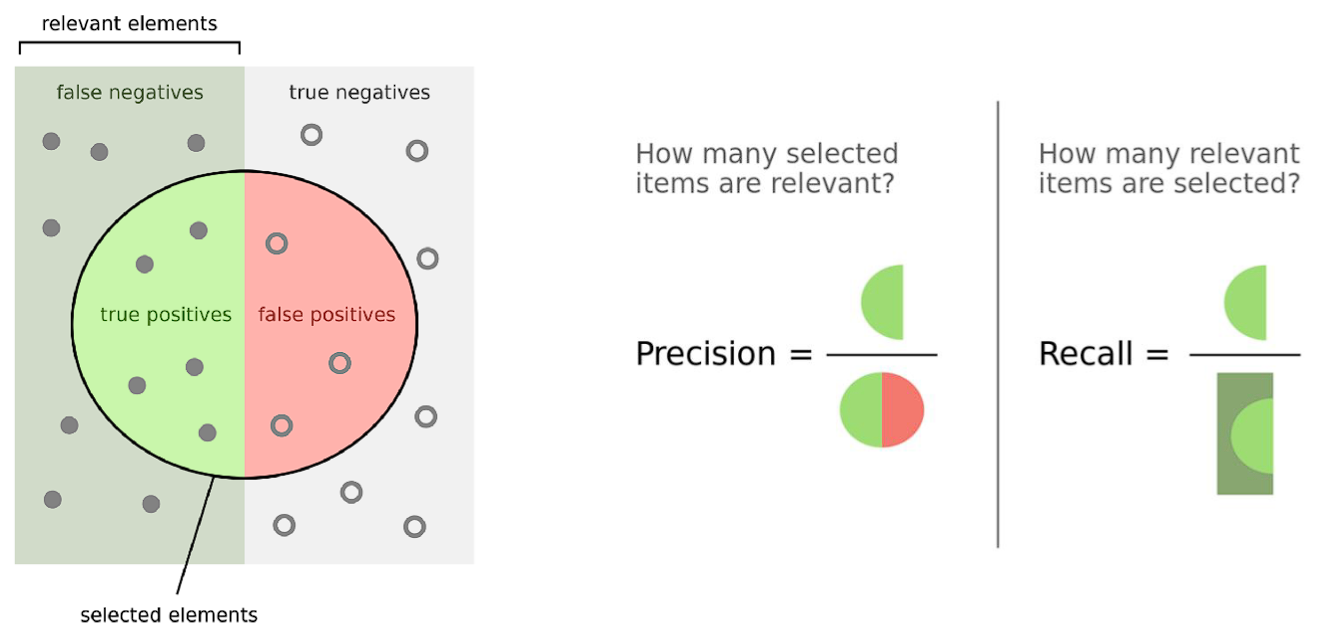
\includegraphics[width=1\textwidth]{assets/pics/recall-presisi.png}
            \captionsource{Ilustrasi \f{recall} dan presisi. Nilai \f{recall} dihitung sebagai rasio teks relevan yang diambil oleh sistem terhadap seluruh teks yang relevan dengan kueri $q$. Sedangkan nilai presisi dihitung sebagai rasio teks relevan yang diambil oleh sistem terhadap seluruh teks yang diambil oleh sistem.}{\citep{irlecture}.}
            \label{fig:recall-precision}
        \end{figure}
        Presisi dan \f{recall} adalah metrik yang paling sederhana untuk mengukur kemampuan dari suatu sistem pemeringkatan teks. \f{Recall} mengukur kemampuan sistem dalam mengembalikan semua teks yang relevan dengan kueri $q$ dari himpunan teks $\mathcal{D}$, sedangkan presisi mengukur kemampuan sistem dalam mengembalikan teks yang relevan dengan kueri $q$ dari himpunan teks $\mathcal{D}$. Untuk suatu kueri $q$, kumpulan teks $\mathcal{D} = \{d_1, d_2, ..., d_n\}$, dan barisan $k$ teks yang diambil oleh sistem, $D_k = (d_{i_1}, d_{i_2}, ..., d_{i_k})$, \f{recall} dan presisi dapat dihitung dengan \equ~\ref{eq:recall} hingga \equ~\ref{eq:presisi}.
        \begin{align}
            \label{eq:recall}
            \text{recall}(q, D_k)\text{@k} &= \frac{\sum_{d \in D_k} \text{rel}(q, d)}{\sum_{d \in \mathcal{D}} \text{rel}(q, d)} \in [0, 1], \\
            \label{eq:presisi}
            \text{precision}(q, D_k)\text{@k} &= \frac{\sum_{d \in D_k} \text{rel}(q, d)}{|D_k|} \in [0, 1], \\
            \label{eq:rel}
            \text{rel}(q, d) &= \begin{cases} 
            1 & \text{jika } r > 1 \\
            0 & \text{jika } r = 0
            \end{cases}.
        \end{align}

        Sebagai contoh, jika terdapat 10 teks yang relevan dengan kueri $q$, dan sistem mengembalikan $k=100$ teks, namun hanya terdapat 5 teks yang relevan pada $D_k$  maka \f{recall} dan presisi dari sistem tersebut adalah 0.5 ($\frac{5}{10}$) dan 0.05 ($\frac{5}{100}$) masing-masing. Baik \f{recall} maupun presisi memiliki rentang nilai dari 0 hingga 1, dengan nilai 1 menunjukkan performa sistem yang terbaik. Perhitungan \f{recall} biasanya dilakukan untuk $k$ yang cukup besar ($k = 100,1000 $), sedangkan perhitungan presisi dilakukan untuk $k$ yang kecil ($k = 1, 3, 5$) \citep{irlecture}.


        \subsubsection{\f{Reciprocal Rank}}

        \begin{figure}
            \centering
            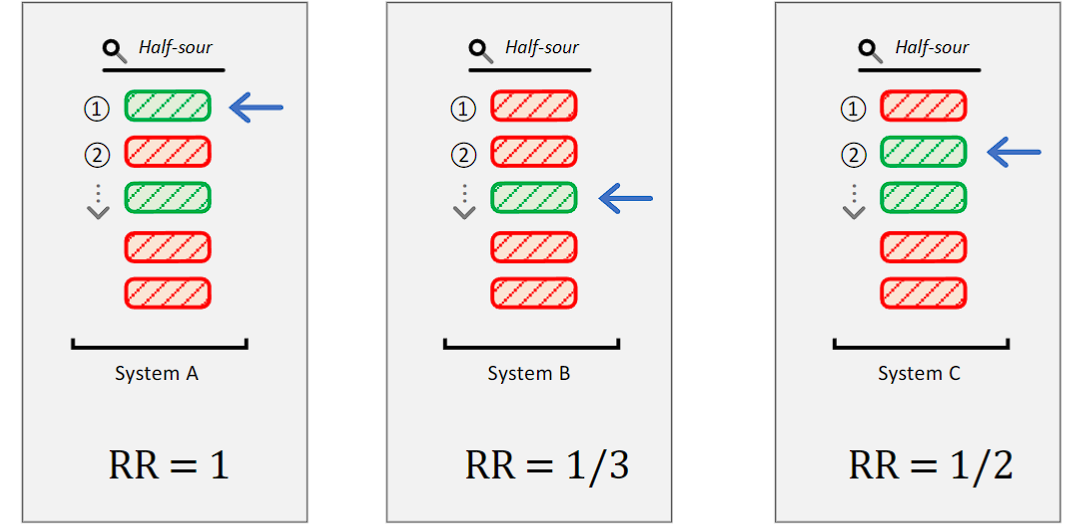
\includegraphics[width=1\textwidth]{assets/pics/rr.png}
            \captionsource{Ilustrasi \f{reciprocal rank} (RR). Kotak berwarnakan hijau menunjukkan teks yang relevan dengan kueri $q$ dan kotak berwarna merah menunjukkan teks yang tidak relevan dengan kueri $q$. Nilai RR pada sistem A, B, dan C berturut-turut adalah 1, 0.33, dan 0.5 karena posisi dari teks yang relevan pertama adalah 1, 3, dan 2.}{\citep{irlecture}.}
            \label{fig:reciprocal-rank}
        \end{figure}
        Metrik lainnya yang sering digunakan untuk mengukur performa sistem pemeringkatan adalah \f{reciprocal rank} (RR). Metrik RR menitikberatkan pada peringkat dari teks relevan pertama dengan kueri $q$. \equ~\ref{eq:reciprocal-rank-start} hingga \equ~\ref{eq:reciprocal-rank-end} menunjukkan cara menghitung RR dari suatu kueri $q$ dan barisan $k$ teks yang diambil oleh sistem.
        \begin{align}
            \text{RR}(q, D_k)\text{@k} &= \begin{cases}
                \label{eq:reciprocal-rank-start}
                \frac{1}{\text{FirstRank}(q, D_k)} & \text{jika } \exists d \in D_k \text{ dengan } \text{rel}(q, d) = 1 \\        
                0 & \text{jika } \forall d \in D_k, \text{ rel}(q, d) = 0 \\
                \end{cases} \in [0, 1], \\
                \label{eq:reciprocal-rank-end}
                \text{FirstRank}(q,D_k) &= \text{posisi teks relevan pertama } d\in D_k \text{ dengan } \text{rel}(q, d) = 1.
        \end{align}

        \pic~\ref{fig:reciprocal-rank} mengilustrasikan metrik RR. Pada gambar tersebut, nilai RR dari sistem A adalah 1 $(\frac{1}{1})$ karena posisi dari teks yang relevan pertama adalah 1. Nilai RR dari sistem B dan sistem C masing-masing adalah  0.33 $(\frac{1}{3})$ dan 0.5 $(\frac{1}{2})$ karena posisi dari teks yang relevan pertama adalah 3 dan 2. Selain itu, jika tidak terdapat teks yang relevan dengan kueri $q$ pada $D_k$, nilai RR dari sistem tersebut adalah 0. 

    \subsubsection{\f{Normalized Discounted Cumulative Gain} (nDCG)}

        \begin{figure}
            \centering
            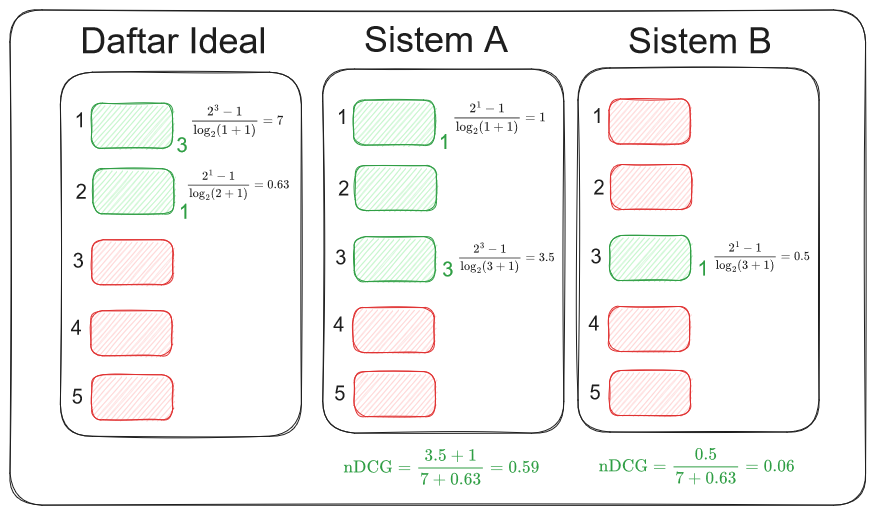
\includegraphics[width=1\textwidth]{assets/pics/contohnDCG.png}
            \captionsource{Ilustrasi perhitungan NDCG. Kotak berwarna hijau menunjukkan teks yang relevan dengan kueri $q$ dan kotak berwarna merah menunjukkan teks yang tidak relevan dengan kueri $q$ serta nilai disebelah kotak berwarnakan hijau menunjukkan \f{judgements} $r$. Nilai NDCG dari sistem A, B, adalah rasio antara DCG dari sistem tersebut dengan DCG dari sistem ideal.}{\citep{irlecture}, telah diolah kembali.}
            \label{fig:ndcg}
        \end{figure}
        \f{Normalized Discounted Cumulative Gain} (NDCG) adalah metrik yang umumnya digunakan untuk mengukur kualitas dari pencarian situs web. Tidak seperti metrik yang telah disebutkan sebelumnya, nDCG dirancang untuk suatu $r$ yang tak biner. \equ~\ref{eq:ndcg-start} hingga \equ~\ref{eq:ndcg-end} menunjukkan cara menghitung NDCG dari suatu kueri $q$ dan barisan $k$ teks yang diambil oleh sistem.
        \begin{align}
            \label{eq:ndcg-start}
            \text{nDCG}(q, D_k)\text{@k} &= \frac{\text{DCG}(q, D_k)\text{@k}}{\text{DCG}(q, D_k^{\text{ideal}})\text{@k}} \in [0, 1], \\
            \label{eq:dcg}
            \text{DCG}(q, D_k)\text{@k} &= \sum_{d \in D_k} \frac{2^{\text{rel}(q, d)} - 1}{\log_2(\text{rank}(d, D_k) + 1)}, \\
            \text{rank}(d,D_k) &= \text{Posisi } d \text{ dalam } D_k, \\
            \text{rel}(q, d) &= r.
            \label{eq:ndcg-end}
        \end{align}

        Perhitungan \f{discounted cumulative gain} (DCG) pada \equ~\ref{eq:dcg} dapat dijelaskan menjadi dua faktor berikut:
        \begin{enumerate}
            \item Faktor $2^{\text{rel}(q, d)} - 1$ menunjukkan bahwa teks yang lebih relevan akan memiliki nilai yang lebih tinggi dari teks yang kurang relevan untuk posisi teks yang sama.
            \item Faktor $\frac{1}{\log_2(\text{rank}(d, D_k) + 1)}$ menunjukkan bahwa teks yang relevan yang muncul pada peringkat tinggi akan memiliki nilai yang lebih besar dari teks dengan relevansi yang sama, tetapi muncul peringkat rendah.
        \end{enumerate}

        Nilai dari NDCG pada \equ~\ref{eq:ndcg-start} adalah nilai DCG pada barisan teks $D_k$ yang dinormalisasi oleh nilai DCG pada barisan teks ideal $D_k^{\text{ideal}}$. Barisan teks ideal $D_k^{\text{ideal}}$ adalah barisan teks yang diurutkan berdasarkan relevansinya dengan kueri $q$.


\section{Pemeringkatan Teks dengan Statistik}
        Untuk mengambil $k$ teks dari kumpulan $\mathcal{D}$ diperlukan suatu fungsi skor $\text{score}(q, d, \mathcal{D})$ yang mengukur relevansi antara kueri $q$ dan teks $d$. Dengan mencari skor antara $q$ terhadap semua teks pada $\mathcal{D}$, barisan teks $D_k = (d_{i_1}, d_{i_2},\dots, d_{i_k})$ dipilih sehingga $\text{score}(q, d_{i_1},\mathcal{D}) \geq \text{score}(q, d_{i_2}, \mathcal{D}) \geq \dots \geq \text{score}(q, d_{i_k},\mathcal{D})$ adalah $k$ teks dengan skor tertinggi.
        Bagian ini menjelaskan dua fungsi skor statistik sederhana yang menjadi \f{baseline} ketika membandingkan performa dari model pemeringkatan teks yang lebih kompleks. \sect~\ref{sec:tfidf} menjelaskan fungsi skor statistik yang berdasarkan pada frekuensi kemunculan kata dan tingkat \f{rarity} kata dalam kumpulan teks. Selanjutnya, \sect~\ref{sec:bm25} membahas fungsi skor statistik yang menjadi \f{baseline} dalam penelitian ini.
    \subsection{\f{Term Frequency - Inverse Document Frequency} (TF-IDF)}
    \label{sec:tfidf}
 
    Fungsi skor TF-IDF adalah fungsi skor statistik yang menghitung $\text{score}(q,d,\mathcal{D})$ antara kueri $q$ dan teks $d$ dengan menghitung frekuensi kemunculan kata dan tingkat \f{rarity} kata. Untuk suatu kueri $q$, misalkan $T_q= \{t_1, t_2, \dots, t_{L_1}\}$ adalah himpunan kata yang terdapat pada kueri $q$. Misalkan juga $T_d = \{t_1, t_2, \dots, t_n\}$ adalah himpunan kata yang terdapat pada teks $d$. Nilai skor antara $q$ dan $d$ diberikan oleh persamaan \equ~\ref{eq:tfidf-start} sampai \equ~\ref{eq:tfidf-end}.
    \begin{align}
        \label{eq:tfidf-start}
        \text{score}(q,d,\mathcal{D}) &= \sum_{t \in T_q \cap T_d} \text{TF-IDF}(t, d, \mathcal{D}) \\
        \label{eq:tf-idf-weight}
        \text{TF-IDF}(t, d, \mathcal{D}) &= \text{tf}(t, d) \times \text{idf}(t, \mathcal{D}) \\
        \text{tf}(t, d) &= \frac{\text{Count}(t, d)}{|d|} \\
        \text{Count}(t, d) &= \text{jumlah kemunculan } t \text{ dalam } d \\
        \text{idf}(t, \mathcal{D}) &= \begin{cases}
            \log_2\left(\frac{|\mathcal{D}|}{\text{df}(t, \mathcal{D})}\right) & \text{jika } \text{df}(t, \mathcal{D}) > 0 \\
            0 & \text{jika } \text{df}(t, \mathcal{D}) = 0
        \end{cases} \\
        \text{df}(t, \mathcal{D}) &= \text{jumlah teks pada } \mathcal{D} \text{ yang mengandung } t
        \label{eq:tfidf-end}
    \end{align}

    Skor untuk pasangan $(q,d)$ dihitung dengan menjumlahkan skor TF-IDF dari setiap kata yang terdapat pada kueri $q$ dan teks $d$. skor TF-IDF dari suatu kata $t$ adalah perkalian antara \f{term frequency} $\text{tf}(q,d)$ dan \f{inverse document frequency} $\text{idf}(t,\mathcal{D})$. Fungsi skor pada \equ~\ref{eq:tfidf-start} dapat dijelaskan menjadi dua faktor utama berikut:
    \begin{enumerate}
        \item Faktor $\text{tf}(t, d)$ menunjukkan bahwa nilai TF-IDF meningkat seiring dengan bertambahnya frekuensi kemunculan kata $t$ pada teks $d$.
        \item Faktor $\text{idf}(t, \mathcal{D})$ menunjukkan bahwa nilai TF-IDF meningkat seiring dengan \textit{rarity} dari kata $t$ pada himpunan teks $\mathcal{D}$. Akibatnya, kata yang jarang muncul pada himpunan teks $\mathcal{D}$ yang muncul pada suatu teks tertentu akan menghasilkan skor yang tinggi. Sementara itu, kata-kata yang sering muncul pada koleksi teks $\mathcal{D}$ memiliki nilai \textit{downgraded}. \pic~\ref{fig:idf-graph} menunjukkan grafik dari fungsi $\text{idf}$.
    \end{enumerate}
    \begin{figure}
    \centering
    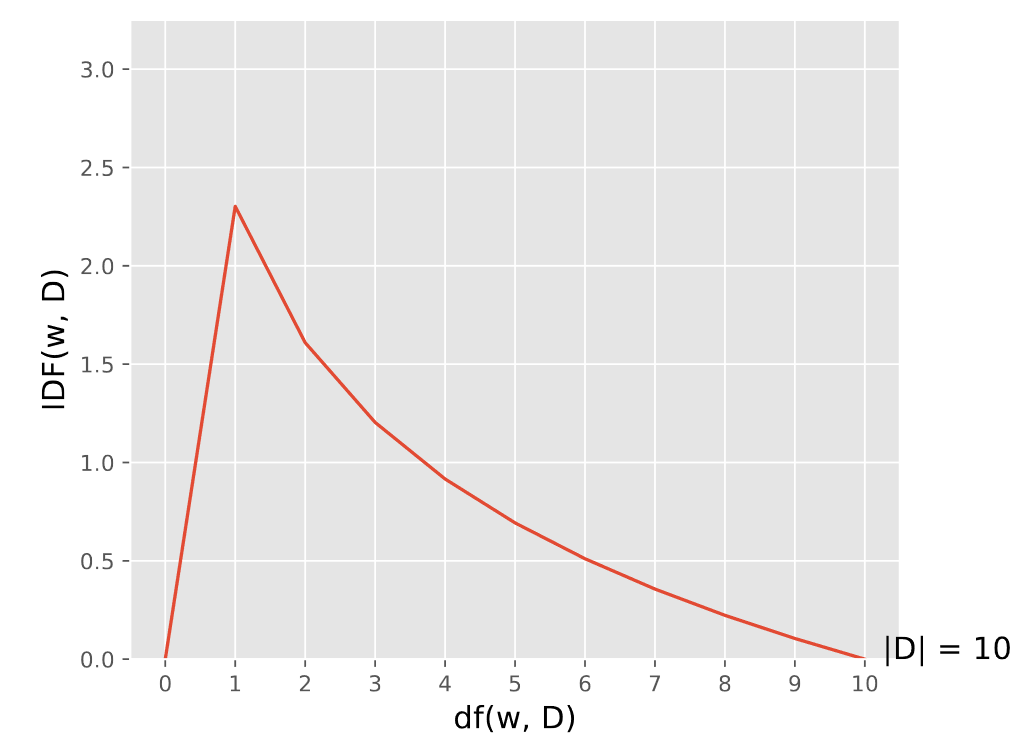
\includegraphics[width=0.75\textwidth]{assets/pics/idf-graph.png}
        \captionsource{Grafik dari fungsi $\text{idf}$. Nilai idf menurun seiring dengan bertambahnya nilai $\text{df}(t, \mathcal{D})$.}{\citep{stanfordir}.}
        \label{fig:idf-graph}
    \end{figure}

    Kata-kata seperti preposisi atau kata ganti akan menghasilkan skor TF-IDF yang sangat rendah. Hal ini menyiratkan bahwa kata-kata tersebut memiliki sedikit relevansi dalam teks dan bisa diabaikan. Di sisi lain, kata-kata yang muncul secara berlebihan dalam satu teks tetapi jarang muncul dalam teks lainnya akan menghasilkan nilai $\text{tf}(t, d)$ dan $\log \left(\frac{\mathcal{D}}{\text{df}(t, \mathcal{D})}\right)$ yang relatif besar. Dampaknya adalah skor TF-IDF yang dihasilkan juga menjadi signifikan. \pic~\ref{fig:tf-idf-matriks} menunjukkan contoh perhitungan skor TF-IDF untuk suatu kumpulan teks.

    
    \begin{figure}
        \centering
        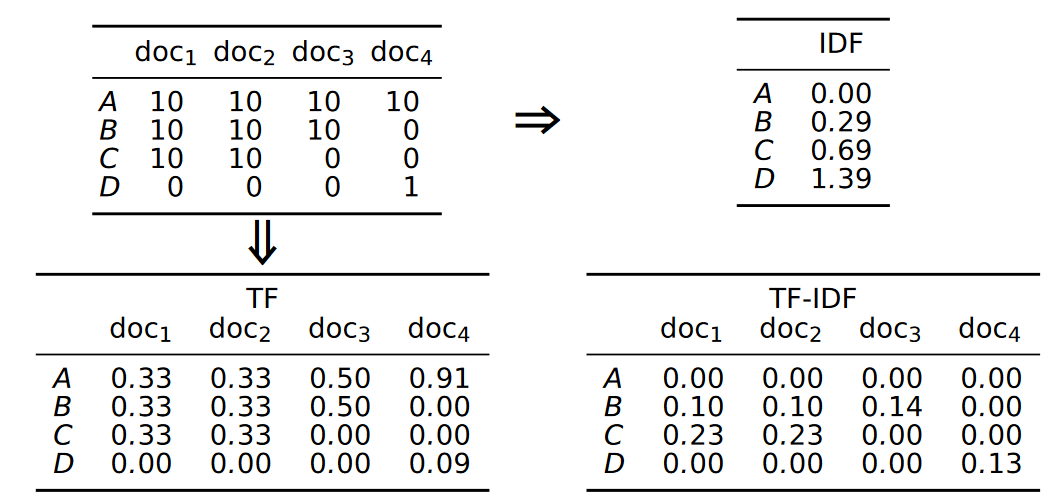
\includegraphics[width=1\textwidth]{assets/pics/tf-idf-matriks.png}
        \captionsource{Ilustrasi perhitungan skor TF-IDF untuk suatu kumpulan teks.}{\citep{stanfordir}.}
        \label{fig:tf-idf-matriks}
    \end{figure}
    \subsection{\f{Best Match 25} (BM25)}
    \label{sec:bm25}
    
    BM25 (\f{Best Match attempt} 25)  merupakan pengembangan dari fungsi skor TF-IDF dengan perbedaan utama pada fungsi nilai yang berkaitan dengan frekuensi kata -- digunakan $\text{score}_{\text{BM25}}(q,d)$ (\equ~\ref{eq:bm25-weight}) daripada $\text{tf}(q,d)$ (\equ~\ref{eq:tf-idf-weight}). Pada fungsi $\text{score}_{\text{BM25}(q,d)}$ terdapat 2 parameter yang dapat diatur, yaitu $b$, dan $k_1$. Setiap parameter mempunyai efek yang berbeda terhadap nilai $\text{score}_{\text{BM25}(q,d)}$ yang dihasilkan. Sebelum menjelaskan efek dari setiap parameter, \equ~\ref{eq:bm25scoring} hingga \equ~\ref{eq:bm25-end} menunjukkan cara menghitung skor relevansi dari suatu kueri $q$ dan teks $d$. 
    \begin{align}
        \label{eq:bm25scoring}
        \text{score}(q,d,\mathcal{D}) &= \sum_{t \in T_q \cap T_d} \text{BM25}(t, d, \mathcal{D}),\\
        \label{eq:bm25-weight}
        \text{BM25}(t, d, \mathcal{D}) &= \text{idf}_{\text{BM25}}(t, \mathcal{D}) \times \text{score}_{\text{BM25}}(q,d,\mathcal{D}), \\
        \text{score}_{\text{BM25}}(t,d) &= \frac{\text{tf}(t, d) \times (k_1 + 1)}{\text{tf}(t, d) + k_1 \times (1 - b + b \times \frac{|d|}{\text{avgdl}})}, \\
        \label{eq:smoothed-idf}
        \text{idf}_{\text{BM25}}(t, \mathcal{D}) &= \log\left(1+\frac{|\mathcal{D}| - \text{df}(t, \mathcal{D}) + 0.5}{\text{df}(t, \mathcal{D}) + 0.5}\right), \\
        \text{avgdl} &= \text{rata-rata panjang teks pada koleksi } \mathcal{D}.
        \label{eq:bm25-end}
    \end{align}
    Efek dari masing-masing parameter dan faktor pada $\text{score}_{\text{BM25}}(t,d)$ dapat dijelaskan sebagai berikut:
    \begin{enumerate}
        \item Faktor $\frac{|\text{d}|}{\text{avgdl}}$ pada $\frac{\text{tf}(t, d) \times (k_1 + 1)}{\text{tf}(t, d) + k_1 \times \left(1 - b + b \times \textcolor{black}{\frac{|d|}{\text{avgdl}}}\right)}$ men-\f{penalize} skor pada teks yang panjangnya lebih besar dari rata-rata panjang teks pada himpunan teks $\mathcal{D}$. \pic~\ref{fig:effect-bm25-long-doc} menjukkan efek dari perbedaan nilai $\text{avgdl}$ terhadap skor yang dihasilkan, makin besar rasio $\frac{|d|}{\text{avgdl}}$ makin kecil skor yang dihasilkan.
        \item Nilai $b$ menentukan seberapa besar efek dari faktor $\frac{|d|}{\text{avgdl}}$ terhadap skor yang dihasilkan. \pic~\ref{fig:effect-bm25-param-b} menunjukkan efek dari perbedaan nilai $b$ terhadap skor yang dihasilkan. Untuk $\frac{|d|}{\text{avgdl}}=1$, faktor $b$ tidak memiliki pengaruh terhadap skor. Nilai $b$ yang umum dipilih berada pada rentang $[0.5, 0.8]$ \citep{irlecture}.
        \item  Nilai $k_1$ men-\f{penalize} kemunculan kata $t$ pada teks $d$ yang berlebih. \pic~\ref{fig:effect-bm25-param-k} menunjukkan efek dari perbedaan nilai $k_1$ terhadap skor yang dihasilkan. untuk nilai $k_1$ yang ekstrim, nilai $\text{score}_{\text{BM25}}(t,d)$ hanya menjadi indikator saja dari kemunculan kata $t$ pada teks $d$. Nilai $k_1$ yang umum dipilih berada pada rentang $[1.2, 2.0]$ \citep{irlecture}.
    \end{enumerate}
    \begin{figure}
        \centering
        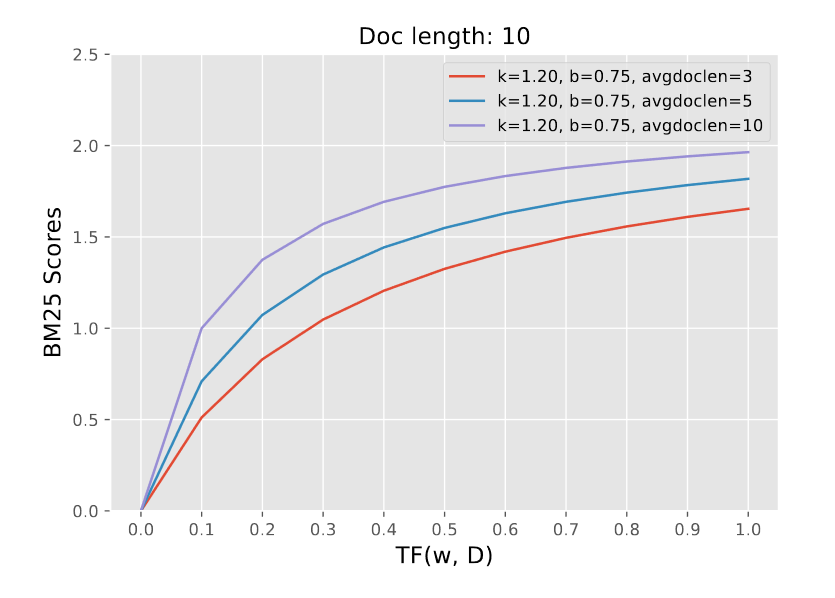
\includegraphics[width=0.75\textwidth]{assets/pics/effect-bm25-long-doc.png}
        \captionsource{Kumpulan grafik dari fungsi $\text{score}_{\text{BM25}}(t,d)$ dengan perbedaan nilai $\text{avgdl}$.}{\citep{stanfordir}.}
        \label{fig:effect-bm25-long-doc}
    \end{figure}

    \begin{figure}
        \centering
        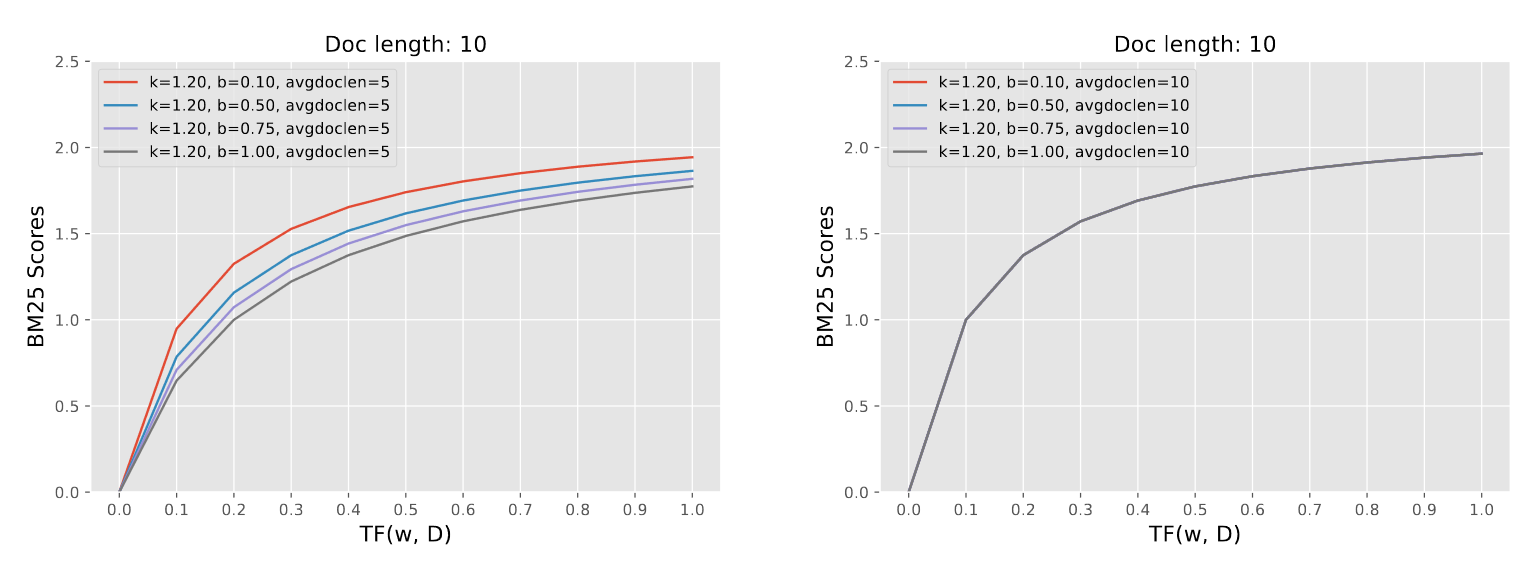
\includegraphics[width=1\textwidth]{assets/pics/effect-bm25-param-b.png}
        \captionsource{Kumpulan grafik dari fungsi $\text{score}_{\text{BM25}}(t,d)$ dengan perbedaan nilai $b$.}{\citep{stanfordir}.}
        \label{fig:effect-bm25-param-b}
    \end{figure}
    \begin{figure}
        \centering
        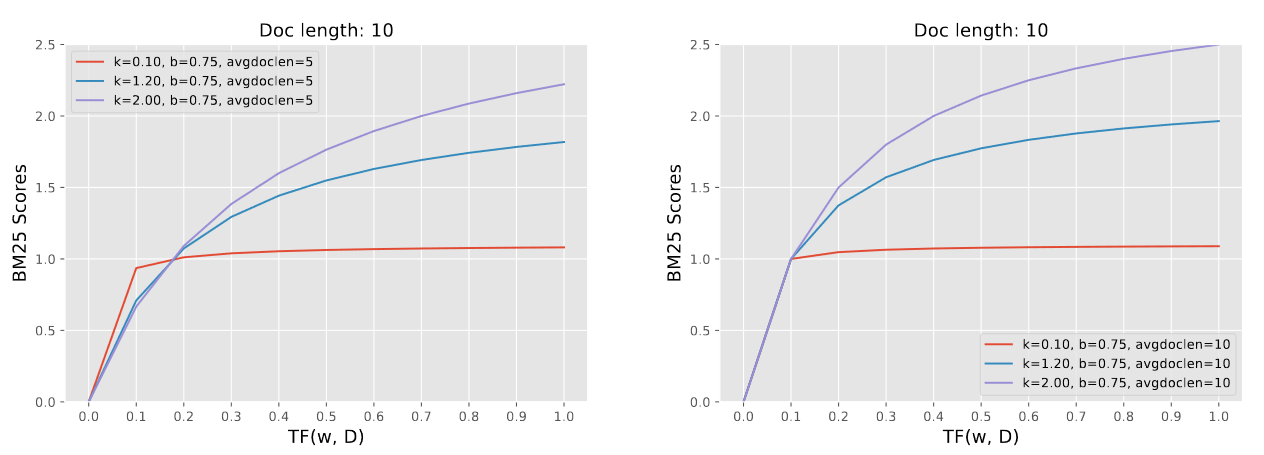
\includegraphics[width=1\textwidth]{assets/pics/effect-bm25-param-k.png}
        \captionsource{Kumpulan grafik dari fungsi $\text{score}_{\text{BM25}}(t,d)$ dengan perbedaan nilai $k_1$.}{\citep{stanfordir}.}
        \label{fig:effect-bm25-param-k}
    \end{figure}
    
    Perbedaan \f{minor} lainnya ada pada fungsi $\text{idf}$. Fungsi $\text{idf}$ pada BM25 merupakan versi \f{smoothing} dari $\text{idf}$ dengan tujuan untuk menghindari nilai $\text{idf}$ yang bernilai 0 ketika kata $t$ tidak muncul pada himpunan teks $\mathcal{D}$ -- semata-mata untuk konsistensi dengan asumsi bahwa kata $t$ yang tidak muncul pada himpunan teks $\mathcal{D}$ memiliki nilai $\text{idf}$ (\f{rarity}) yang paling tinggi. \pic~\ref{fig:smoothed-idf} menunjukkan perbedaan antara $\text{idf}_{BM25}$ dan $\text{idf}$. Perbedaan utamanya terjadi ketika $\text{df}(t,\mathcal{D}) = 0$, nilai dari  $\text{idf}_{BM25}$ tak nol dan mengikuti pola yang diharapkan. Ketika $\text{df}(t,\mathcal{D})>0$, nilai dari $\text{idf}_{\text{BM25}}$ dan $\text{idf}$ hampir serupa.

    \begin{figure}
        \centering
        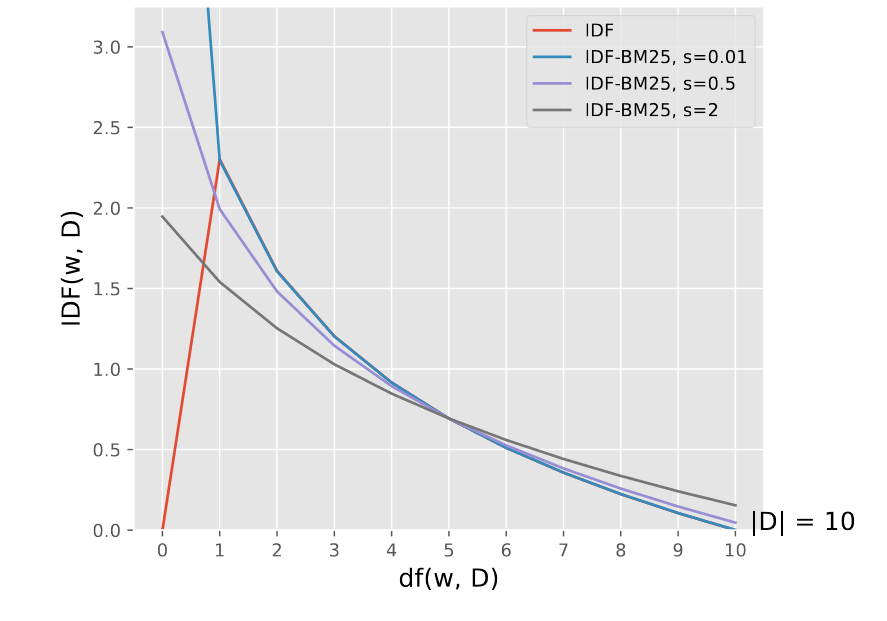
\includegraphics[width=0.75\textwidth]{assets/pics/smoothed-idf.png}
        \captionsource{Perbedaan antara $\text{idf}_{\text{BM25}}$ dan $\text{idf}$.}{\citep{stanfordir}.}
        \label{fig:smoothed-idf}
    \end{figure}


\section{\f{Deep Learning}}
    \begin{figure}
        \centering
        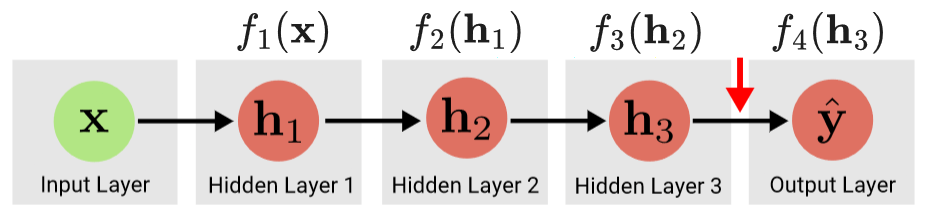
\includegraphics[width=0.50\textwidth]{assets/pics/dag-dl.png}
        \captionsource{Ilustrasi dari \f{Directed Acyclic Graph} (DAG) pada arsitektur \f{deep learning feed-forward neural network} (FFN).}{\citep{geiger2022deeplearning}, telah diolah kembali.}
        \label{fig:deep-learning-FFN-dag}
    \end{figure}
    Arsitektur \f{deep learning} merujuk pada model \f{machine learning} yang tersusun dari fungsi-fungsi terturunkan (yang biasa disebut sebagai \f{layer}), dimana komposisi antara fungsi-fungsi tersebut dapat digambarkan sebagai \f{directed acyclic graph} (DAG) yang memetakan suatu \f{input} ke suatu \f{output}. Biasanya, setiap fungsi dalam Arsitektur \f{deep learning} memiliki parameter yang ingin diestimasi atau dicari dengan data.
    
    \pic~\ref{fig:deep-learning-FFN-dag} menunjukkan arsitektur \f{deep learning} yang sederhana, yaitu \f{feed-forward neural network} (FFN). Pada \pic~\ref{fig:deep-learning-FFN-dag}, \f{input} $\mathbf{x}$ akan dipetakan ke \f{output} $\mathbf{\hat y}$ melalui serangkaian fungsi $f_1, f_2, f_3,f_4$ yang disebut sebagai \f{layer}. Setiap \f{layer} $f_i$ memiliki parameter $\theta_i$ yang akan diestimasi dengan data. Selain itu, \f{output} dari \f{layer} $f_i$ akan menjadi \f{input} dari \f{layer} $f_{i+1}$. \f{Output} dari \f{layer} $f_4$ adalah \f{output} dari model. Model pada \pic~\ref{fig:deep-learning-FFN-dag} dapat ditulis sebagai \equ~\ref{eq:deep-learning-FFN-dag}.
    \begin{align}
        \label{eq:deep-learning-FFN-dag}
        \mathbf{\hat y} = f_{\text{model}}(\mathbf{x}; \bm{\theta}) &= f_4(f_3(f_2(f_1(\mathbf{x}; \bm{\theta}_1); \bm{\theta}_2); \bm{\theta}_3); \bm{\theta}_4),
    \end{align}
    dengan $\bm{\theta} = \{\bm{\theta}_1, \bm{\theta}_2, \bm{\theta}_3, \bm{\theta}_4\}$ adalah parameter dari model.

    \subsection{\f{Multilayer Perceptron} (MLP)}

    \f{Multi-layer perceptron} (MLP) adalah \f{feed-forward neural network} dengan setiap fungsi $f_i$ adalah fungsi linear yang diikuti oleh fungsi aktivasi non-linear $\phi$  yang diterapkan \f{element-wise} pada setiap \f{output}-nya. \f{Hyperparameter} (parameter yang dipilih prior proses pelatihan dilakukan) lainnya selain fungsi aktivasi adalah kedalamaan model $L$, dan dimensi \f{output} dari setiap \f{layer} $d_1, d_2, \dots, d_L$.

    Untuk permasalahan regresi dengan \f{input} $\mathbf{x}\in \mathbb{R}^{d_0}$ dan \f{output} $\mathbf{y} \in \mathbb{R}^{d_L}$, \equ~\ref{eq:FFN-regesi-start} hingga \equ~\ref{eq:FFN-regesi-end} menunjukkan arsitektur MLP untuk permasalahan regresi dengan $L$ \f{layer} dan fungsi aktivasi $\phi$.
    \begin{align}
        \label{eq:FFN-regesi-start}
        f_{\text{model}}(\mathbf{x};\bm{\theta}) &= f_L(f_{L-1}(\dots f_1(\mathbf{x})) \dots), \\
        f_L(\mathbf{x}) &= \mathbf{x} \mathbf{W}_L + \mathbf{b}_L \in \mathbb{R}^{d_L}, \\
        f_l(\mathbf{x};\mathbf{W}_l, \mathbf{b_l}) &= \phi( \mathbf{x} \mathbf{W}_l + \mathbf{b}_l) \in \mathbb{R}^{d_l}, \quad l = 1, 2, \dots, L-1,
        \label{eq:FFN-regesi-end}
    \end{align} 
    dengan keterangan sebagai berikut:
    \begin{flalign*}
        \phi(\mathbf{x}) &= \text{fungsi aktivitasi non-linear},&& \\
        \bm{\theta} &= \{\mathbf{W}_1, \mathbf{b}_1, \mathbf{W}_2, \mathbf{b}_2, \dots, \mathbf{W}_L, \mathbf{b}_L\},&& \\
        \mathbf{W}_l &= \text{matriks bobot}  \in \mathbb{R}^{d_{l-1} \times d_l},&& \\
        \mathbf{b}_l &= \text{vektor bias} \in \mathbb{R}^{d_l}.&&
    \end{flalign*}

    Untuk Permasalahan Klasifikasi Biner dengan \f{input} $\mathbf{x}\in \mathbb{R}^{d_0}$ dan \f{output} $y \in \{0, 1\}$, \equ~\ref{eq:FFN-klasifikasi-biner-start} hingga \equ~\ref{eq:FFN-klasifikasi-biner-end} menunjukkan arsitektur MLP untuk permasalahan klasifikasi biner.
    \begin{align}
        \label{eq:FFN-klasifikasi-biner-start}
        f_{\text{model}}(\mathbf{x};\bm{\theta}) &= f_L(f_{L-1}(\dots f_1(\mathbf{x})) \dots), \\
        f_L(\mathbf{x}) &= \sigma(\mathbf{x} \mathbf{W}_L + \mathbf{b}_L), \\
        \sigma(x) &= \frac{1}{1 + e^{x}} \in (0, 1), \\
        \text{decision}(\mathbf{x};\bm{\theta}) &= \begin{cases}
        1 & \text{jika } f_{\text{model}}(\mathbf{x};\bm{\theta}) \geq \text{threshold} \\
        0 & \text{jika } f_{\text{model}}(\mathbf{x};\bm{\theta}) < \text{threshold},
        \end{cases} \\
        \label{eq:FFN-klasifikasi-biner-end}
        \text{threshold}&\in [0, 1].
    \end{align}

    Perbedaan utama antara MLP untuk permasalahan regresi dan klasifikasi adalah fungsi aktivasi pada \f{output layer}. Pada permasalahan regresi, fungsi aktivasi pada \f{output layer} adalah fungsi identitas, sedangkan pada permasalahan klasifikasi, fungsi aktivasi pada \f{output layer} adalah fungsi \f{sigmoid}. Tujuan pengunaan fungsi \f{sigmoid} pada permasalahan klasifikasi adalah untuk memastikan bahwa \f{output} dari model berada pada rentang $[0, 1]$, nilai tersebut dapat diinterpretasikan sebagai probabilitas $\mathbf{x}$ termasuk pada kelas positif. Selain itu, \f{threshold} pada \equ~\ref{eq:FFN-klasifikasi-biner-end} digunakan untuk menentukan kelas dari $\mathbf{x}$.

    \subsection{Fungsi Aktivasi}

    Fungsi aktivasi pada setiap fungsi $f_i$ pada \f{multilayer perceptron} digunakan untuk menambahkan non-linearitas pada model. Sebab, tanpa adanya fungsi aktivasi non-linear, model \f{multilayer perceptron} akan menjadi model linear. Selain itu, fungsi aktivasi juga biasanya adalah fungsi yang terturunkan, meskipun tidak perlu terturunkan disetiap titik. \tab~\ref{tab:activation-function} menunjukkan beberapa fungsi aktivasi yang sering digunakan pada \f{multilayer perceptron}. \pic~\ref{fig:activation-function} menunjukkan grafik dari fungsi aktivasi pada \tab~\ref{tab:activation-function} dan turunannya.
    \begin{table}
        \centering
        \caption{Beberapa fungsi aktivasi yang sering digunakan pada \f{multilayer perceptron}.}
        \label{tab:activation-function}
        \begin{tabular}{|c|c|}
            \hline
            \textbf{Fungsi Aktivasi} & \textbf{Persamaan} \\
            \hline
            \hline
            Sigmoid & $\sigma(x) = \frac{1}{1 + e^{-x}}$ \\
            \hline
            Tanh & $\tanh(x) = \frac{e^x - e^{-x}}{e^x + e^{-x}}$ \\
            \hline
            ReLU & $\text{ReLU}(x) = \max(0, x)$ \\
            \hline
            Leaky ReLU & $\text{LeakyReLU}(x) = \max(\alpha x, x), \alpha \in [0, 1]$ \\
            \hline
        \end{tabular}
    \end{table}
    \begin{figure}
        \centering
        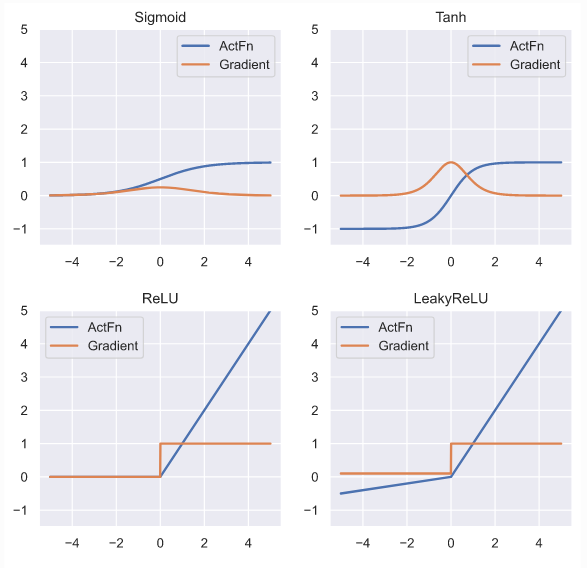
\includegraphics[width=0.5\textwidth]{assets/pics/act_function.png}
        \captionsource{Grafik dari fungsi aktivasi pada \tab~\ref{tab:activation-function} dan turunannya.}{\citep{uvadlc}.}
        \label{fig:activation-function}
    \end{figure}


    \subsection{Fungsi \f{Loss}}
    Misalkan $\mathcal{D} = \{(\mathbf{x}_1, y_1), (\mathbf{x}_2, y_2), \dots, (\mathbf{x}_n, y_n)\}$ adalah \f{dataset} yang terdiri dari $n$ pasangan \f{input} dan \f{output}. Parameter $\bm{\theta}$ pada $f_{\text{model}}$ diestimasi dengan melakukan \f{fitting} pada \f{dataset} $\mathcal{D}$. Untuk melakukan \f{fitting} pada \f{dataset} $\mathcal{D}$, diperlukan suatu fungsi \f{loss} yang mengukur seberapa baik hasil pemetaan $f_{\text{model}}$ pada \f{input} $\mathbf{x}_i$ terhadap \f{output} $\mathbf{y}_i$. Meskipun sembarang fungsi yang terturunkan dapat digunakan sebagai fungsi \f{loss}, namun pemilihan fungsi \f{loss} berdasarkan \f{maximum likelihood estimation} (MLE) lebih disarankan. 
    
    Untuk permasalahan klasifikasi biner, fungsi \f{loss} yang sering digunakan adalah \f{binary cross entropy} (BCE) seperti yang ditinjukkan pada \equ~\ref{eq:bce}. Penurunan fungsi \f{loss} BCE dengan mengikuti prinsip MLE yang akan dijelaskan pada bagian berikut.
    
    Misalkan $y_i \mid \mathbf{x}$ mengikuti distribusi bernoulli dengan parameter $\text{p} = f_{\text{model}}(\mathbf{x};\bm{\theta})$ yang saling independen antara satu sama lainnya. \equ~\ref{eq:definisi-random-variable} menunjukkan definisi dari $y_i \mid \mathbf{x}$.
    \begin{align}
        \label{eq:definisi-random-variable}
        y_i \mid \mathbf{x} &\overset{\text{iid}}{\sim} \text{Bernoulli}(f_{\text{model}}(\mathbf{x};\bm{\theta})), \\
        p(y_i \mid \mathbf{x}) &= f_{\text{model}}(\mathbf{x};\bm{\theta})^{y_i} (1 - f_{\text{model}}(\mathbf{x};\bm{\theta}))^{1 - y_i}.
    \end{align} 

    Fungsi $\f{likelihood}$ dari $\bm{\theta}$ terhadap \f{dataset} $\mathcal{D}$ dapat ditulis sebagai berikut:
    \begin{align}
        \mathcal{L}(\bm{\theta}) &= \prod_{i=1}^N p(y_i \mid \mathbf{x}_i; \bm{\theta}).
    \end{align}

    Dengan prinsip MLE, parameter $\bm{\theta}$ yang dicari adalah parameter $\bm{\theta}$ yang memaksimalkan fungsi \f{likelihood} $\mathcal{L}(\bm{\theta})$,
    \begin{align}
        \bm{\theta}_{\text{MLE}} &= \arg\max_{\bm{\theta}} \mathcal{L}(\bm{\theta}).
    \end{align}

    Untuk mempermudah perhitungan, fungsi \f{likelihood} diubah menjadi negatif \f{log-likelihood} $\mathcal{\ell}(\bm{\theta})$, sehingga permasalahan optimasi dapat ditulis seperti \equ~\ref{eq:log-likelihood} hingga \equ~\ref{eq:log-likelihood-end}.
    \begin{align}
        \label{eq:log-likelihood}
        \ell{(\bm{\theta})} &= -\log\mathcal{L}(\bm{\theta}), \\
        &= -\sum_{i=1}^N \log\left(p(y_i \mid \mathbf{x}_i; \bm{\theta})\right), \\
        \label{eq:log-likelihood-end}
        \bm{\theta}_{\text{MLE}} &= \arg\min_{\bm{\theta}} \ell(\bm{\theta}).
    \end{align} 

    Dengan mengganti $p(y_i \mid \mathbf{x}_i; \bm{\theta})$ dengan fungsi distribusi-nya, maka fungsi \f{loss} yang digunakan untuk permasalahan klasifikasi biner adalah \f{binary cross entropy} (BCE) seperti pada \equ~\ref{eq:bce}. \pic~\ref{fig:dl-training-graph-dag} mengilustrasikan \f{directed acyclic graph} (DAG) dari model ketika proses pelatihan dilakukan.
    \begin{align}
        \bm{\theta}_{\text{MLE}} &= \arg\min_{\bm{\theta}}\sum_{i=1}^{N}\underbrace{-y_i \log\left(f_{\text{model}}(\mathbf{x}_i; \bm{\theta})\right) - (1 - y_i) \log\left(1 - f_{\text{model}}(\mathbf{x}_i; \bm{\theta})\right)}_{\text{Binary Cross Entropy Loss } L(y_i, f_{\text{model}}(\mathbf{x}_i; \bm{\theta}))}, \\
        \label{eq:bce} 
        L(y_i, f_{\text{model}}(\mathbf{x}_i; \bm{\theta})) &= -y_i \log\left(f_{\text{model}}(\mathbf{x}_i; \bm{\theta})\right) - (1 - y_i) \log\left(1 - f_{\text{model}}(\mathbf{x}_i; \bm{\theta})\right).
    \end{align}
    \begin{figure}
        \centering
        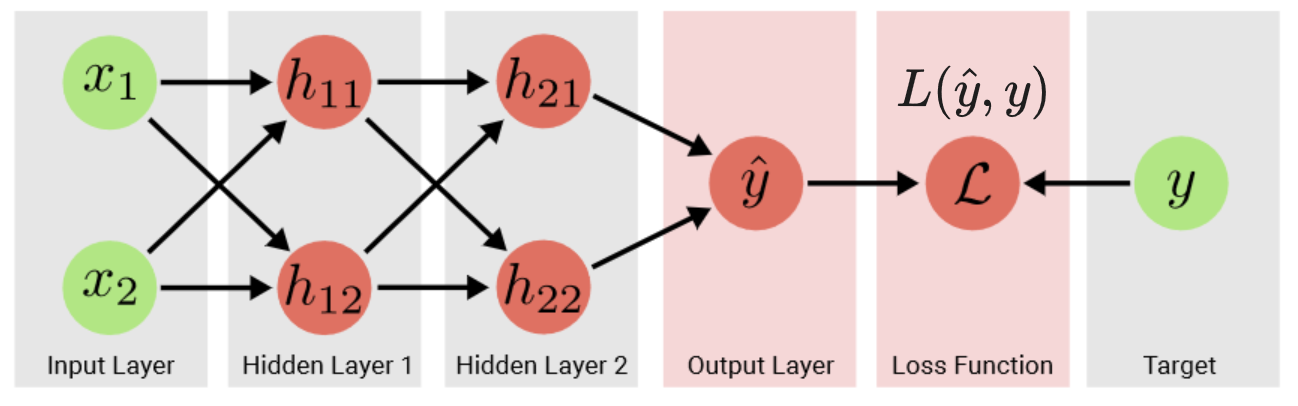
\includegraphics[width=1\textwidth]{assets/pics/dl-training-graph.png}
        \captionsource{Ilustrasi dari \f{Directed Acyclic Graph} (DAG) pada model \f{deep learning} ketika proses pelatihan dilakukan.}{\citep{geiger2022deeplearning}, telah diolah kembali.}
        \label{fig:dl-training-graph-dag}
    \end{figure}

    Untuk mendapatkan $f_\text{model}$ dengan performa yang baik, dibutuhkan model dengan nilai $\ell(\bm{\theta})$ seminimum mungkin. Namun, pencarian $\bm{\theta}$ sehingga $ \ell (\bm{\theta})$ minumum secara analitik tidak dapat dilakukan karena non-linearitas yang ada pada model, dengan kata lain solusi dari $\nabla_{\bm{\theta}} \ell(\bm{\theta}) = 0$ tidak dapat dicari secara analitik. Sebagai gantinya, pencarian $\bm{\theta}$ dilakukan secara numerik dengan menggunakan metode \f{gradient descent} yang akan dijelaskan pada bagian selanjutnya.
    
\subsection{\f{Optimasi} Parameter}

    \f{Gradient descent} adalah metode numerik yang digunakan untuk mencari nilai $\bm{\theta}$ yang meminimalkan fungsi \f{loss} $\ell(\bm{\theta})$. Pada metode \f{gradient descent}, nilai $\bm{\theta}$ di-\f{update} secara iteratif dengan mengikuti arah negatif dari \f{gradient} $\nabla_{\bm{\theta}} \ell(\bm{\theta})$ yang menunjukkan arah dari penurunan fungsi \f{loss} $\ell(\bm{\theta})$. Untuk kumpulan data $\mathcal{D} = \{(\mathbf{x}_1, y_1), (\mathbf{x}_2, y_2), \dots, (\mathbf{x}_n, y_n)\}$, \equ~\ref{eq:gradient-descent} menunjukkan algoritma \f{gradient descent} untuk mencari nilai $\bm{\theta}$.
    \begin{align}
        \label{eq:gradient-descent}
        \bm{\theta}^{(t+1)} &= \bm{\theta}^{(t)} - \eta \frac{1}{n} \sum_{i=1}^{n} \nabla_{\bm{\theta}} L(y_i, f_{\text{model}}(\mathbf{x}_i; \bm{\theta}^{(t)})),
    \end{align}
    dengan $\eta \in \mathbb{R}^+$ adalah \f{learning rate} yang menentukan seberapa besar perubahan pada $\bm{\theta}$ pada setiap iterasi.

    Perlu diketahui bahwa pada metode \f{gradient descent} memperbarui parameter dengan mengambil rata-rata \f{gradient} dari semua data pada \f{dataset} pelatihan $\mathcal{D}$. Hal ini menciptakan masalah ketika model menggunakan banyak parameter dan jumlah data pada \f{datasets} latih besar, yaitu komputasi \f{forward pass} dan \f{backward pass} menjadi sangat mahal dan diperlukan memori yang besar untuk menyimpan gradien dari semua data pada \f{dataset} latih. Untuk mengatasi masalah tersebut, digunakan metode \f{stochastic gradient descent} (SGD) dimana setiap \f{update} dari parameter $\bm{\theta}$ dihitung dengan mengambil rata-rata \f{gradient} dari sebagian data pada \f{dataset} $\mathcal{B}\subseteq\mathcal{D}$. \equ~\ref{eq:stochastic-gradient-descent} menunjukkan algoritma \f{stochastic gradient descent}.
    \begin{align}
        \mathcal{B} = \{(\mathbf{x}_{i_1}, y_{i_1}), (\mathbf{x}_{i_2}, y_{i_2}), \dots, (\mathbf{x}_{i_b}, y_{i_b})\} &\subseteq \mathcal{D}, \mid \mathcal{B} \mid \ll \mid \mathcal{D} \mid, \\
        \label{eq:stochastic-gradient-descent-approx}
        \nabla_{\bm{\theta}}{L_\mathcal{B}}(\bm{\theta}) &= 
         \frac{1}{b} \sum_{i=1}^{b} \nabla_{\bm{\theta}} L(y_{i}, f_{\text{model}}(\mathbf{x}_{i}; \bm{\theta})), \\
        \label{eq:stochastic-gradient-descent}
        \bm{\theta}^{(t+1)} &= \bm{\theta}^{(t)} - \eta \nabla_{\bm{\theta}} \mathcal{L_B}(\bm{\theta}^{(t)}).
    \end{align}

    \f{Hyperparameter} \f{learning rate} mengatur laju dari perubahan parameter $\bm{\theta}$ pada setiap iterasi pembaruan. Dengan demikian, pemilihan \f{learning rate} berpengaruh terhadap kekonvergenan optimasi yang dilakukan. Jika \f{learning rate} yang digunakan terlalu kecil, model membutuhkan waktu yang jauh lebih lama untuk mencapai nilai parameter $\bm{\theta}$ yang optimal. Di lain sisi, pemilihan \f{learning rate} yang terlalu besar dapat membuat model tidak dapat menemukan nilai parameter $\bm{\theta}$ yang optimal. \pic~\ref{fig:learning-rate-bad} mengilustrasikan proses pembaruan parameter $\bm{\theta}$ dengan \f{learning rate} yang terlalu kecil dan terlalu besar, dan \pic~\ref{fig:learning-rate-good} mengilustrasikan proses pembaruan parameter $\bm{\theta}$ dengan \f{learning rate} yang baik.
\begin{figure}
    \centering
    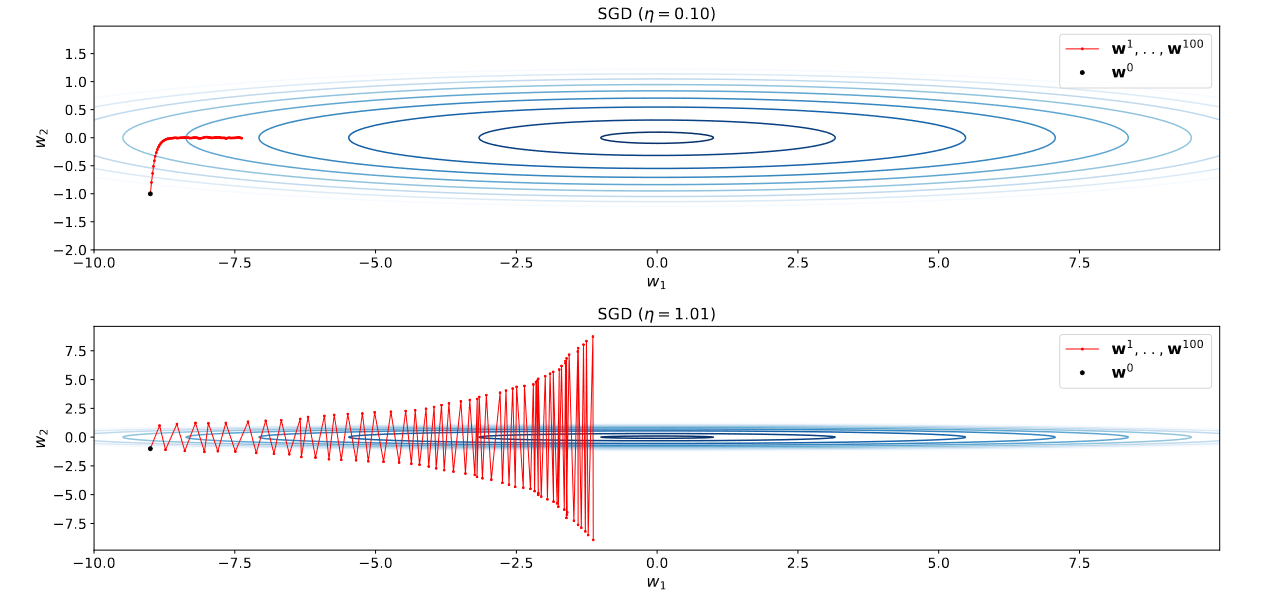
\includegraphics[width=1\textwidth]{assets/pics/learning-rate-bad.png}
    \captionsource{Seratus iterasi pertama dari pembaruan parameter $\bm{\theta} = \{w_1, w_2\}$ dengan \f{learning rate} yang terlalu kecil dan terlalu besar.}{\citep{geiger2022deeplearning}.}
    \label{fig:learning-rate-bad}
\end{figure}

\begin{figure}
    \centering
    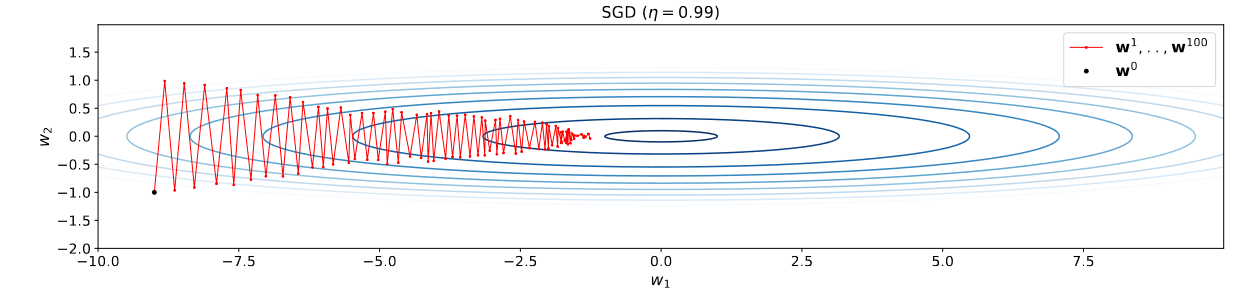
\includegraphics[width=1\textwidth]{assets/pics/learning-rate-good.png}
    \captionsource{Seratus iterasi pertama dari pembaruan parameter $\bm{\theta} = \{w_1, w_2\}$ dengan \f{learning rate} yang baik.}{\citep{geiger2022deeplearning}.}
    \label{fig:learning-rate-good}
\end{figure}

Untuk mempercepat proses pembaruan parameter $\bm{\theta}$, digunakan metode \f{stochastic gradient descent} dengan momentum untuk mengurangi osilasi pada proses pembaruan parameter. daripada memperbarui parameter $\bm{\theta}$ dengan gradien pada iterasi sekarang saja, metode \f{stochastic gradient descent} dengan momentum memperbarui parameter $\bm{\theta}$ dengan gradien pada iterasi sekarang dan gradien pada iterasi sebelumnya. Gradien yang digunakan untuk melakukan pembaruan parameter $\bm{\theta}$ adalah \f{exponential moving average} dari gradien pada iterasi sekarang dan gradien pada iterasi sebelumnya. \equ~\ref{eq:sgd-momentum} menunjukkan algoritma \f{stochastic gradient descent} dengan momentum dan \pic~\ref{fig:sgd-momentum} mengilustrasikan pembaruan parameter $\bm{\theta}$ dengan momentum.
\begin{align}
    \label{eq:sgd-momentum}
    \bm{\theta}^{(t+1)} &= \bm{\theta}^{(t)} - \eta \mathbf{m}^{(t+1)}, \\
    \mathbf{m}^{(t+1)} &= \beta_1 \mathbf{m}^{(t)} + (1 - \beta_1) \nabla_{\bm{\theta}} L_{\mathcal{B}}(\bm{\theta}^{(t)}),
\end{align}
dengan $\beta_1 \in [0, 1)$ adalah \f{momentum} yang mengatur seberapa besar pengaruh gradien pada iterasi sebelumnya terhadap gradien pada iterasi sekarang.
\begin{figure}
    \centering
    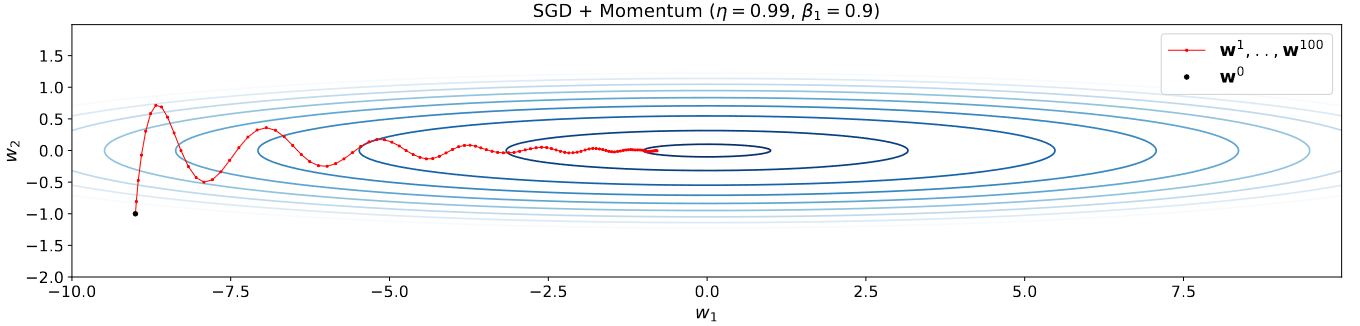
\includegraphics[width=1\textwidth]{assets/pics/sgd-momentum.png}
    \captionsource{Ilustrasi dari pembaruan parameter $\bm{\theta}=\{w_1, w_2\}$ dengan \f{stochastic gradient descent} dengan momentum.}{\citep{geiger2022deeplearning}.}
    \label{fig:sgd-momentum}
\end{figure}

Metode lainnya yang dapat digunakan untuk mempercepat proses pembaruan parameter $\bm{\theta}$ adalah metode \f{adaptive learning rate}. Metode \f{adaptive learning rate} mengubah \f{learning rate} pada setiap parameter $\bm{\theta}$ dengan membagi \f{learning rate} awal dengan \f{moving average} dari kuadrat gradien -- biasanya disebut sebagai \f{running variance} -- pada parameter $\bm{\theta}$ tersebut. Pembagian antara gradien dan \f{running variance} tersebut dilakukan secara \f{element-wise}. \equ~\ref{eq:rmsprop} menunjukkan algoritma \f{stochastic gradient descent} dengan \f{adaptive learning rate} dan \pic~\ref{fig:rmsprop} menngilustrasikan pembaruan parameter $\bm{\theta}$ dengan \f{adaptive learning rate}.
\begin{align}
    \label{eq:rmsprop}
    \bm{\theta}^{(t+1)} &= \bm{\theta}^{(t)} - \frac{\eta \nabla_{\bm{\theta}} L_{\mathcal{B}}(\bm{\theta}^{(t)})}{\sqrt{\mathbf{v}^{(t+1)}} + \epsilon}, \\
    \mathbf{v}^{(t+1)} &= \beta_2 \mathbf{v}^{(t)} + (1 - \beta_2) \left(\nabla_{\bm{\theta}} L_{\mathcal{B}}(\bm{\theta}^{(t)})\odot \nabla_{\bm{\theta}} L_{\mathcal{B}}(\bm{\theta}^{(t)})\right),
\end{align}
dengan $\beta_2 \in [0, 1)$ dan $\odot$ adalah operasi perkalian \f{element-wise} antara dua matriks atau vektor.
\begin{figure}
    \centering
    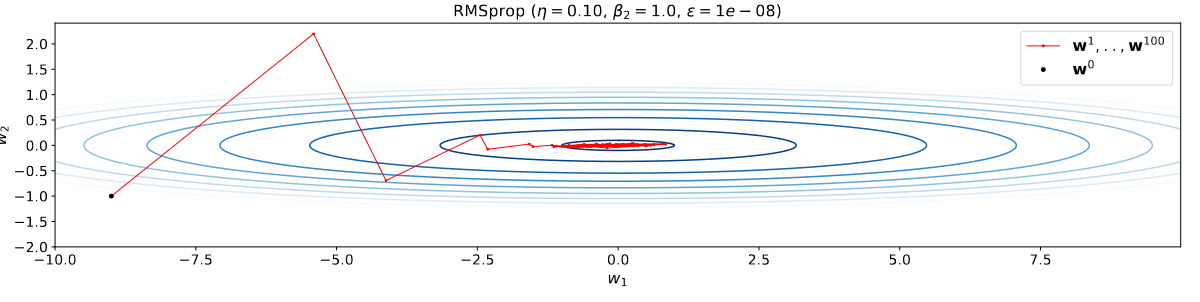
\includegraphics[width=1\textwidth]{assets/pics/RMSPROP.png}
    \captionsource{Ilustrasi dari pembaruan parameter $\bm{\theta}=\{w_1, w_2\}$ dengan \f{adaptive learning rate}.}{\citep{geiger2022deeplearning}.}
    \label{fig:rmsprop}
\end{figure}

Faktor $\epsilon$ yang ditambahkan pada \equ~\ref{eq:rmsprop} digunakan untuk menghindari pembagian dengan nol pada awal iterasi karena inisialiasi awal vektor $\mathbf{v}^{(0)}$ adalah nol.

Terakhir, metode optimasi \f{Adaptive Moment Estimation} (Adam) menggabungkan metode \f{stochastic gradient descent} dengan momentum dan \f{adaptive learning rate}. \equ~\ref{eq:adam} menunjukkan algoritma \f{stochastic gradient descent} dengan Adam dan \pic~\ref{fig:adam} mengilustrasikan pembaruan parameter $\bm{\theta}$ dengan Adam. \equ~\ref{eq:adam} menunjukkan persamaan dari metode optimasi Adam dan \pic~\ref{fig:adam} mengilustrasikan pembaruan parameter $\bm{\theta}$ dengan Adam.
\begin{figure}
    \centering
    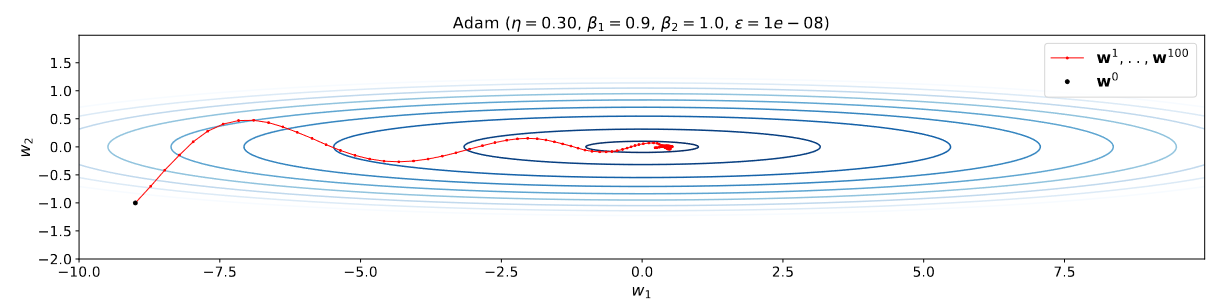
\includegraphics[width=1\textwidth]{assets/pics/adam.png}
    \captionsource{Ilustrasi dari pembaruan parameter $\bm{\theta} = \{w_1, w_2\}$ dengan Adam.}{\citep{geiger2022deeplearning}.}
    \label{fig:adam}
\end{figure}
\begin{align}
    \label{eq:adam}
    \bm{\theta}^{(t+1)} &= \bm{\theta}^{(t)} - \frac{\eta \hat{\mathbf{m}}^{(t+1)}}{\sqrt{\hat{\mathbf{v}}^{(t+1)}} + \epsilon}, \\
    \label{eq:adam-momemntum-with-bias-correction}
    \hat{\mathbf{m}}^{(t+1)} &= \frac{\mathbf{m}^{(t+1)}}{1 - \beta_1}, \\
    \label{eq:adam-running-variance-with-bias-correction}
    \hat{\mathbf{v}}^{(t+1)} &= \frac{\mathbf{v}^{(t+1)}}{1 - \beta_2}, \\
    \mathbf{m}^{(t+1)} &= \beta_1 \mathbf{m}^{(t)} + (1 - \beta_1) \nabla_{\bm{\theta}} L_{\mathcal{B}}(\bm{\theta}^{(t)}), \\
    \mathbf{v}^{(t+1)} &= \beta_2 \mathbf{v}^{(t)} + (1 - \beta_2) \left(\nabla_{\bm{\theta}} L_{\mathcal{B}}(\bm{\theta}^{(t)})\odot \nabla_{\bm{\theta}} L_{\mathcal{B}}(\bm{\theta}^{(t)})\right).
\end{align}

Alasan dilakukan pembagian dengan $(1-\beta_1)$ dan $(1-\beta_2)$ \equ~\ref{eq:adam-momemntum-with-bias-correction} dan \equ~\ref{eq:adam-running-variance-with-bias-correction} adalah untuk menghilangkan bias pada \f{momentum} dan \f{running variance} pada awal iterasi.


\section{Pembelajaran Representasi}
Pembelajaran representasi adalah proses pembelajaran model \f{machine learning} atau \f{deep learning} $f_{\text{model}}(x): \mathcal{X} \rightarrow \mathbb{R}^n$ yang memetakan \f{high dimensional input} $x \in \mathcal{X}$ ke dalam ruang vektor $\mathbb{R}^n$. Pemetaan yang diharapkan dari model $f_{\text{model}}(x)$ diharapkan dapat mengenkode informasi yang terkandung pada $x$ ke dalam vektor $\mathbf{R}^n$. Salah satu contoh informasi yang dapat dienkode adalah jarak antara dua kalimat $x_1$ dan $x_2$ yang memiliki kesamaan semantik atau sintaksis akan lebih dekat daripada jarak antara dua kalimat $x_1$ dan $x_3$ yang tidak memiliki kesamaan sama sekali pada ruang vektor. \pic~\ref{fig:reps-learning} mengilustrasikan pemetaan \f{input} menjadi vektor.
\begin{figure}
    \centering
    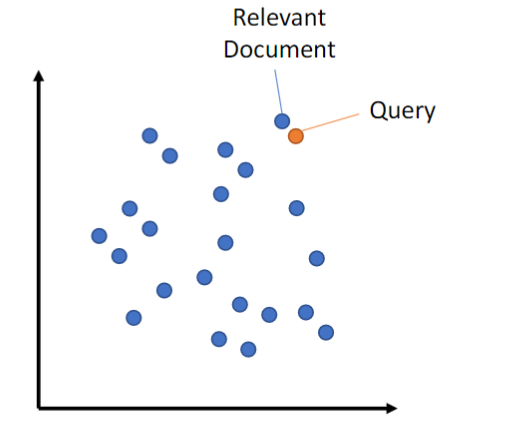
\includegraphics[width=0.5\textwidth]{assets/pics/reps-learning.png}
    \captionsource{Ilustrasi dari Pemetaan \f{input} menjadi vektor. \f{input} yang memiliki kesamaan semantik atau sintaksis akan lebih dekat daripada \f{input} yang tidak memiliki kesamaan.}{\url{https://www.sbert.net}}
    \label{fig:reps-learning}
\end{figure}

\subsection{Fungsi \f{Loss} pada Pembelajaran Representasi}


Fungsi loss pada pembelajaran representasi untuk permasalahan pemeringkatan teks biasanya disebut sebagai \f{ranking loss}. Meminimalkan fungsi \f{ranking loss} berarti memastikan bahwa \f{input-input} yang serupa berada lebih dekat daripada \f{input-input} yang tidak mirip. Sebagian besar fungsi loss pada pembelajaran representasi tidak memerlukan label kelas.

Fungsi loss yang digunakan pada penelitian ini adalah \f{N-pair loss} \citep{InfoNCE}. \f{N-pair loss} dapat ditinjau sebagai klasifikasi multikelas dengan N-1 kelas berupa kelas negatif (kelas yang tidak mirip dengan \f{input} yang diberikan) dan 1 kelas positif (kelas yang mirip dengan \f{input} yang diberikan). Untuk suatu \f{input} $x$ dan \f{input} positif $x^+$ dan kumpulan \f{input} negatif $\{x^-_i\}_{i=1}^{N-1}$, \f{N-pair loss} dapat ditulis seperti pada \equ~\ref{eq:n-pair-loss}.
\begin{align}
\label{eq:n-pair-loss}
\nonumber
 L(x, x^+, \{x^-_i\}_{i=1}^{N-1}) = \\
 -\log\frac{\exp(\text{sim}((f_\text{model}(x), f_\text{model}(x^+)))}{\sum_{i=1}^{N-1} \exp(\text{sim}(f_\text{model}(x), f_\text{model}(x^-_i)))+\exp(\text{sim}(f_\text{model}(x), f_\text{model}(x^+)))},
\end{align}
dengan $\text{sim}$ adalah fungsi yang mengukur keserupaan antara dua vektor (fungsi jarak). Pada penelitian ini, fungsi $\text{sim}$ yang digunakan adalah fungsi \f{dot product} sehingga \equ~\ref{eq:n-pair-loss} dapat ditulis ulang seperti pada \equ~\ref{eq:n-pair-loss-dot-product}.
\begin{align}
\label{eq:n-pair-loss-dot-product}
 L(x, x^+, \{x^-_i\}_{i=1}^{N-1}) &= -\log\frac{\exp(f_\text{model}(x)^{\top}f_\text{model}(x^+))}{\sum_{i=1}^{N-1} \exp(f_\text{model}(x)^{\top}f_\text{model}(x^-_i))+\exp(f_\text{model}(x)^{\top}f_\text{model}(x^+))}.
\end{align}

\pic~\ref{fig:n-pair-loss} mengilustrasikan fungsi \f{N-pair loss}. Untuk pasangan teks yang relevan $(a, b_1)$, tujuannya adalah untuk meminimalkan jarak (fungsi sim) antara $a$ dan $b_1$ sehingga jarak tersebut lebih kecil dibandingkan dengan jarak antara $a$ dan $b_i$ yang lain.
\begin{figure}
    \centering
    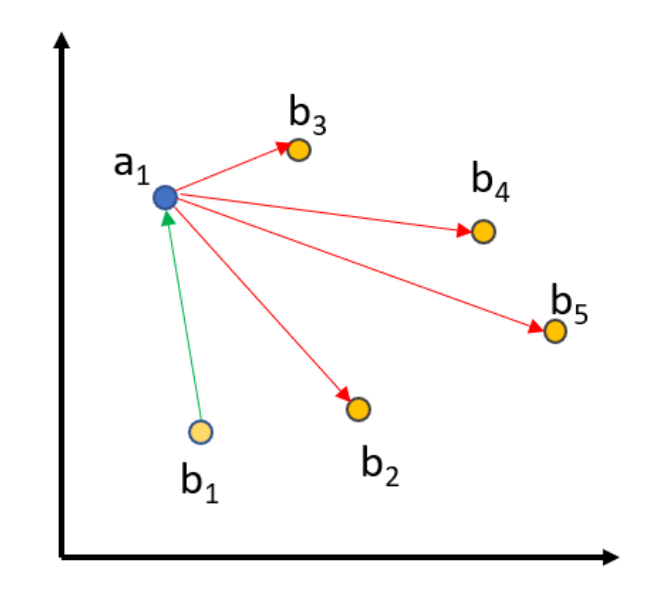
\includegraphics[width=0.5\textwidth]{assets/pics/InfoNCE.png}
    \captionsource{Ilustrasi fungsi objektif \f{N-pair loss}. Untuk pasangan teks yang relevan $(a, b_1)$, tujuannya adalah untuk meminimalkan jarak antara $a$ dan $b_1$ sehingga jarak tersebut lebih kecil dibandingkan dengan jarak antara $a$ dan $b_i$ yang lain.}{\url{https://www.sbert.net/}}
    \label{fig:n-pair-loss}
\end{figure}

















        


\clearchapter
\chapter{\babTiga}
\label{bab:3}

\noindent\todo{
	jabarin sih isinya mau gmna
}

\section{Mekanisme \f{Attention}}
	\subsection{Attention sebagai \f{Dictionary Lookup}}

	Mekanisme \f{Attention} dapat ditinjau sebagai \f{Dictinoary Lookup}, yaitu untuk sebuah vektor kueri $\mathbf{q}$ dan sekumpulan pasangan terurut vektor $\mathcal{KV} = \{(\mathbf{k}_1, \mathbf{v}_2), (\mathbf{k}_2, \mathbf{v}_2), \dots, (\mathbf{k}_n, \mathbf{v}_n)\}$, mekanisme \f{attention} akan mengembalikan vektor nilai $\mathbf{v}_i$ yang memiliki vektor kunci $\mathbf{k}_i$ yang serupa dengan vektor kueri $\mathbf{q}$. \equ~\ref{equ:hard-attention-start} hingga \equ~\ref{equ:hard-attention-end} menunjukkan bagaimana mekanisme \f{attention} dilakukan.

\begin{align}
	\label{equ:hard-attention-start}
	\mathcal{KV} &= \{(\mathbf{k}_1, \mathbf{v}_2), (\mathbf{k}_2, \mathbf{v}_2), \dots, (\mathbf{k}_n, \mathbf{v}_n)\}, \\
	\text{tulis kembali }\mathbf{K}&= \begin{bmatrix}
		\mathbf{k}_1 \\
		\mathbf{k}_2 \\
		\vdots \\
		\mathbf{k}_n
	\end{bmatrix} \in \mathbb{R}^{n \times d_k}, \\
	\mathbf{V} &= \begin{bmatrix}
		\mathbf{v}_1 \\
		\mathbf{v}_2 \\
		\vdots \\
		\mathbf{v}_n
	\end{bmatrix} \in \mathbb{R}^{n \times d_v}, \\
	\text{Attention}(\mathbf{q}, \mathbf{K}, \mathbf{V}) &= \bm{\alpha}\mathbf{V} \in \mathbb{R}^{d_v},\\
	\bm{\alpha} &= [\alpha_{1}, \alpha_{2}, \dots, \alpha_{n}], \\
	\label{equ:hard-attention-end}
	\text{dengan } \alpha_i &= 
	\begin{cases}
	1, & \text{jika } i = \arg\max_{j} f_{attn}(\mathbf{q}, \mathbf{k}_j) \\
	0, & \text{lainnya}
	\end{cases}.
	\end{align}

	$f_{attn}(\mathbf{q}, \mathbf{k})$ adalah fungsi yang menghitung nilai keserupaan antara vektor kueri $\mathbf{q}$ dan vektor kunci $\mathbf{k}$. $\alpha_i$ pada persamaan di atas disebut sebagai bobot atensi dan nilai $f_{attn}(\mathbf{q}, \mathbf{k})$ disebut sebagai nilai atensi.

	Sebagai contoh, untuk $\mathbf{q}= [1,2]$, $\mathcal{KV} = \{([2,1],[1,0]), ([1,2],[0,1])\}$ serta fungsi $f_\text{attn}(\mathbf{q}, \mathbf{k}) =\mathbf{q}\cdot \mathbf{k}$, nilai dari $\text{Attention}( \mathbf{q}, \mathbf{K}, \mathbf{V})$ adalah $[0,1]$, karena nilai maksimal $f_\text{attn}$ terjadi ketika $\mathbf{k} = [1,2]$. 

	Mekansime \f{attention} pada \equ~\ref{equ:hard-attention-start} hingga \equ~\ref{equ:hard-attention-end} disebut sebagai \f{hard attention} karena hanya satu vektor nilai $\mathbf{v}_i$ yang dipilih dari sekumpulan vektor nilai $\mathbf{V}$. Berbeda dengan \f{hard attention} yang tidak terturunkan, \f{soft attention} mengambil seluruh vektor nilai $\mathbf{V}$ dan menghitung bobot $\alpha_i$ untuk setiap vektor nilai $\mathbf{v}_i$ dengan fungsi \f{softmax}. Hasil dari \f{soft attention} adalah rata-rata terbobot dari seluruh vektor nilai $\mathbf{V}$. \equ~\ref{equ:soft-attention-start} dan \pic~\ref{fig:soft-attention} menunjukkan bagaimana \f{soft attention} dilakukan.

	\begin{figure}
		\centering
		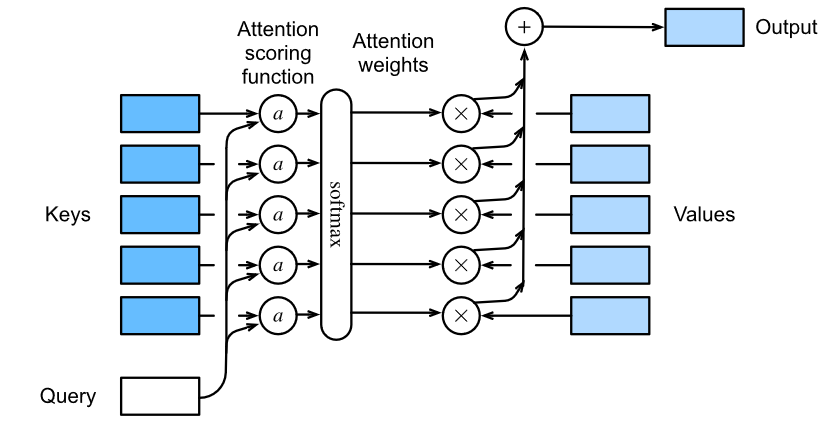
\includegraphics[width=1\textwidth]{assets/pics/softattention.png}
		\caption{Ilustrasi dari mekanisme \f{soft attention} \citep{zhang2023dive}}
		\label{fig:soft-attention}
	\end{figure}

	\begin{align}
		\label{equ:soft-attention-start}
		\text{Attention}(\mathbf{q}, \mathbf{K}, \mathbf{V}) &= \mathbf{\alpha}\mathbf{V} \in \mathbb{R}^{d_v},\\
		\text{dengan } \bm{\alpha} &= [\alpha_{1}, \alpha_{2}, \dots, \alpha_{n}], \\
		\text{dan } \alpha_{i}(\mathbf{q},\mathbf{k}_i) &= \text{Softmax}_i(\bm{\alpha}) = \frac{\exp(f_{attn}(\mathbf{q}, \mathbf{k}_i))}{\sum_{j=1}^{n} \exp(f_{attn}(\mathbf{q}, \mathbf{k}_j))}, \\
		\sum_{i=1}^{n} \alpha_{i} &= 1, \\
		\label{equ:soft-attention-end}
		0 \leq \alpha_{i} &\leq 1.
	\end{align}

	Dengan rata-rata terbobot dari $\mathbf{V}$, \f{soft attention} dapat dicari turunannya dengan \f{backpropagation} yang merupakan syarat \f{fundamental} yang harus dimiliki oleh sebuah model \f{deep learning}.

	Untuk contoh yang serupa dengan \f{hard attention},hasil dari $\text{Attention}(\mathbf{q}, \mathbf{K}, \mathbf{V})$ adalah $0.268 [1,0] + 0.732 [0,1] = [0.732, 0.268]$ dengan $\alpha_1 = \frac{\exp(4)}{\exp(4) + \exp(5)} \approx 0.268$ dan $\alpha_2 = \frac{\exp(5)}{\exp(4) + \exp(5)} \approx 0.732$.

	Pada kasus kumpulan kueri $\mathcal{Q} = \{\mathbf{q}_1, \mathbf{q}_2, \dots, \mathbf{q}_m\}$, Perhitungan atensi untuk setiap triplet $(\mathbf{q}_i, \mathbf{K}, \mathbf{V})$ dapat dihitung secara bersamaan dengan menggunakan operasi matriks. \equ~\ref{equ:soft-attention-start} hingga \equ~\ref{equ:soft-attention-end} yang digunakan untuk kasus 1 kueri dapat ditulis ulang seperti pada \equ~\ref{equ:soft-attention-matrix-start} hingga \equ~\ref{equ:soft-attention-matrix-end}.

	\begin{align}
		\label{equ:soft-attention-matrix-start}
		\text{tulis }\mathbf{Q} &= \begin{bmatrix}
			\mathbf{q}_1 \\
			\mathbf{q}_2 \\
			\vdots \\
			\mathbf{q}_m
		\end{bmatrix} \in \mathbb{R}^{m \times d_k}, \\
		\text{Attention}(\mathbf{Q}, \mathbf{K}, \mathbf{V}) &= \mathbf{A} \mathbf{V} \in \mathbb{R}^{m \times d_v},\\
		\mathbf{A} &= \begin{bmatrix}
			\bm{\alpha}_1 \\
			\bm{\alpha}_2 \\
			\vdots \\
			\bm{\alpha}_m
		\end{bmatrix} = \begin{bmatrix}
			\alpha_{11} & \alpha_{12} & \dots & \alpha_{1n} \\
			\alpha_{21} & \alpha_{22} & \dots & \alpha_{2n} \\
			\vdots & \vdots & \ddots & \vdots \\
			\alpha_{m1} & \alpha_{m2} & \dots & \alpha_{mn} \\
		\end{bmatrix} \in \mathbb{R}^{m \times n}, \\
		\label{equ:soft-attention-matrix-end}
		\alpha_{ij}(\mathbf{q}_i, \mathbf{k}_j) &= \text{Softmax}_j(\mathbf{\alpha}_i) = \frac{\exp(f_{attn}(\mathbf{q}_i, \mathbf{k}_j))}{\sum_{k=1}^{n} \exp(f_{attn}(\mathbf{q}_i, \mathbf{k}_k))},
	\end{align}

	dengan $\alpha_{ij}$ adalah bobot yang menunjukkan bobot atensi antara vektor kueri $\mathbf{q}_i$ dengan vektor kunci $\mathbf{k_j}$. 

	\subsection{Regresi Kernel Sebagai \f{Attention} non-parametrik}
	\label{sec:regresi-kernel}

	Salah satu pengunaan mekanisme \f{attention} terdapat pada regresi kernel, yang merupakan model statistik non-parametrik. \f{Attention} berubah menjadi regresi kernel dengan memilih fungsi keserupaan $f_{attn}(\mathbf{q}, \mathbf{k})$ menjadi fungsi non-parametrik $\mathcal{K}(\mathbf{q}, \mathbf{k})$, dan mengganti fungsi softmax menjadi fungsi normalisasi standar, seperti pada \equ~\ref{equ:regresi-kernel-end}.
	
	Pada model non-parametrik, model yang dibangun tidak memiliki parameter yang harus diestimasi atau dipelajari, melainkan model non-parametrik menggunakan seluruh atau sebagian dari \f{datasets} latih $\mathcal{D} = \{(\mathbf{x}_1, y_1), (\mathbf{x}_2, y_2), \dots, (\mathbf{x}_n, y_n)\}$ untuk memberikan prediksi $y_*$ untuk sebuah data uji $\mathbf{x}_*$. \equ~\ref{equ:regresi-kernel-start} hingga \equ~\ref{equ:regresi-kernel-end} menunjukkan bagaimana model regresi kernel melakukan prediksi $y_*$ untuk sebuah data uji $\mathbf{x}_*$.

	\begin{align}
		\label{equ:regresi-kernel-start}
		y_{*} = f(\mathbf{x}_{*}) &= \sum_{i=1}^{n} \alpha_{i}(\mathbf{x}_{*},\mathbf{x}_i) y_i, \\
		\label{equ:regresi-kernel-end}
		\text{dengan } \alpha_{i}(\mathbf{x}_{*},\mathbf{x}_i) &= \frac{\mathcal{K}(\mathbf{x}_{*},\mathbf{x}_i)}{\sum_{j=1}^{n} \mathcal{K}(\mathbf{x}_{*},\mathbf{x}_j)} \in [0, 1].
	\end{align}

	$\mathcal{K}(\mathbf{x}_{*},\mathbf{x}_i)$ adalah fungsi kernel (non-parametrik) yang menghitung keserupaan antara data uji $\mathbf{x}_{*}$ dengan data latih $\mathbf{x}_i$. \equ~\ref{equ:regresi-kernel-end} merupakan bentuk khusus dari mekansime \f{soft attention} \equ~\ref{equ:soft-attention-start}, dengan kueri $\mathbf{q}$ adalah data uji $\mathbf{x}_{*}$, kunci $\mathbf{k}_i$ adalah data latih $\mathbf{x}_i$, nilai $\mathbf{v}_i$ adalah $y_i$. \equ~\ref{equ:regresi-kernel-gaussian-start} menujukkan contoh kernel regresi dengan pemilihan kernel Gaussian $\mathcal{K}(\mathbf{x}_{*},\mathbf{x}_i) = \exp(-\frac{||\mathbf{x}_{*} - \mathbf{x}_i||^2 \beta}{2})$.

	\begin{align}
		\label{equ:regresi-kernel-gaussian-start}
		y_{*} = f(\mathbf{x}_{*}) &= \sum_{i=1}^{n} \alpha_{i}(\mathbf{x}_{*},\mathbf{x}_i) y_i	\\
		&= \sum_{i=1}^{n} \frac{\exp\left(-\frac{||\mathbf{x}_{*}-\mathbf{x}_i||^2 \beta^2}{2}\right)}{\sum_{j=1}^{n} \exp\left(-\frac{||\mathbf{x}_{*}-\mathbf{x}_j||^2 \beta^2}{2}\right)} y_i
	\end{align}

	\subsection{\f{Attention} Parametrik}

	Mekanisme \f{attention} yang dilakukan oleh \cite{transformerori} merupakan mekanisme \f{attention} parametrik. Salah satu alasan penggunaan $f_{attn}$ yang parametrik adalah pemilihan fungsi $f_{attn}$ yang non-parametrik seperti pada \sect~\ref{sec:regresi-kernel} memiliki kelemahan:


	\begin{enumerate}
		\item Relasi antar vektor kueri $\mathbf{q}$ dan vektor kunci $\mathbf{k}$ harus diketahui sebelumnya untuk memilih fungsi $f_{attn}$ yang tepat.
		\item Prediksi $y_*$ memerlukan seluruh data latih $\mathcal{D}$, $O(|\mathcal{D}|)$ komputasi diperlukan untuk melakukan satu prediksi.
	\end{enumerate}

	

	Pada mekanisme \f{attention} parametrik, nilai vektor kueri $\mathbf{q}$ dan $\mathbf{v}$ dibandingkan pada ruang vektor yang akan dipelajari (\f{learned embedding space}) daripada ruang vektor aslinya. Sebagai contoh, untuk suatu kueri $\mathbf{q}\in \mathbb{R}^{d_q}$, dan vektor kunci $\mathbf{k} \in \mathbb{R}^{d_k}$, \f{additive attention} yang diperkenalkan oleh \cite{bahdanau2016neural} menghitung nilai keserupaan antara $\mathbf{q}$ dan $\mathbf{k}$ seperti pada \equ~\ref{equ:additive-attention}

	\begin{align}
	\label{equ:additive-attention}
	f_{attn}(\mathbf{q} \mathbf{W}^q, \mathbf{k} \mathbf{W}^k) &= (\mathbf{q} \mathbf{W}^q  + \mathbf{k} \mathbf{W}^k)  \mathbf{W}^{\text{out}} \in \mathbb{R}, \\
	\text{dengan } &\mathbf{W}^q \in \mathbb{R}^{d_q \times d_{\text{attn}}}, \mathbf{W}^k \in \mathbb{R}^{d_k \times d_{\text{attn}}}, \mathbf{W}_{\text{out}} \in \mathbb{R}^{d_{\text{attn}} \times 1},
	\end{align}

	Dengan $\mathbf{W}^q$, $\mathbf{W}^k$, dan $\mathbf{W}^{\text{out}}$ adalah matriks parameter bobot yang akan diestimasi atau dipelajari selama proses pelatihan. Contoh parametrik \f{attention} yang lebih sederhana adalah \f{dot-product attention}. Fungsi $f_{attn}$ yang digunakan adalah perkalian titik antara $\mathbf{q}$ dan $\mathbf{k}$ di ruang vektor yang dipelajari (\f{learned embedding space}). \equ~\ref{equ:dot-product-attention} menunjukkan bagaimana \f{dot-product attention} dihitung.

	\begin{align}
		\label{equ:dot-product-attention}
		f_{attn}(\mathbf{q} \mathbf{W}^q, \mathbf{k} \mathbf{W}^k) = (\mathbf{q} \mathbf{W}^q) (\mathbf{k} \mathbf{W}^k)^{\top}\\
		\text{dengan } \mathbf{W}^q \in \mathbb{R}^{d_q \times d_{\text{attn}}}, \mathbf{W}^k \in \mathbb{R}^{d_k \times d_{\text{attn}}}.
	\end{align}

\section{Transformer}


	\begin{figure}
		\centering
		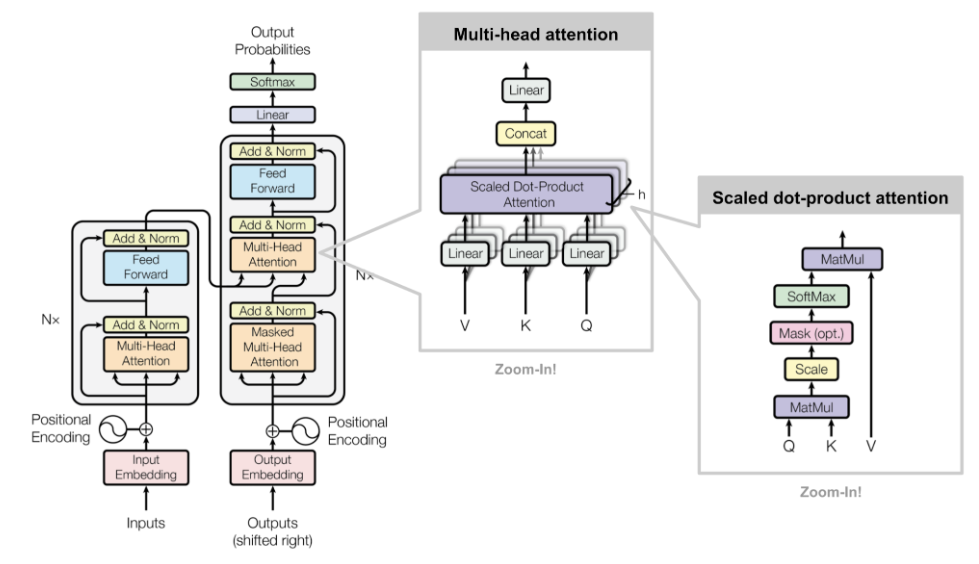
\includegraphics[width=1\textwidth]{assets/pics/lilianweng-transformer.png}
		\caption{Arsitektur \f{transformer} \citep{weng2018attention}.}
		\label{fig:transformer}
	\end{figure}

	\f{Transformers} merupakan Arsitektur \f{deep learning} yang pertama kali diperkenalkan oleh \cite{transformerori}. Awalnya Transformers merupakan model \f{sequance to sequance} yang diperuntukkan untuk permasalahan mesin translasi neural (\f{neural machine translation}). Namun, sekarang \f{transformer} juga digunakan untuk permasalahan pemrosesan bahasa alami lainnya. model-model yang berarsitektur \f{transformer} menjadi model \f{state-of-the-art} untuk permasalahan pemrosesan bahasa alami lainnya, seperti \f{question answering}, \f{sentiment analysis}, dan \f{named entity recognition}.
 
	Berbeda dengan arsitektur mesin translasi terdahulu, transformer tidak mengunakan \f{recurrent neural network} (RNN) atau \f{convolutional neural network} (CNN), melainkan transformer adalah model \f{feed foward network} yang dapat memproses seluruh \f{input} pada barisan secara paralel. Untuk menggantikan kemampuan RNN dalam mempelajari ketergantungan antar \f{input} yang berurutan dan kemampuan CNN dalam mempelajari fitur lokal, transformer bergantung pada mekanisme \f{attention}.

	Terdapat tiga jenis \f{attention} yang digunakan dalam model \f{transformer} \citep{transformerori}:
	\begin{enumerate}
		\item \f{Encoder self-attention}: menggunakan barisan \f{input} yang berupa barisan token atau kata sebagai masukan untuk menghasilkan barisan representasi kontekstual, berupa vektor, dari \f{input}. Setiap representasi token tersebut memiliki ketergantungan dengan token lainnya dari barisan \f{input}.
		\item \f{Decoder self-attention}: menggunakan barisan \f{target} yang berupa kalimat terjemahan parsial, barisan token, sebagai masukan untuk menghasilkan barisan representasi kontekstual (vektor) dari \f{target}. Setiap representasi token tersebut memiliki ketergantungan dengan token sebelumnya dalam urutan masukan.
		\item \f{Decoder-encoder attention}: menggunakan barisan representasi kontekstual dari \f{input}, dan barisan representasi kontekstual dari \f{target} untuk menghasilkan token berikutnya yang merupakan hasil prediksi dari model. Barisan \f{target} yang digabung dengan token hasil prediksi tersebut akan menjadi barisan \f{target} untuk prediksi selanjutnya.
	\end{enumerate}

	Arsitektur dari \f{transformer} mengimplementasikan struktur pasangan encoder-decoder. Aristektur dari \f{transformer} dapat dilihat pada \pic~\ref{fig:transformer}. Lapisan\f{encoder} berfungsi untuk memahami konteks suatu kata dalam dokumen atau kalimat, sementara lapisan \f{decoder} digunakan untuk menyelesaikan masalah translasi menuju bahasa berbeda. \sect~\ref{sec:token-embedding} hingga \sect~\ref{sec:encoder} menjelaskan arsitektur model \f{transformer} dan berbagai mekanisme yang menyusun model \f{transformer}, khususnya \f{transformer encoder} yang menjadi \f{building block} dari \f{Biderectional Encoder Representations from Transformers} (BERT).

	\subsection{\f{Token Embedding (Input Embedding)}}
	\label{sec:token-embedding}

	\begin{figure}
		\centering
		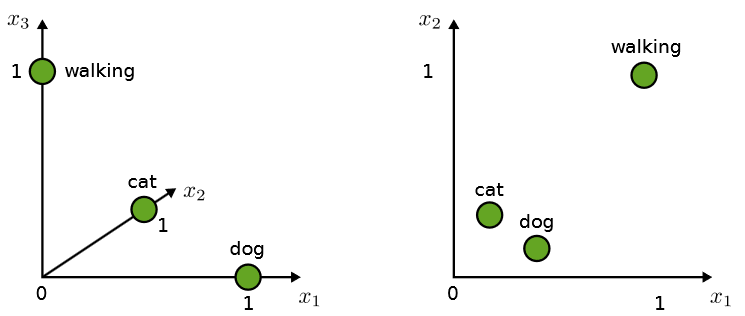
\includegraphics[width=1\textwidth]{assets/pics/token-embedding.png}
		\caption{Ilustrasi dari representasi token. Gambar kiri menunjukkan representasi token dengan \f{one-hot encoding}, sedangkan gambar kanan menunjukkan representasi token dengan \f{token embedding} \citep{geiger2022deeplearning}}
		\label{fig:token-embedding}
	\end{figure}

	Perlu diingat kembali bahwa \f{input} dari \f{Attention} (dan tentunya \f{transformer}) adalah barisan vektor. Jika \f{Attention} ingin dapat digunakan pada permasalahan bahasa, barisan kata atau subkata (selanjutnya disebut token) harus terlebih dahulu diubah menjadi barisan vektor.

	Representasi vektor dari token yang paling sederhana adalah dengan \f{one-hot encoding}. Andaikan $\mathcal{T} = \{t_1, t_2, \dots, t_{|\mathcal{T}|}\}$ adalah semua kemungkinan token yang mungkin muncul dalam permasalahan bahasa yang ingin diselesaikan. Untuk sembarang barisan token $t = (t_{i_1}, t_{i_2}, \dots, t_{i_L})$, representasi vektor dari token $t_{i_j}$ adalah vektor $\mathbf{oh}_{i_j} = [0, \dots, 0, 1, 0, \dots, 0] \in \mathbb{R}^{|\mathcal{T}|}$, dengan nilai 1 pada indeks ke $j$ dan nilai 0 pada indeks lainnya. \f{One-hot encoding} tentunya memiliki kelemahan:

	\begin{enumerate}
		\item Vektor yang dihasilkan adalah \f{sparse vector}, dan ukuran vektor yang dihasilkan cukup besar, yaitu $|\mathcal{T}|$.
		\item Representasi token yang buruk. Operasi vektor yang dilakukan pada \f{one-hot encoding} tidaklah bermakna. Misalnya, Jarak antar token akan selalu sama pada \f{one-hot encoding}, yaitu $\sqrt{2}$.
	\end{enumerate}

	Untuk Mengatasi kekurangan dari representasi \f{one-hot encoding}, reprentasi yang digunakan adalah vektor padat yang akan dipelajari ketika proses pelatihan. Misalkan $\mathbf{E}_{\mathcal{T}} \in \mathbb{R}^{|\mathcal{T}| \times d_{\text{token}}}$ adalah matriks parameter yang merupakan representasi vektor padat dari seluruh token ada. \equ~\ref{equ:token-embedding-start} hingga \equ~\ref{equ:token-embedding-end} menunjukkan bagaimana representasi vektor dari barisan suatu token $t$ dihitung. 

	\begin{align}
		\label{equ:token-embedding-start}
		t &= (t_{i_1}, t_{i_2}, \dots, t_{i_L}), \\
		\mathbf{e}_{i_j} &= \mathbf{oh}_{i_j} \mathbf{E}_{\mathcal{T}} \in \mathbb{R}^{d_{\text{token}}}, \\
		\label{equ:token-embedding-end}
		\text{Embed}(t) &= \mathbf{E}_{t} = \begin{bmatrix}
			\mathbf{e}_{i_1} \\
			\mathbf{e}_{i_2} \\
			\vdots \\
			\mathbf{e}_{i_L}
		\end{bmatrix} \in \mathbb{R}^{L \times d_{\text{token}}}.
	\end{align}

	\subsection{\f{Scaled Dot-Product Attention}}
	\label{sec:scaled-dot-product-attention}
	\f{Scaled dot-product attention} adalah mekanisme \f{Attention} parametrik yang digunakan dalam \f{transformers}. \f{Scaled dot-product attention} menghitung keserupaan antara vektor kueri $\mathbf{q}$ dan vektor kunci $\mathbf{k}$ pada ruang vektor yang dipelajari (\f{learned embedding space}) dengan fungsi keserupaan $f_{attn}(\mathbf{q} \mathbf{W}^q, \mathbf{k}\mathbf{W}^k) $ adalah perkalian titik antara $\mathbf{qW}^q$ dan $\mathbf{kW}^k$ yang kemudian dibagi dengan $\sqrt{d_{attn}}$, seperti pada \equ~\ref{equ:scaled-dot-product-attention}.

	\begin{align}
		\label{equ:scaled-dot-product-attention}
		f_{attn}(\mathbf{q} \mathbf{W}^q, \mathbf{k} \mathbf{W}^k) &= \frac{\mathbf{q} \mathbf{W}^q (\mathbf{k} \mathbf{W}^k)^{\top}}{\sqrt{d_{attn}}} \in \mathbb{R}, \\
		\text{dengan } &\mathbf{W}^q \in \mathbb{R}^{d_q \times d_{\text{attn}}}, \mathbf{W}^k \in \mathbb{R}^{d_k \times d_{\text{attn}}}.
	\end{align}

	pembagian dengan $\sqrt{d_{attn}}$ dilakukan untuk menjaga variansi dari nilai atensi $\mathbf{q} \mathbf{W}^q (\mathbf{k} \mathbf{W}^k)^{\top}$ tetap serupa dengan variansi $\mathbf{qW}^q$ dan $\mathbf{kW}^k$. Tanpa pembagian $\sqrt{d_{attn}}$, variansi dari nilai atensi akan memiliki faktor tambahan $\sigma^2 d_{attn}$, seperti yang ditunjukkan pada \equ~\ref{equ:initialize-dot-product-attention} hingga \equ~\ref{equ:variance-dot-product-attention}.

	\begin{align}
		\label{equ:initialize-dot-product-attention}
		\mathbf{qW}^q \sim \mathcal{N}(0, \sigma^2) \text{ dan } \mathbf{kW}^k \sim \mathcal{N}(0, \sigma^2). \\
		\label{equ:variance-dot-product-attention}
		\text{Var}(\mathbf{qW}^q (\mathbf{kW}^k)^{\top}) = \sum_{i=1}^{d_{attn}} \text{Var}\left((\mathbf{qW}^q)_i ((\mathbf{kW}^k)^{\top}_i\right) = \sigma^4 d_{attn}.
	\end{align}
	
	Akibatnya, untuk nilai $d_{attn}$ yang cukup besar, akan terdapat satu elemen atensi acak $(\mathbf{qW}^q (\mathbf{kW}^k)^{\top})_i$ sehinnga $(\mathbf{qW}^q (\mathbf{kW}^k)^{\top})_i \gg (\mathbf{qW}^q (\mathbf{kW}^k)^{\top})_j$ untuk sembarang nilai atensi lainnya. Jika faktor $d_{attn}$ tidak dihilangkan, \f{softmax} dari nilai atensi akan jenuh ke 1 untuk satu elemen acak tersebut dan 0 untuk elemen lainnya. Akibatnya, gradien pada fungsi \f{softmax} akan mendekati nol sehingga model tidak dapat belajar parameter dengan baik. 

	Dengan \f{scaled dot product attention}, tidak ada faktor $d_{attn}$ pada variansi dari nilai atensi. faktor $\sigma^4$ pada \equ~\ref{equ:variance-scaled-dot-product-attention} tidak menjadi masalah karena inisialisasi bobot Kaiming dan \f{layer normalisasi} yang dijelaskan pada \sect~\ref{sec:kaiminginit} dan \sect~\ref{sec:layer-normalization} mengakibatkan $\sigma^2 \approx 1$ sehingga $\sigma^4 \approx \sigma^2 \approx 1$.

	\begin{align}
		\label{equ:variance-scaled-dot-product-attention}
		\text{(scaled dot product attention) }\text{Var}\left(\frac{\mathbf{qW}^q (\mathbf{kW}^k)^{\top}}{\sqrt{d_{attn}}}\right) = \frac{\sigma^4 d_{attn}}{d_{attn}} = \sigma^4
	\end{align}

	Terakhir, untuk kumpulan vektor kueri $\mathcal{Q} = \{\mathbf{q}_1, \mathbf{q}_2, \dots, \mathbf{q}_m\}$, dan kumpulan vektor kunci dan nilai $\mathcal{KV} = \{(\mathbf{k}_1, \mathbf{v}_2), (\mathbf{k}_2, \mathbf{v}_2), \dots, (\mathbf{k}_n, \mathbf{v}_n)\}$, \f{scaled dot product attention} dapat dihitung secara bersamaan seperti pada \equ~\ref{equ:scaled-dot-product-attention-matrix-start} hingga \equ~\ref{equ:scaled-dot-product-attention-matrix-end}.

	\begin{align}
	\label{equ:scaled-dot-product-attention-matrix-start}
	\text{Tulis Kembali } \mathbf{Q} &= \begin{bmatrix}
		\mathbf{q}_1 \\
		\mathbf{q}_2 \\
		\vdots \\
		\mathbf{q}_m \\
	\end{bmatrix} \in \mathbb{R}^{m \times d_{q}}, \\
	\mathbf{K} &= \begin{bmatrix}
		\mathbf{k}_1 \\
		\mathbf{k}_2 \\
		\vdots \\
		\mathbf{k}_n \\
	\end{bmatrix} \in \mathbb{R}^{n \times d_{k}}, \\
	\text{dan } \mathbf{V} &= \begin{bmatrix}
		\mathbf{v}_1 \\
		\mathbf{v}_2 \\
		\vdots \\
		\mathbf{v}_n \\
	\end{bmatrix} \in \mathbb{R}^{n \times d_{v}}, \\
	\label{equ:scaled-dot-product-attention-matrix-end}
	\text{Attention}(\mathbf{QW}^q, \mathbf{KW}^k, \mathbf{V}) &= \text{Softmax}( \frac{\mathbf{QW}^q (\mathbf{KW}^k)^{\top}}{\sqrt{d_{attn}}}) \mathbf{V} \in \mathbb{R}^{m \times d_{v}}, \\
	\text{dengan } \mathbf{W}^q &\in \mathbb{R}^{d_q \times d_{\text{attn}}}, \mathbf{W}^k \in \mathbb{R}^{d_k \times d_{\text{attn}}}.
	\end{align}

	\subsection{\f{Self-Attention}}
	\begin{figure}
		\centering
		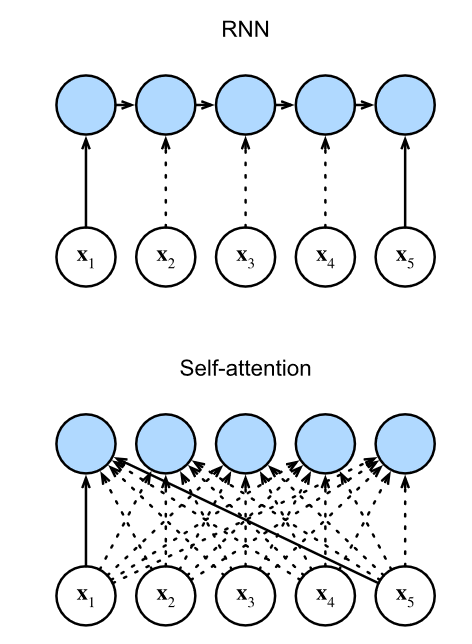
\includegraphics[width=1\textwidth]{assets/pics/rnn-compare-selfattention.png}
		\caption{Perbandingan RNN dan \f{self-attention} dalam menghasilkan representasi vektor kontekstual. Pada RNN, representasi vektor kontekstual setiap token bergantung pada perhitungan token sebelumnya. Pada \f{self-attention}, representasi vektor kontekstual setiap token dihitung secara independen dan paralel.}
		\label{fig:self-attention-rnn}
	\end{figure}

	\begin{figure}
		\centering
		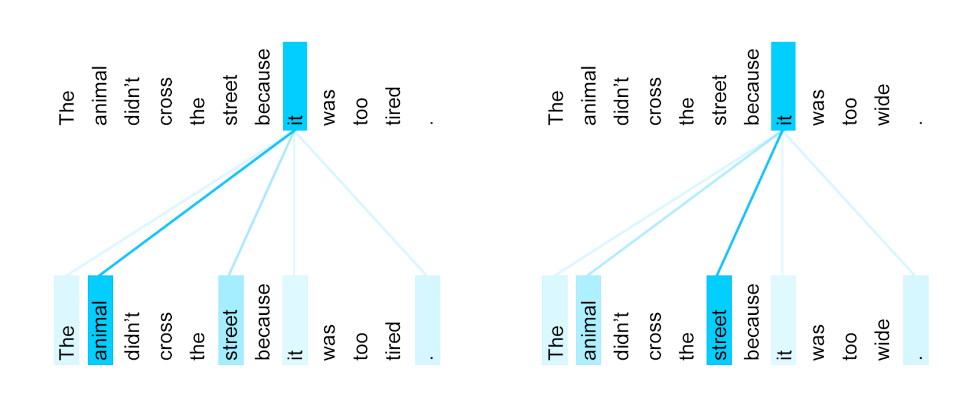
\includegraphics[width=1\textwidth]{assets/pics/self-attn-example.png}
		\caption{Ilustrasi \f{self-attention} dalam menghasilkan representasi vektor kontekstual dari barisan token. Representasi vektor dari token \f{it} akan bergantung terhadap barisan token \f{input}.}
		\label{fig:self-attention-example}
	\end{figure}

	\f{self-Attention layer} adalah layer yang digunakan \f{transformer} untuk menghasilkan representasi vektor yang kontekstual dari barisan token input. Berbeda dengan RNN dalam menghasilkan representasi vektor kontekstual, \f{self-attention} tidak memerlukan ketergantungan sekuensial. Artinya representasi vektor kontekstual setiap tokennya dapat dihitung secara independen dan paralel. \pic~\ref{fig:self-attention-rnn} mengambarkan perbedaan kedua arsitektur dalam menghasilkan representasi vektor kontekstual. Kemampuan Paralelisme dari \f{self-attention} membuat proses komputasi menjadi lebih cepat pada \f{hardware} yang mendukung paralelisme. 

	Perhitungan \f{self-attention} pada \f{transformer} yang digunakan adalah \f{scaled dot product attention} yang telah dijelaskan pada \sect~\ref{sec:scaled-dot-product-attention}. Pada \f{self-attention}, vektor kueri $\mathbf{q}$, vektor kunci $\mathbf{k}$, dan vektor nilai $\mathbf{v}$ adalah vektor yang sama, yaitu \f{embedding} token $\mathbf{E}$ yang dijelaskan pada \sect~\ref{sec:token-embedding}. Selain itu, Dimensi dari \f{learned embedding space} $d_{\text{attn}}$ yang digunakan untuk perhitungan nilai atensi adalah $d_{\text{token}}$ yaitu dimensi dari \f{token embedding}. \equ~\ref{equ:self-attention-start} hingga \equ~\ref{equ:self-attention-end} menunjukkan bagaimana \f{self-attention} dihitung.
	
	
	\begin{align}
		\label{equ:self-attention-start}
		\mathbf{E} &= \text{Embedding dari barisan token} \in \mathbb{R}^{L \times d_{\text{token}}} \\
		\text{Self-Attention}(\mathbf{E}) &= \text{Attention}(\mathbf{EW}^q, \mathbf{EW}^k, \mathbf{EW}^v) \\
		\label{equ:self-attention-end}
		&= \text{Softmax}(\frac{\mathbf{E} \mathbf{W}^q (\mathbf{E} \mathbf{W}^k)^{\top}}{\sqrt{d_{attn}}}) (\mathbf{E} \mathbf{W}^v) \in \mathbb{R}^{L \times d_{\text{token}}} \\
		\text{ dengan } \mathbf{W}^q, \mathbf{W}^k, &\in \mathbb{R}^{d_{\text{token}} \times d_{\text{token}}}, \mathbf{W}^v \in \mathbb{R}^{d_{\text{token}} \times d_{\text{token}}}
	\end{align}

	\f{self-attention} dapat dikonsepsikan sebagai proses pembentukan represenatsi token yang kontekstual. untuk setiap tokennya, \f{self-attention} menghitung keserupaan antara token tersebut ($\mathbf{e}_{t_i} \mathbf{W}^q$) dengan seluruh token lainnya ($\mathbf{E} \mathbf{W}^k$) dengan \f{scaled dot product attention}. Hasil dari \f{scaled dot product attention} adalah vektor yang menunjukkan bobot atensi dari token tersebut terhadap token lainnya. Bobot atensi tersebut kemudian digunakan untuk menghitung rata-rata terbobot dari seluruh token lainnya ($\mathbf{E} \mathbf{W}^v$). Hasil dari rata-rata terbobot tersebut adalah representasi vektor kontekstual dari token tersebut. \pic~\ref{fig:self-attention-example} adalah contoh dari \f{self-attention} yang menghasilkan representasi vektor kontekstual pada token \f{it}. Pada \pic~\ref{fig:self-attention-example} kiri token \f{it} memiliki bobot atensi yang tinggi terhadap token dan \f{animal} sehingga representasi vektor kontekstual dari token \f{it} akan memiliki nilai yang serupa dengan representasi token \f{animal}. Di lain sisi, token \f{it} pada \pic~\ref{fig:self-attention-example} memiliki bobot atensi yang tinggi terhadap token \f{street}.
	
	\subsection{\f{Multi-Head Self-Attention}}

	\begin{figure}
		\centering
		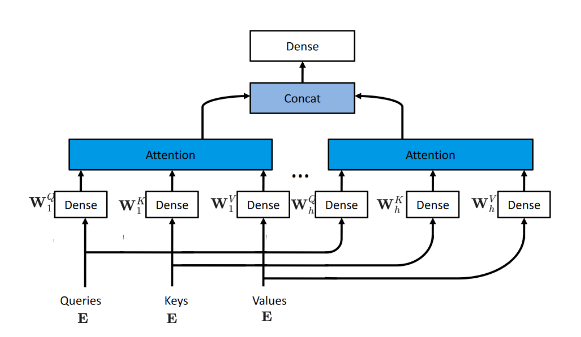
\includegraphics[width=1\textwidth]{assets/pics/MHSA.png}
		\caption{Ilustrasi \f{multi-head self-attention} pada \f{transformer}. \f{Multi-head self-attention} menghitung \f{self-attention} sebanyak $h$ kali pada subruang yang berbeda.}
		\label{fig:multi-head-self-attention}
	\end{figure}

	\f{Multi-Head Self-Attention} adalah arsiktetur pada \f{transformer} untuk melakukan mekanisme \f{self-attention} beberapa kali pada subruang (\f{learned embedded space}) yang berbeda. dengan melakukan hal tersebut, diharapkan bahwa model dapat menangkap relasi atau keserupaan antar token dari sudut pandang yang berbeda. 

	Secara teknis, \f{embedding} dari barisan token $\mathbf{E}$ akan dipetakan sebanyak $h$ kali dengan \f{linear layer} yang kemudian hasil \f{attention} dari setiap \f{head} akan digabungkan dan dilakukan transformasi sekali lagi dengan\f{linear layer}. \equ~\ref{equ:multi-head-self-attention-start} hingga \equ~\ref{equ:multi-head-self-attention-end} menunjukkan bagaimana \f{multi-head self-attention} dihitung.

	\begin{align}
		\label{equ:multi-head-self-attention-start}
		\text{MHSA}(\mathbf{E}) &= \text{Concat}(\text{head}_i, \dots, \text{head}_h)\mathbf{W}^O \in \mathbb{R}^{L \times d_{\text{token}}} \\
		\text{head}_i = \text{Self-Attention}_i(\mathbf{E}) &= \text{Softmax}(\frac{\mathbf{E} \mathbf{W}^q_i (\mathbf{E} \mathbf{W}^k_i)^{\top}}{\sqrt{d_{\text{token}}/h}}) \mathbf{E} \mathbf{W}^v_i  \in  \mathbb{R}^{L \times \frac{d_{\text{token}}}{h}} \\
		\text{Concat}(\text{head}_1, \dots, \text{head}_h) &= [\text{head}_1 | \dots | \text{head}_h] \in \mathbb{R}^{L \times d_{\text{token}}} \\
		\label{equ:multi-head-self-attention-end}
		\text{dengan } \mathbf{W}^q_i, \mathbf{W}^k_i, \mathbf{W}^v_i,&\in \mathbb{R}^{\frac{d_{\text{token}}}{h} \times \frac{d_{\text{token}}}{h}}, \mathbf{W}^O \in \mathbb{R}^{d_{\text{token}} \times d_{\text{token}}} \\	
	\end{align}

	perhatikan bahwa dimensi dari \f{learned embedding space} menjadi $\frac{d_{\text{token}}}{h}$ untuk setiap \f{head}-nya. Hal ini dilakukan untuk menjaga dimensi dari \f{output} terakhir tetap sama dengan dimensi dari \f{input}, yaitu $d_{\text{token}}$. Selain itu, argumen lainnya yang dapat dibuat adalah setiap \f{head} hanya perlu menggunakan dimensi yang lebih kecil dari $d_{\text{token}}$ untuk menangkap ketergantungan antar-token \citep{pi-tau2023transformer}. \cite{transformerori} menggunakan $h=8$ \f{head} pada \f{transformer} yang digunakan untuk mesin translasi neural, dengan $d_{\text{token}} = 512$, sehingga dimensi dari \f{learned embedding space} untuk setiap \f{head} adalah $\frac{512}{8} = 64$.

	\subsection{\f{Positional Encoding}}

	\subsection{\f{Position-wise Feed-Forward Network}}

	\begin{figure}
		\centering
		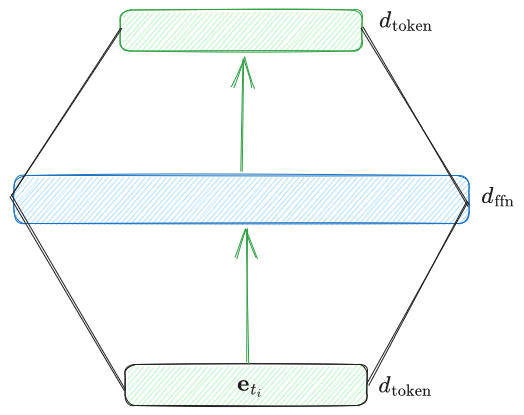
\includegraphics[width=1\textwidth]{assets/pics/ffn_transformer.png}
		\caption{Ilustrasi \f{position-wise feed-forward network} pada \f{transformer}.}
		\label{fig:position-wise-feed-forward-network}
	\end{figure}

	\f{Position-wise Feed-Foward Network} adalah \f{feed foward network} dengan dua kali transformasi linear dan sebuah fungsi aktivasi ReLU di antaranya. \pic~\ref{fig:position-wise-feed-forward-network} menunjukkan ilustrasi dari \f{position-wise feed-forward network} dan \equ~\ref{equ:position-wise-feed-forward-network-start} hingga \equ~\ref{equ:position-wise-feed-forward-network-end} menunjukkan Transformasi yang dilakukan oleh \f{position-wise feed-forward network}.

	\begin{align}
		\label{equ:position-wise-feed-forward-network-start}
		\text{FFN}(\mathbf{X}) &= \max(0, \mathbf{X}\mathbf{W}_1 + \mathbf{b}_1)\mathbf{W}_2 + \mathbf{b}_2 \in \mathbb{R}^{L \times d_{\text{token}}} \\
		\label{equ:position-wise-feed-forward-network-end}j
		\mathbf{W}_1 &\in \mathbb{R}^{d_{\text{token}} \times d_{\text{ffn}}}, \mathbf{W}_2 \in \mathbb{R}^{d_{\text{ffn}} \times d_{\text{token}}}, \mathbf{b}_1 \in \mathbb{R}^{d_{\text{ffn}}}, \mathbf{b}_2 \in \mathbb{R}^{d_{\text{token}}}.
	\end{align}

	$d_{\text{ffn}}$ adalah dimensi dari \f{feed forward network} yang digunakan. \cite{transformerori} menggunakan $d_{\text{ffn}} = 2048$.

	\subsection{Koneksi Residual dan \f{Layer Normalization}}
	\label{sec:layer-normalization}

	Pada tahap pelatihan, pembaruan parameter model dilakukan pada semua \f{layer} secara serentak setiap iterasi pelatihan. Ketika parameter suatu \f{layer} mengalami pembaharuan, distribusi dari \f{output} yang dihasilkan \f{layer} tersebut juga akan berubah pada iterasi selanjutnya. \f{Layer-layer} selanjutnya harus beradaptasi karena distribusi \f{input}-nya dari \f{layer} tersebut berubah. Fenomena ini disebut \f{internal covariate shift} yang mengakibatkan proses pencarian parameter menjadi lebih lambat.

	\f{Layer Normalization} berfungsi untuk mencegah masalah \f{internal covariate shift} di atas dengan membatasi distribusi nilai \f{output} yang nantinya menjadi \f{input} pada \f{layer} selanjutnya. Justifikasi lainnya di balik penggunaan \f{layer normalization} adalah variansi dari \f{input} dari \f{self-attention layer} haruslah 1, sehingga variansi dari bobot atensi $\text{Softmax}(\frac{\mathbf{EW}^q (\mathbf{EW}^k)^{\top}}{\sqrt{d_{\text{token}}}})$ akan 1 juga.

	\equ~\ref{equ:layer-normalization-start} hingga \equ~\ref{equ:layer-normalization-end} menunjukkan proses kerja dari \f{layer normalization}.

	\begin{align}
		\label{equ:layer-normalization-start}
		\mathbf{X} &= \begin{bmatrix}
		x_{11} & x_{12} & \dots & x_{1,d_{\text{token}}} \\
		x_{21} & x_{22} & \dots & x_{2,d_{\text{token}}} \\
		\vdots & \vdots & \ddots & \vdots \\
		x_{L1} & x_{L2} & \dots & x_{L,d_{\text{token}}} \\
		\end{bmatrix} \in \mathbb{R}^{L \times d_{\text{token}}} \\
		\text{LayerNorm}(\mathbf{X}) &= (\mathbf{X}-\bm{\mu})\odot \frac{1}{\bm{\sigma}}\\
		&= \begin{bmatrix}
		\frac{x_{11}-\mu_1}{\sigma_1} & \frac{x_{12}-\mu_1}{\sigma_1} & \dots & \frac{x_{1,d_{\text{token}}}-\mu_1}{\sigma_1} \\
		\frac{x_{21}-\mu_2}{\sigma_2} & \frac{x_{22}-\mu_2}{\sigma_2} & \dots & \frac{x_{2,d_{\text{token}}}-\mu_2}{\sigma_2} \\
		\vdots & \vdots & \ddots & \vdots \\
		\frac{x_{L1}-\mu_L}{\sigma_L} & \frac{x_{L2}-\mu_L}{\sigma_L} & \dots & \frac{x_{L,d_{\text{token}}}-\mu_L}{\sigma_L} \\
		\end{bmatrix} \in \mathbb{R}^{L \times d_{\text{token}}} \\
		\bm{\mu} &= \begin{bmatrix}
		\mu_1 &\dots & \mu_1 \\
		\vdots & \ddots &\vdots \\
		\mu_L & \dots & \mu_L
		\end{bmatrix} \in \mathbb{R}^{L\times d_{\text{token}}}, \\
		\frac{1}{\bm{\sigma}} &= \begin{bmatrix}
		\frac{1}{\sigma_1} &\dots & \frac{1}{\sigma_1} \\
		\vdots & \ddots &\vdots \\
		\frac{1}{\sigma_L} &\dots & \frac{1}{\sigma_L} \\
		\end{bmatrix} \in \mathbb{R}^{L\times d_{\text{token}}}, \\
		\mu_i &= \frac{1}{d_\text{token}}\sum_{j=1}^{d_{\text{token}}} x_{ij},\quad i=1,\dots,L, \\
		\sigma_i &= \sqrt{\frac{1}{d_{\text{token}}} \sum_{j=1}^{d_{\text{token}}} (x_{ij}-\mu_i)^2}, \quad i = 1,\dots, L, \\
		\label{equ:layer-normalization-end}
		\odot &= \text{element-wise product.} 
		\end{align}

	\subsection{Transformer Encoder}
	\label{sec:encoder}

	Dengan menggunakan \f{multi-head self-attention layer}, \f{position-wise feed-forward network layer}, dan \f{layer normalization} dan \f{residual connection} yang sudah dijelaskan sebelumnya, blok enkoder pada \f{transformer} enkoder dapat ditulis seperti pada \equ~\ref{equ:transformer-encoder-start} hingga \equ~\ref{equ:transformer-encoder-end}.

	\begin{align}
		
	\end{align}


\section{Bidirectional Encoder Representations from Transformers (BERT)}
	\subsection{Representasi Input}
	
	\subsection{Model Pralatih BERT}

		\subsubsection{\f{Masked Language Model}}

		\subsubsection{\f{Next Sentence Prediction}}

	\subsection{BERT untuk Bahasa Indonesia (IndoBERT)}

	\subsection{Penggunaan BERT untuk Pemeringkatan Teks}
		\subsubsection{$\text{BERT}_{\text{CAT}}$}

		\subsubsection{$\text{BERT}_{\text{DOT}}$}





\clearchapter
\chapter{\babEmpat}
\label{bab:4}

Bab ini membahas mengenai proses \f{fine tuning} model \f{Bidirectional Encoder Representations from Transformers} (BERT) untuk mendapatkan model yang dapat digunakan pada masalah pemeringkatan teks.
\sect~\ref{sec:spesifikasi} menjelaskan mengenai spesifikasi perangkat keras dan perangkat lunak yang digunakan dalam penelitian. Selanjutnya, \sect~\ref{sec:simulasi} menjelaskan mengenai tahapan simulasi yang dilakukan dalam penelitian. Informasi mengenai \f{dataset} latih dan uji  dijelaskan pada \sect~\ref{sec:dataset}. \sect~\ref{sec:finetuning} menjelaskan lebih detail mengenai arsitektur model BERT, fungsi loss, serta konfigurasi \f{hyperparameter} yang digunakan dalam proses \f{fine tuning} model BERT. Terakhir, \sect~\ref{sec:hasil} menjelaskan mengenai evaluasi hasil \f{fine tuning} model BERT untuk pemeringkatan teks.

\section{Spesifikasi Mesin dan Perangkat Lunak}
\label{sec:spesifikasi}

Proses \f{fine tuning} model BERT untuk pemeringkatan teks dilakukan menggunakan mesin dan perangkat lunak yang tertera pada \tab~\ref{tab:spesifikasi}.
\begin{table}[!ht]
    \centering
    \caption{Spesifikasi perangkat lunak yang digunakan pada penelitian ini.}
    \label{tab:spesifikasi}
    \begin{tabular}{|l|l|} \hline
        \textbf{CPU}                         & AMD Ryzen 9 5950X 32-Core Processor                                                                                                      \\ \hline
        \textbf{GPU}                         & NVIDIA GeForce RTX 4090 24GB                                                                                                             \\ \hline
        \textbf{Memori}                      & 64GB                                                                                                                                     \\ \hline
        \textbf{Sistem Operasi}              & Ubuntu 20.04.2 LTS                                                                                                                       \\ \hline
        \textbf{Perangkat Lunak Pemrograman} & Visual Studio Code 1.84.2                                                                                                                \\ \hline
        \textbf{Bahasa Pemrograman}          & Python 3.8                                                                                                                               \\ \hline
        \textbf{Pustaka yang Digunakan}      & \begin{tabular}[c]{@{}l@{}}sentence-transformers 2.2.2\\ transformers 4.35.1\\ beir 2.0.0\\ gdown 4.7.1\\ torch 2.0.1+cu117\end{tabular} \\ \hline
    \end{tabular}
\end{table}

\section{Tahapan Simulasi}
\label{sec:simulasi}

\pic~\ref{fig:diagram-simulasi} menunjukkan tahapan simulasi yang dilakukan dalam penelitian ini.
\begin{figure}
    \centering
    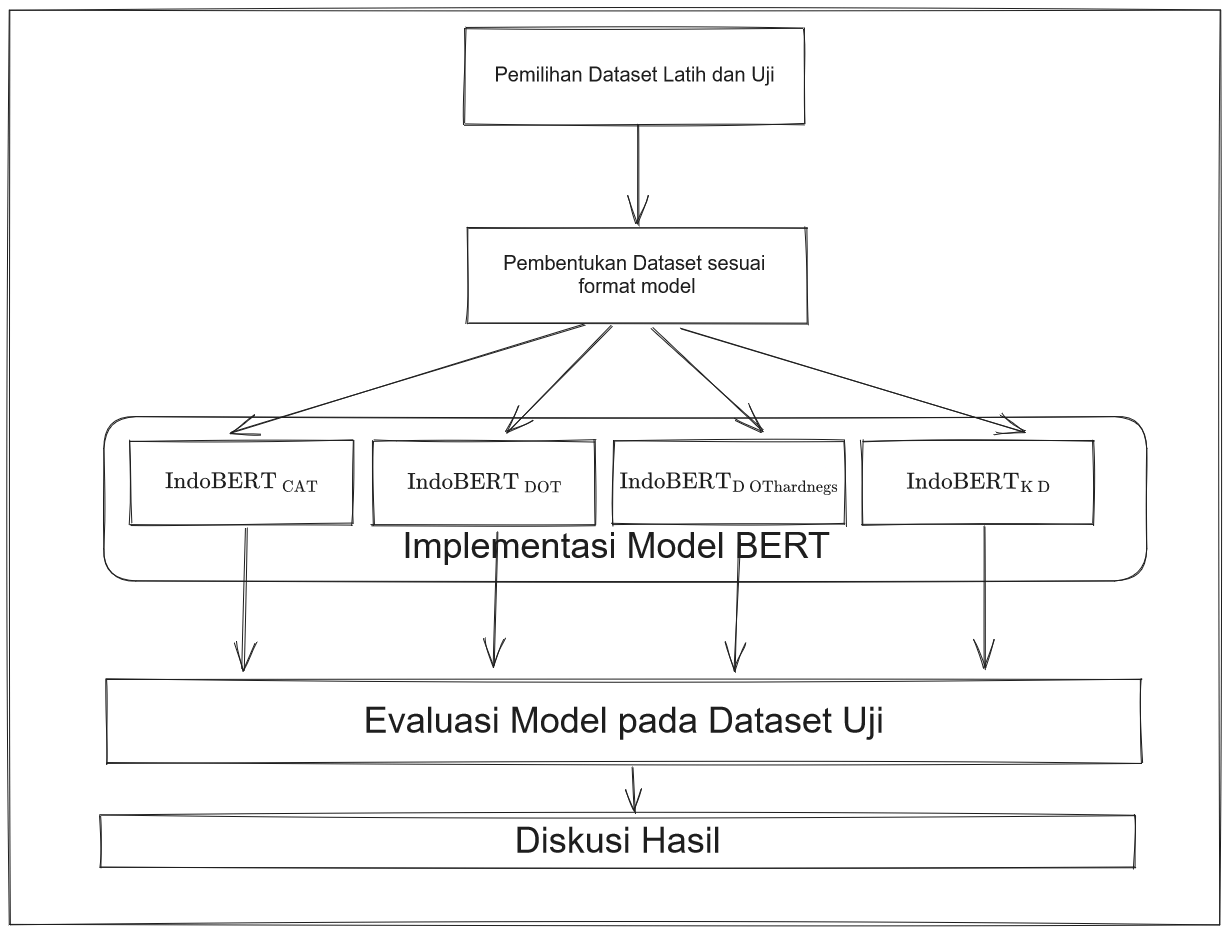
\includegraphics[width=1\textwidth]{assets/pics/alursimulasi.png}
    \caption{Diagram Simulasi}
    \label{fig:diagram-simulasi}

\end{figure}

Simulasi diawali dengan pengambilan data. Data yang digunakan adalah data pada penelitian \cite{mmarco}, sebagai \f{dataset} latih, dan data pada penelitian \cite{mrtydi}, \cite{miracl} sebagai \f{dataset} uji. \f{Dataset} latih tidak dapat digunakan langsung untuk melatih model-model tersebut. Untuk setiap modelnya, diperlukan transformasi untuk mengubah bentuk dari \f{dataset} latih sehingga sesuai dengan formatnya. Transformasi \f{dataset} latih dan \f{hyperparameter} dari model akan dibahas lebih lanjut pada bagian \sect~\ref{sec:finetuning}. Selanjutnya, proses implementasi dan pelatihan model dilakukan. Setelah itu, akan dilakukan evaluasi setiap model pada \f{dataset} uji. Terdapat satu model BM25 sebagai \f{baseline} untuk membandingkan hasil evaluasi dari model-model yang dilatih. Terakhir, terdapat diskusi mengenai hasil evaluasi tersebut.

\section{Data}
\label{sec:dataset}

Penelitian ini menggunakan satu \f{dataset} latih mMarco \f{train set} bahasa Indonesia \citep{mmarco} dan tiga \f{dataset} uji, yaitu mMarco \f{dev set} bahasa Indonesia, MrTyDi Test set Indonesia \citep{mrtydi}, dan Miracl \f{dev set} bahasa Indonesia \citep{miracl}. \f{Dataset} Miracl dan MrTyDi dipilih sebagai uji kemampuan \f{out-of-distibution} dari model yang dihasilkan. Setiap \f{dataset} terdiri dari 3 \f{file}, yaitu \f{file} kueri, \f{file} korpus dan \f{file jugdements} yang telah dijelaskan pada \sect~\ref{sec:dataset-umum}. \tab~\ref{tab:dataset-info} menunjukkan informasi mengenai jumlah entri dari \f{file} kueri, \f{file korpus}, dan \f{file jugdements} dari setiap \f{dataset} yang digunakan dalam penelitian ini.
\begin{table}
    \centering
    \captionsource{Tabel Informasi untuk Setiap \f{Dataset}. Kolom \f{Korpus} menunjukkan jumlah entri pada \f{file korpus}, kolom \f{Kueri} menunjukkan jumlah entri pada \f{file kueri}, dan kolom \f{Jugdements} menunjukkan jumlah entri pada \f{file jugdements} (pasangan kueri dan teks dengan nilai relevansi).}{\citep{attentionkernel}}
    \label{tab:dataset-info}
    \begin{tabular}{|l|c|c|c|} \hline
        \textbf{Dataset} & \textbf{Korpus} & \textbf{Kueri} & \textbf{Jugdements} \\ \hline
        mMarco train set & 8,841,823       & 1,010,916      & 532,761             \\ \hline
        mMarco dev set   & 8,841,823       & 1,010,916      & 7,437               \\ \hline
        Mrtydi test set  & 1,469,399       & 829            & 961                 \\ \hline
        Miracl dev set   & 1,446,315       & 960            & 9,668               \\ \hline
    \end{tabular}
\end{table}

Setiap \f{judgements} pada \f{dataset} adalah \f{jugdgements} biner, yaitu bernilai 1 jika teks tersebut relevan dengan kueri dan 0 jika tidak relevan dengan kueri. \tab~\ref{tab:contoh-file-korpus-bab4} hingga \tab~\ref{tab:judgements-file-example-bab4} menunjukkan contoh dari \f{file} korpus, \f{file} kueri, dan \f{file jugdements} pada \f{dataset} Miracl \f{dev set}.
\begin{table}
    \centering
    \caption{Potongan \f{file} korpus \f{dataset} Miracl.}
    \label{tab:contoh-file-korpus-bab4}
    \begin{tabular}{|l|l|p{0.6\textwidth}|}
        \hline
        \textbf{\_id}    & \textbf{title}             & \textbf{text}                                                                                                 \\ \hline
        1342516\#1  & Colobothea biguttata & Larva kumbang ini biasanya mengebor ke dalam kayu dan dapat menyebabkan kerusakan pada batang kayu hidup atau kayu yang telah ditebang. \\ \hline
        1342517\#0  & Ichthyodes rufipes  & Ichthyodes rufipes adalah spesies kumbang tanduk panjang yang berasal dari famili Cerambycidae. Spesies ini juga merupakan bagian dari genus Ichthyodes, ordo Coleoptera, kelas Insecta, filum Arthropoda, dan kingdom Animalia. \\ \hline
    \end{tabular}
\end{table}

\begin{table}
    \centering
    \caption{Potongan \f{file} kueri \f{dataset} Miracl.}
    \label{tab:query-file-example-bab4}
    \begin{tabular}{|l|p{0.8\textwidth}|}
        \hline
        \textbf{\_id} & \textbf{text}                                                                 \\ \hline
        3             & Dimana James Hepburn meninggal?                                              \\ \hline
        4             & Dimana Jamie Richard Vardy lahir?                                            \\ \hline
        11            & berapakah luas pulau Flores?                                                 \\ \hline
        17            & Siapakah yang menulis Candy Candy?                                           \\ \hline
        19            & Apakah karya tulis Irma Hardisurya yang pertama?                              \\ \hline
    \end{tabular}
\end{table}

\begin{table}
    \centering
    \caption{Potongan \f{file} judgements \f{dataset} Miracl.}
    \label{tab:judgements-file-example-bab4}
    \begin{tabular}{|l|l|l|}
        \hline
        \textbf{query-id} & \textbf{corpus-id} & \textbf{score} \\ \hline
        3                 & 115796\#6          & 1              \\ \hline
        3                 & 77689\#48          & 1              \\ \hline
        4                 & 1852373\#0         & 1              \\ \hline
    \end{tabular}
\end{table}


\section{\f{Fine Tuning} Model BERT}
\label{sec:finetuning}

Bagian ini menjelaskan mengenai konfigurasi \f{hyperparameter} yang digunakan pada setiap model yang dikerjakan pada peneletian ini. Terdapat empat model yang dikerjakan pada penelitian ini, yaitu $\text{IndoBERT}_{\text{CAT}}$, $\text{IndoBERT}_{\text{DOT}}$, $\text{IndoBERT}_{\text{DOThardnegs}}$, dan $\text{IndoBERT}_{\text{DOTKD}}$. Keempat model tersebut merupakan model BERT yang dilatih dengan menggunakan \f{dataset} mMarco \f{train set} dengan prosedur yang berbeda-beda.

\subsection{$\text{IndoBERT}_{\text{CAT}}$}

Pada model $\text{IndoBERT}_{\text{CAT}}$, arsitektur $\text{BERT}_\text{CAT}$ (lihat \sect~\ref{sec:bert-cat}) digunakan untuk melakukan pemeringkatan teks. Proses pelatihan model menggunakan \f{dataset} yang digunakan berasal dari mMarco \f{train set} dengan format $(q, d, r)$ dengan $q$ adalah kueri, $d$ adalah teks, dan $r$ adalah relevansi teks $d$ terhadap kueri $q$. Pelatihan yang dilakukan seperti melakukan klasifikasi relevansi teks terhadap kueri. Perlu dicatat bahwa tidak ada contoh $r=0$ dalam \f{dataset} mMarco \f{train set} (lihat \sect~\ref{sec:dataset-umum}).

Untuk membentuk data latih dengan penilaian $r=0$, pasangan $(q, d',0)$ ditambahkan dengan $d'$ sebagai teks acak yang tidak relevan dengan kueri $q$. \f{Dataset} yang telah dibuat terdiri dari 500 ribu pasangan $(q, d, r)$ dengan rasio 1:1 antara $r=1$ dan $r=0$. Potongan \f{dataset} yang digunakan untuk pelatihan model $\text{IndoBERT}_{\text{CAT}}$ dapat ditemukan pada \tab~\ref{tab:contoh-indobert-cat-data}.
\begin{table}
    \centering
    \caption{Potongan \f{dataset} yang digunakan untuk pelatihan model $\text{IndoBERT}_{\text{CAT}}$.}
    \label{tab:contoh-indobert-cat-data}
    \begin{tabular}{|p{2cm}|p{7cm}|c|} \hline
        \textbf{Kueri}                                         & \textbf{Teks}                                                                                                                                                                                                                                                                                                                                                                                                                                                                                                                                                                                          & \textbf{Relevansi} \\ \hline
        Berapa banyak kalori sehari yang hilang saat menyusui? & Tidak hanya menyusui lebih baik untuk bayi, namun penelitian juga mengatakan itu lebih baik bagi ibu. Menyusui membakar rata-rata 500 kalori sehari, dengan kisaran khas antara 200 hingga 600 kalori yang terbakar sehari. Diperkirakan produksi 1 oz. ASI membakar 20 kalori. Jumlah kalori yang terbakar tergantung pada seberapa banyak bayi makan. Menyusui kembar membakar dua kali lebih banyak daripada memberi makan hanya satu bayi. Dengan anak kembar, ibu mereka membakar 1000 kalori per hari. Membakar 500 kalori ekstra sehari akan menghasilkan satu pon penurunan berat badan mingguan. & 1                  \\ \hline
        Karakteristik iklim utama hutan hujan tropis           & Kacang kola adalah buah dari pohon kola, genus (Cola) pohon yang berasal dari hutan hujan tropis Afrika. & 0                  \\ \hline
    \end{tabular}
\end{table}

Konfigurasi \f{hyperparameter} selama pelatiahan model $\text{indoBERT}_{\text{CAT}}$ dapat  dilihat pada \tab~\ref{tab:indobert-cat-hyperparameter}.

\begin{table}
    \centering
    \caption{\f{Hyperparameter} yang digunakan untuk \f{fine tuning }$\text{IndoBERT}_{\text{CAT}}$.}
    \label{tab:indobert-cat-hyperparameter}
    \begin{tabular}{|c|c|}
        \hline
        \textbf{Parameter}       & \textbf{Nilai}                                                                                    \\
        \hline
        Model pralatih           & \href{https://huggingface.co/indolem/indobert-base-uncased}{\code{indolem/indobert-base-uncased}} \\
        \hline
        Total data               & 500,000                                                                                     \\
        \hline
        \f{Batch size}           & 32                                                                                                \\
        \hline
        Total iterasi            & 78125 (5 epochs)                                                                                  \\
        \hline
        \f{Optimizer}            & Adam dengan $\beta_1 = 0.9$, $\beta_2 = 0.999$, $\epsilon = 1e-8$                                 \\
        \hline
        \f{Learning rate}        & 2e-5                                                                                              \\
        \hline
        \f{Learning rate warmup} & Linear selama 10\% dari total iterasi                                                             \\
        \hline
        Fungsi loss              & \f{Binary cross entropy}                                                                          \\
        \hline
    \end{tabular}
\end{table}

\subsection{$\text{IndoBERT}_{\text{DOT}}$}
Pada model $\text{IndoBERT}_{\text{DOT}}$, arsitektur $\text{BERT}_\text{DOT}$ (lihat \sect~\ref{sec:bert-dot}) digunakan untuk melakukan pemeringkatan teks. fungsi loss yang digunakan untuk pelatihan model $\text{IndoBERT}_{\text{DOT}}$ adalah \f{N-pair loss}. Untuk kueri $q$, teks relevan $d^+$, dan kumpulan teks tidak relevan $\{d_i^-\}_{i=1}^{N-1}$ terhadap kueri $q$, \f{N-pair loss} dihitung sebagai berikut:
\begin{align}
    L(q, d^+,\{d_i^-\}_{i=1}^{N-1}) = -\log \frac{\exp(\mathbf{h}^{\top}_q \mathbf{h}^+_d)}{\exp(\mathbf{h}^{\top}_q \mathbf{h}^+_d) + \sum_{i=1}^{N-1} \exp(\mathbf{h}^{\top}_q \mathbf{h}^-_i)},
\end{align}
dengan keterangan sebagai berikut:
\begin{flalign*}
    \mathbf{h}_q   &= \text{IndoBERT}_{\text{DOT}}((\text{[CLS]}, q, \text{[SEP]}))_{\text{[CLS]}} &&   \\
    \mathbf{h}^+_d &= \text{IndoBERT}_{\text{DOT}}((\text{[CLS]}, d^+, \text{[SEP]}))_{\text{[CLS]}} && \\
    \mathbf{h}^-_i &= \text{IndoBERT}_{\text{DOT}}((\text{[CLS]}, d^-_i, \text{[SEP]}))_{\text{[CLS]}} && \\
\end{flalign*}

Pasangan $(q,d^+)$ diambil langsung dari \f{file judgements} pada mMarco \f{train set}. Kumpulan teks tak relevan $\{d_i^-\}_{i=1}^{N-1}$ dibentuk dengan menggunakan teks $d$ pada \f{data point} yang berbeda pada \f{batch} yang sama. Nilai $N$ pada \f{N-pair loss} adalah ukuran \f{batch} yang digunakan selama pelatihan model. Metode pemilihan teks negatif ini disebut dengan \f{in-batch negative sampling} \citep{dprmeta}. Pada penelitian ini, digunakan seluruh \f{datapoint} pada \f{file jugdements} mMarco \f{train set} -- 532,761 \f{data point} -- untuk membentuk \f{dataset} latih model $\text{IndoBERT}_{\text{DOT}}$.

Konfigurasi \f{hyperparameter} selama pelatiahan model $\text{indoBERT}_{\text{DOT}}$ dapat  dilihat pada \tab~\ref{tab:indobert-dot-hyperparameter}.
\begin{table}[!ht]
    \centering
    \caption{\f{Hyperparameter} yang digunakan untuk \f{fine tuning }$\text{IndoBERT}_{\text{DOT}}$.}
    \label{tab:indobert-dot-hyperparameter}
    \begin{tabular}{|c|c|}
        \hline
        \textbf{Parameter}       & \textbf{Nilai}                                                                                    \\
        \hline
        Model pralatih           & \href{https://huggingface.co/indolem/indobert-base-uncased}{\code{indolem/indobert-base-uncased}} \\
        \hline
        Total data               & 532,761                                                                                           \\
        \hline
        \f{Batch size}           & 32                                                                                                \\
        \hline
        Total iterasi            & 83243 (5 epochs)                                                                                  \\
        \hline
        \f{Optimizer}            & Adam dengan $\beta_1 = 0.9$, $\beta_2 = 0.999$, $\epsilon = 1e-8$                                 \\
        \hline
        \f{Learning rate}        & 2e-5                                                                                              \\
        \hline
        \f{Learning rate warmup} & Linear selama 10\% dari total iterasi                                                             \\
        \hline
        Fungsi \f{loss}          & \f{N-pair loss}                                                                                   \\
        \hline
    \end{tabular}
\end{table}

\subsection{$\text{IndoBERT}_{\text{DOThardnegs}}$}

Pada $\text{IndoBERT}_\text{DOThardnegs}$, arsitektur $\text{BERT}_\text{DOT}$ digunakan untuk melakukan pemeringkatan teks. Fungsi loss yang digunakan untuk pelatihan model $\text{IndoBERT}_{\text{DOThardnegs}}$ adalah \f{N-pair loss} seperti $\text{IndoBERT}_{\text{DOT}}$. Perbedaan utama antara $\text{IndoBERT}_{\text{DOT}}$ dan $\text{IndoBERT}_{\text{DOThardnegs}}$ pada metode pemilihan teks negatif. Pada $\text{IndoBERT}_{\text{DOThardnegs}}$, teks negatif sudah terlebih dahulu dipilih dengan kriteria bahwa teks tersebut adalah teks yang tidak relevan dengan kueri $q$, tetapi pemeringkatan dengan BM25 berada di 100 teratas. Dengan kata lain, teks negatif adalah teks yang sulit dibedakan dengan teks positif ketika menggunakan BM25. Teks \f{hard negative} ini diberikan oleh suatu \f{file} dan \tab~\ref{tab:hardnegsbm25} menunjukkan contoh dari teks \f{file} tersebut. Nilai $N$ yang dipilih pada penelitian ini adalah $N=5$, dan jumlah data yang digunakan adalah 502.939 \f{data point}.

\begin{table}[!ht]
    \centering
    \captionsource{Potongan \f{file hard negative}. Kolom qid berisikan id dari kueri, kolom \f{positive} adalah id teks positif, dan kolom \f{hard negative} adalah id teks yang sulit dibedakan dengan teks positif menggunakan BM25.}{\url{https://huggingface.co/datasets/carles-undergrad-thesis/mmarco-hardnegs-bm25}}
    \label{tab:hardnegsbm25}
    \begin{tabular}{|c|c|p{8cm}|}
        \hline
        qid & \f{Positive} & \f{Hard Negative}                                           \\
        \hline
        1185869 &  0  & [ 2942572, 5154062, 2942571, 5154065, 3870084 ] \\
        \hline
        1185868 &  16  & [ 6821177, 1641650, 1641656, 1641659, 1203539 ] \\
        \hline
        597651 &  49  & [ 6398884, 162755, 1838949, 1391482, 7818305 ] \\
        \hline
    \end{tabular}
\end{table}


Konfigurasi \f{hyperparameter} selama pelatiahan model $\text{indoBERT}_{\text{DOThardnegs}}$ dapat  dilihat pada \tab~\ref{tab:indobert-dothardnegs-hyperparameter}.

\begin{table}[!ht]
    \centering
    \caption{\f{Hyperparameter} yang digunakan untuk \f{fine tuning }$\text{IndoBERT}_{\text{DOThardnegs}}$.}
    \label{tab:indobert-dothardnegs-hyperparameter}
    \begin{tabular}{|c|c|}
        \hline
        \textbf{Parameter}       & \textbf{Nilai}                                                                                    \\
        \hline
        Model pralatih           & \href{https://huggingface.co/indolem/indobert-base-uncased}{\code{indolem/indobert-base-uncased}} \\
        \hline
        Total data               & 502,939                                                                                           \\
        \hline
        \f{Batch Size}           & 32                                                                                                \\
        \hline
        Total Iterasi            & 78585 (5 epochs)                                                                                  \\
        \hline
        \f{Optimizer}            & Adam dengan $\beta_1 = 0.9$, $\beta_2 = 0.999$, $\epsilon = 1e-8$                                 \\
        \hline
        \f{Learning rate}        & 2e-5                                                                                              \\
        \hline
        \f{Learning rate warmup} & Linear selama 10\% dari total iterasi                                                             \\
        \hline
        Fungsi \f{loss}          & \f{N-pair loss}                                                                                   \\
        \hline
    \end{tabular}
\end{table}


\subsection{$\text{IndoBERT}_{\text{DOTKD}}$}
$\text{IndoBERT}_{\text{DOTKD}}$ dilatih dengan menggunakan prinsip \f{knowledge distillation}, yaitu proses \f{transfer} pengetahuan dari model yang sudah dilatih dengan baik (guru) ke model yang belum dilatih (murid). Model yang digunakan sebagai guru adalah model bahasa Inggris yang sudah dilatih dengan baik untuk melakukan pemeringkatan teks. Model Murid yang dapat dipilih adalah model pralatih BERT multibahasa -- model yang \f{pre-training}-nya dilakukan pada korpus multibahasa seperti mBERT (\f{mulitingual} BERT). Pemetaaan vektor dari model murid akan di-\f{align} dengan Pemetaan vektor dari model guru dengan fungsi \f{loss} berikut:
\begin{align}
    L(s_i, t_i) = \left((\mid \mid M(s_i) - \hat{M}(s_i) \mid \mid)^2 + (\mid\mid M(s_i) - \hat{M}(t_i) \mid\mid)^2 \right),
\end{align}
dengan keterangan sebagai berikut:
\begin{flalign*}
    M        &= \text{pemeataan vektor oleh model guru},&& \\
    \hat{M}  &= \text{pemetaan vektor oleh model murid},&& \\
    s_i      &= \text{teks sumber (bahasa Inggris)},&& \\
    t_i      &= \text{teks target (bahasa Indonesia)}.&&
\end{flalign*}
\pic~\ref{fig:kd} menunjukkan ilustrasi dari proses pelatihan dengan \f{knowledge distillation}. 500 ribu kueri dan 500 ribu korpus dari mMarco \f{train set} Indonesia di-\f{align} dengan terjemahannya seperti yang ditunjukkan pada \tab~\ref{tab:sentence-parallel}.
\begin{figure}
    \centering
    \includegraphics[width=1\textwidth]{assets/pics/kd.png}
    \captionsource{Ilustrasi dari pelatihan model $\text{IndoBERT}_{\text{DOTKD}}$ dengan \f{knowledge distillation}. Kalimat paralel diberikan sebagai \f{input}  pada model guru dan model murid. vektor yang dihasilkan oleh model guru dan model murid di-\f{align} menggunakan fungsi \f{loss mean squared error}.}{\citep{knowledgedistill}} 
    \label{fig:kd}
\end{figure}
\begin{table}
    \centering
    \captionsource{Potongan dari \f{dataset} yang digunakan untuk pelatihan model $\text{IndoBERT}_{\text{KD}}$.}{\href{https://huggingface.co/datasets/carles-undergrad-thesis/en-id-parallel-sentences}{\code{carles-undergrad-thesis/en-id-parallel-sentences}}}
    \label{tab:sentence-parallel}
    \begin{tabular}{|p{5cm}|p{5cm}|}
        \hline
        \textbf{text\_en} & \textbf{txt\_id} \\
        \hline
        \f{Defining alcoholism as a disease is associated with Jellinek} & Mendefinisikan alkoholisme sebagai penyakit dikaitkan dengan Jellinek \\
        \hline
        \f{ECT is a treatment that is used for} & ECT adalah pengobatan yang digunakan untuk \\
        \hline
        \f{Ebolavirus is an enveloped virus, which means} & Ebolavirus adalah virus yang diselimuti, yang berarti \\
        \hline
        \f{How much does Cambridge Manor cost per month} & Berapa biaya Cambridge Manor per bulan? \\
        \hline
    \end{tabular}
\end{table}

Konfigurasi \f{hyperparameter} selama pelatiahan model $\text{indoBERT}_{\text{KD}}$ dapat  dilihat pada \tab~\ref{tab:indobert-kd-hyperparameter}.

\begin{table}
    \centering
    \caption{ \f{Hyperparameter} yang digunakan untuk \f{fine tuning }$\text{IndoBERT}_{\text{DOTKD}}$.}
    \label{tab:indobert-kd-hyperparameter}
    \begin{tabular}{|c|c|}
        \hline
        \textbf{Parameter}       & \textbf{Nilai}                                                                                    \\
        \hline
        Model guru              & \href{https://huggingface.co/sentence-transformers/msmarco-bert-base-dot-v5}{\code{sentence-transformers/msmarco-bert-base-dot-v5}} \\
        \hline
        Model murid           & \href{https://huggingface.co/bert-base-multilingual-uncased}{\code{bert-base-multilingual-uncased}} \\
        \hline
        Total data               & 1,000,000                                                                                           \\
        \hline
        \f{Batch Size}           & 64                                                                                                \\
        \hline
        Total Iterasi            & 78125 (5 epochs)                                                                                  \\
        \hline
        \f{Optimizer}            & Adam dengan $\beta_1 = 0.9$, $\beta_2 = 0.999$, $\epsilon = 1e-8$                                 \\
        \hline
        \f{Learning rate}        & 2e-5                                                                                              \\
        \hline
        \f{Learning rate warmup} & Linear selama 10\% dari total iterasi                                                             \\
        \hline
        Fungsi \f{loss}          & \f{Mean squared error}                                                                            \\
        \hline
    \end{tabular}
\end{table}



\section{Evaluasi Model}
\label{sec:hasil}

Subbab ini membahas perihal hasil dari \f{Fine tuning} dan evaluasi dari keempat model. BM25 digunakan sebagai \f{baseline} untuk membandingkan evaluasi setiap model. BM25 yang digunakan adalah \f{software} \f{Elastic search} (\url{https://www.elastic.co/elasticsearch/}) untuk bahasa Indonesia dengan konfigurasi parameter \f{default}. 

Metrik yang digunakan pada \f{datasets} mMarco \f{dev set} dan MrTyDi \f{test set} adalah \f{Reciprocal Rank} pada 10 teks teratas (RR@10) dan \f{Recall} pada 1000 teks teratas (R@1000). Berbeda dengan mMarco dan MrTyDi,  Metrik yang digunakan pada \f{dataset} Miracl \f{dev set} adalah \f{Normalized Discounted Cumulative Gain} pada 10 teks teratas (NDCG@10) dan \f{Recall} pada 1000 teks teratas (R@1000). Perhitungan metrik lainnya untuk setiap model dapat dilihat pada bagian lampiran.

\subsection{Evaluasi $\text{IndoBERT}_{\text{CAT}}$}
\label{sec:resultindobertcat}

\begin{table}
    \centering
    \caption{Evaluasi model $\text{IndoBERT}_{\text{CAT}}$ pada \f{dataset} mMarco \f{dev set}, MrTyDi \f{test set}, dan Miracl \f{dev set}.}
    \label{tab:indobertcat-hasil}
    \begin{tabular}{|c|c|c|c|c|c|c|} \hline
        Model                             & \multicolumn{2}{c|}{mMarco Dev} &
        \multicolumn{2}{c|}{MrTyDi Test} & \multicolumn{2}{c|}{Miracl Dev}                                             \\ \hline
                                          & RR@10 & R@1000 & RR@10 & R@1000 & NDCG@10 & R@1000 \\ \hline
        BM25                              & .114  & \bo{.642}   & .279   & \bo{.858}   & .391    & \bo{.971} \\ \hline
        BM25+$\text{IndoBERT}_{\text{CAT}}$    & \bo{.181}  & \bo{.642}   & \bo{.447}   & \bo{.858}   & .\bo{455}    & \bo{.971} \\ \hline
    \end{tabular}
\end{table}


\tab~\ref{tab:indobertcat-hasil} menujukkan evaluasi dan perbandingan antara model $\text{IndoBERT}_{\text{CAT}}$ dan BM25. Perlu diingat kembali bahwa model $\text{IndoBERT}_{\text{CAT}}$ digunakan sebagai \f{reranker} (lihat \sect~\ref{sec:bert-cat}) untuk memperbaiki hasil dari BM25. Efeknya nilai \f{Recall} dari model $\text{IndoBERT}_{\text{CAT}}$ sama dengan nilai \f{Recall} dari BM25. Namun, nilai \f{Reciprocal Rank} dari model $\text{IndoBERT}_{\text{CAT}}$ lebih tinggi dari BM25. Hal ini menunjukkan bahwa model $\text{IndoBERT}_{\text{CAT}}$ lebih baik dalam memberikan urutan teks yang direkomendasikan oleh BM25.

nilai RR@10 dari model $\text{IndoBERT}_{\text{CAT}}$ pada dataset mMarco \f{dev set} meningkat sebesar .67 poin (58\%) dibandingkan dengan BM25. Peningkatan yang sama juga terjadi pada nilai RR@10 MrTyDi \f{test set} dan nilai NDCG@10 Miracl \f{dev set} dengan peningkatan sebesar .168 poin (60\%) dan .064 poin (16\%) masing-masingnya.


\subsection{Evaluasi $\text{IndoBERT}_{\text{DOT}}$}
\label{sec:resultindobertdot}


\begin{table}
    \centering
    \caption{Evaluasi model $\text{IndoBERT}_{\text{DOT}}$ pada \f{dataset} mMarco \f{dev set}, MrTyDi \f{test set}, dan Miracl \f{dev set}.}
    
    \label{tab:indobertdot-hasil}
    \begin{tabular}
        {|c|c|c|c|c|c|c|} \hline
        Model                             & \multicolumn{2}{c|}{mMarco Dev} &
        \multicolumn{2}{c|}{MrTyDi Test} & \multicolumn{2}{c|}{Miracl Dev}                                             \\ \hline
                                          & RR@10 & R@1000 & RR@10 & R@1000 & NCDG@10 & R@1000 \\ \hline
        BM25                              & .114  & .642   & .279   & .858   & \bo{.391}    & \bo{.971} \\ \hline
        $\text{IndoBERT}_{\text{DOT}}$    & \bo{.192}  & \bo{.847}   & \bo{.378}   & \bo{.936}   & .355    & .920 \\ \hline
        
    

    \end{tabular}

\end{table}

\tab~\ref{tab:indobertdot-hasil} menunjukkan evaluasi dan perbandingan antara model $\text{IndoBERT}_{\text{DOT}}$ dan BM25. Peningkatan terjadi pada nilai RR@10 dan R@1000 pada \f{dataset} mMarco \f{dev set} dan MrTyDi \f{test set}. Nilai RR@10 pada mMarco \f{dev set} meningkat sebesar .078 poin (68\%) dan pada MrTyDi \f{test set} sebesar .099 poin (35\%). Nilai R@1000 pada mMarco \f{dev set} meningkat sebesar .205 poin (32\%) dan pada MrTyDi \f{test set} sebesar .078 poin (9\%). Sementara itu, nilai NDCG@10 pada Miracl \f{dev set} menurun sebesar .036 poin (-9\%) dan nilai R@1000 juga menurun sebesar .051 poin (-5\%).

\subsection{Evaluasi $\text{IndoBERT}_{\text{DOThardnegs}}$}
\label{sec:resultindobertdothardnegs}

\begin{table}
    \centering
    \caption{Evaluasi model $\text{IndoBERT}_{\text{DOThardnegs}}$ pada \f{dataset} mMarco \f{dev set}, MrTyDi \f{test set}, dan Miracl \f{dev set}.}
    \label{tab:indobertdothardnegs-hasil}
    \begin{tabular}{|c|c|c|c|c|c|c|} \hline
        Model                                     & \multicolumn{2}{c|}{mMarco Dev} &
        \multicolumn{2}{c|}{MrTyDi Test}          & \multicolumn{2}{c|}{Miracl Dev}                                             \\ \hline
                                                  & RR@10 & R@1000 & RR@10 & R@1000 & NCDG@10 & R@1000 \\ \hline
        BM25                                      & .114  & .642   & .279   & .858   & .391    & \bo{.971} \\ \hline
        $\text{IndoBERT}_{\text{DOThardnegs}}$    & \bo{.232}  & \bo{.847}   & \bo{.471}   & \bo{.921}   & \bo{.397}    & .898 \\ \hline
    \end{tabular}
\end{table}

\tab~\ref{tab:indobertdothardnegs-hasil} menunjukkan evaluasi dan perbandingan antara model $\text{IndoBERT}_{\text{DOThardnegs}}$ dan BM25. Peningkatan terjadi pada nilai RR@10 dan R@1000 pada \f{dataset} mMarco \f{dev set} dan MrTyDi \f{test set}. Nilai RR@10 pada mMarco \f{dev set} meningkat sebesar .118 poin (103\%) dan pada MrTyDi \f{test set} sebesar .192 poin (69\%). Nilai R@1000 pada mMarco \f{dev set} juga meningkat sebesar .205 poin (32\%) dan pada MrTyDi \f{test set} sebesar .063 poin (7\%). Sementara itu, nilai NDCG@10 pada Miracl \f{dev set} menurun sebesar .006 poin (-1\%) dan nilai R@1000 juga menurun sebesar .073 poin (-8\%).


\subsection{Evaluasi $\text{IndoBERT}_{\text{KD}}$}
\label{sec:resultindobertkd}

\begin{table}
    \centering
    \caption{Evaluasi model $\text{IndoBERT}_{\text{KD}}$ pada \f{dataset} mMarco \f{dev set}, MrTyDi \f{test set}, dan Miracl \f{dev set}.}
    \label{tab:indobertkd-hasil}
    \begin{tabular}{|c|c|c|c|c|c|c|} \hline
        Model                             & \multicolumn{2}{c|}{mMarco Dev} &
        \multicolumn{2}{c|}{MrTyDi Test} & \multicolumn{2}{c|}{Miracl Dev}                                             \\ \hline
                                          & RR@10 & R@1000 & RR@10 & R@1000 & NCDG@10 & R@1000 \\ \hline
        BM25                              & .114  & .642   & .279   & .858   & \bo{.391}    & \bo{.971} \\ \hline
        $\text{IndoBERT}_{\text{DOTKD}}$  & \bo{.235}  & \bo{.867}   & \bo{.393}   & \bo{.882}   & .374    & .871    \\ \hline
    \end{tabular}
\end{table}

\tab~\ref{tab:indobertkd-hasil} menunjukkan evaluasi dan perbandingan antara model $\text{IndoBERT}_{\text{DOTKD}}$ dengan BM25. Peningkatan Terjadi pada nilai RR@10 dan R@1000 pada \f{dataset} mMarco \f{dev set}  dan MrTyDi \f{test set}. Nilai RR@10 pada mMarco \f{dev set} meningkat sebesar .121 poin (106\%) dan pada MrTyDi \f{test set} sebesar .114 poin (41\%). Nilai R@1000 pada mMarco \f{dev set} juga meningkat sebesar .225 poin (37\%) dan pada MrTyDi \f{test set} sebesar .024 poin (3\%). Sementara itu, nilai NDCG@10 pada Miracl \f{dev set} menurun sebesar .017 poin (-4\%) dan nilai R@1000 juga menurun sebesar .100 poin (-10\%).


\section{Diskusi Hasil}
\label{sec:diskusihasil}
\begin{table}
    \centering
    \caption{Evaluasi dari model $\text{IndoBERT}_{\text{CAT}}$, $\text{IndoBERT}_{\text{DOT}}$, $\text{IndoBERT}_{\text{DOThardnegs}}$, dan $\text{IndoBERT}_{\text{DOTKD}}$ pada \f{dataset} mMarco \f{dev set}, MrTyDi \f{test set}, dan Miracl \f{dev set}.}
    \label{tab:evaluasisemuamodel}
    \begin{tabular}{|c|c|c|c|c|c|c|} \hline
        Model                             & \multicolumn{2}{c|}{mMarco Dev} &
        \multicolumn{2}{c|}{MrTyDi Test} & \multicolumn{2}{c|}{Miracl Dev}                                             \\ \hline
                                          & RR@10 & R@1000 & RR@10 & R@1000 & NCDG@10 & R@1000 \\ \hline
        BM25                              & .114  & .642   & .279   & .858   & .391    & \bo{.971} \\ \hline
        BM25+$\text{IndoBERT}_{\text{CAT}}$    & .181  & .642   & .447   & .858   & \bo{.455}    & \bo{.971} \\ \hline
        $\text{IndoBERT}_{\text{DOT}}$    & .192  & .847   & .378   & \bo{.936}   & .355    & .920 \\ \hline
        $\text{IndoBERT}_{\text{DOThardnegs}}$    & .232  & .847   & \bo{.471}   & .921   & .397    & .898 \\ \hline
        $\text{IndoBERT}_{\text{DOTKD}}$     & \bo{.235}  & \bo{.867}   & .393   & .882   & .374    & .871    \\ \hline
    \end{tabular}
\end{table}

\tab~\ref{tab:evaluasisemuamodel} menunjukkan evaluasi dari model $\text{IndoBERT}_{\text{CAT}}$, $\text{IndoBERT}_{\text{DOT}}$, $\text{IndoBERT}_{\text{DOThardnegs}}$, dan $\text{IndoBERT}_{\text{DOTKD}}$ pada \f{dataset} mMarco \f{dev set}, MrTyDi \f{test set}, dan Miracl \f{dev set}. Perhatikan bahwa model $\text{IndoBERT}_{\text{CAT}}$ adalah model yang \f{robust} dibandingkan dengan model lainnya -- Peningkatan metrik terjadi disetiap \f{dataset} yang digunakan. Hal ini dapat dikaitkan dengan fakta bahwa model dengan arsitektur $\text{BERT}_{\text{CAT}}$ dapat mengaitkan kata-kata pada kueri dengan kata-kata pada teks ketika proses pemberian skor. Namun, meskipun $\text{IndoBERT}_{\text{CAT}}$ adalah model yang paling \f{robust}, peningkatan setiap metrik tidaklah terlalu besar seperti model yang berasitekturkan $\text{BERT}_{\text{DOT}}$. Dugaan yang dapat penulis berikan adalah proses pelatihan tersebut membutuhkan waktu yang lebih lama untuk menghasilkan fungsi skoring yang baik karena cara melatih model $\text{BERT}_{\text{CAT}}$ yang berupa klasifikasi relevansi antara kueri dan teks. Pelatihan yang dilakukan pada model $\text{IndoBERT}_{\text{CAT}}$ memiliki kelebihan dan kekurangan tersendiri. Kelebihan yang didapat adalah nilai skor antar kueri dan teks memiliki makna, meskipun berdiri sendiri. Nilai skor antara kueri dan dokumen menunjukkan nilai relevansinya antara kueri dan teks tersebut, hal ini kontras dengan model $\text{BERT}_{\text{DOT}}$ yang hanya menghasilkan skor antara kueri dan teks, tanpa memiliki makna. Di lain sisi, kekurangannya adalah tugas klasifikasi relevansi tidak secara langsung melatih dengan tujuan yang diharapkan. Pada proses pemeringkatan teks, skor antara kueri dan teks tidak perlu memiliki makna, yang diinginkan hanyalah skor antara kueri dan teks yang relevan lebih tinggi dibandingkan skor antara kueri dan teks tidak relevan. 

Berbeda dengan arsitektur $\text{BERT}_{\text{CAT}}$, arsitektur $\text{BERT}_{\text{DOT}}$ dilatih dengan tujuan yang diharapkan secara langsung dengan \f{N-pair loss}. Hal ini dapat dilihat dari hasil evaluasi pada \tab~\ref{tab:evaluasisemuamodel} dimana model $\text{IndoBERT}_{\text{DOT}}$ dan $\text{IndoBERT}_{\text{DOThardnegs}}$ memiliki peningkatan yang lebih besar dibandingkan model $\text{IndoBERT}_{\text{CAT}}$ pada mMarco \f{dev set} -- \f{in-domain} \f{dataset}. Pemilihan \f{hard negative} teks pada model $\text{IndoBERT}_{\text{DOThardnegs}}$ juga meningkatkan performa model. Hal ini dapat dilihat pada evaluasi di \f{dataset} lainnya.

Skor yang dihasilkan oleh model $\text{IndoBERT}_{\text{DOT}}$ dan $\text{IndoBERT}_{\text{DOThardnegs}}$ tidak memiliki makna jika berdiri sendiri. Skor antara kueri dan teks hanya digunakan untuk membandingkan skor antara kueri dan teks lainnya. Skor antara kueri dan teks tidak dapat digunakan untuk mengetahui nilai relevansi antara kueri dan teks tersebut.

Model $\text{IndoBERT}_{\text{DOTKD}}$ memiliki performa yang terbaik pada \f{in-domain} \f{dataset} mMarco \f{dev set}. Namun performa tersebut tidaklah sebaik model $\text{IndoBERT}_{\text{DOThardnegs}}$ pada \f{out-of-domain} \f{dataset} MrTyDi \f{test set} dan Miracl \f{dev set}. Pelatihan dengan meng-\f{align} pemetaan vektor antara model murid dan model guru tidak baik untuk mengeneralisasi teks dan kueri yang tidak ada pada \f{dataset} pelatihan. 

\begin{table}[!ht]
    \centering
    \caption{\f{Benchmark} model $\text{BERT}_{\text{DOT}}$ dan $\text{BERT}_{\text{CAT}}$, dan BM25 pada \f{dataset} mMarco \f{dev set}. Latensi dan memori diukur pada \f{hardware} yang sama dengan yang digunakan pada pelatihan model.}
    \label{tab:latensimemori}
    \begin{tabular}{|l|l|l|}
        \hline
        Model                          & Latensi (ms) & Memori(MB) \\ \hline
        $\text{BM25 (Elastic Search)}$ & \bo{6.55} (CPU)         & \bo{800}        \\ \hline
        $\text{BERT}_{\text{DOT}}$ & 9.9 (GPU)          & 3072       \\ \hline
        BM25+$\text{BERT}_{\text{CAT}}$ & 242  (GPU)     & \bo{800}        \\ \hline
    \end{tabular}
\end{table}
\tab~\ref{tab:latensimemori} menunjukkan latensi dan memori yang digunakan oleh model berasitekturkan $\text{BERT}_{\text{DOT}}$, $\text{BERT}_{\text{CAT}}$, dan BM25. Latensi dan memori diukur pada \f{hardware} yang sama dengan yang digunakan pada pelatihan model. Model berasitekturkan $\text{BERT}_{\text{DOT}}$ Memiliki latensi yang hampir sama dengan BM25 dan Latensi yang lebih baik dibandingkan dengan model $\text{BERT}_{\text{CAT}}$. Hal ini dapat disebabkan model fungsi skor pada $\text{BERT}_{\text{DOT}}$ hanyalah berupa perkalian titik dan vektor teks dapat dihitung (\f{indexing}) terlebih dahulu sebelum melakukan pemeringkatan teks. Bandingkan dengan model $\text{BERT}_{\text{CAT}}$ yang memiliki fungsi skor yang kompleks dan membutuhkan waktu yang lama untuk menghitung skor antara kueri dan teks, meskipun hanya memeringkatkan (\f{reranking}) 1000 teks. Sementara itu, model $\text{BERT}_{\text{DOT}}$ memerlukan memori yang lebih banyak karena representasi vektor padat dengan dimensi 768 harus disimpan terlebih dahulu. Model $\text{BERT}_{\text{CAT}}$ hanya memerlukan memori yang sama dengan BM25.

Pada penelitian ini, interpretasi dari model tidaklah dibahas secara mendetail. paragraf berikut akan membahas sekilas mengenai interpretasi model $\text{BERT}_{\text{DOT}}$ dan $\text{BERT}_{\text{CAT}}$.

Pada model $\text{BERT}_{CAT}$, interpretasi dapat dilakukan dengan \f{integrated gradients} \citep{integratedgradient}. \f{Integrated Gradients} menghitung kontribusi dari setiap fitur (kata) pada hasil prediksi. \pic~\ref{fig:InterpretasiBERTCAT} menunjukkan contoh interpretasi dari model $\text{BERT}_{CAT}$ dengan \f{software} Captum.

\begin{figure}
    \centering
    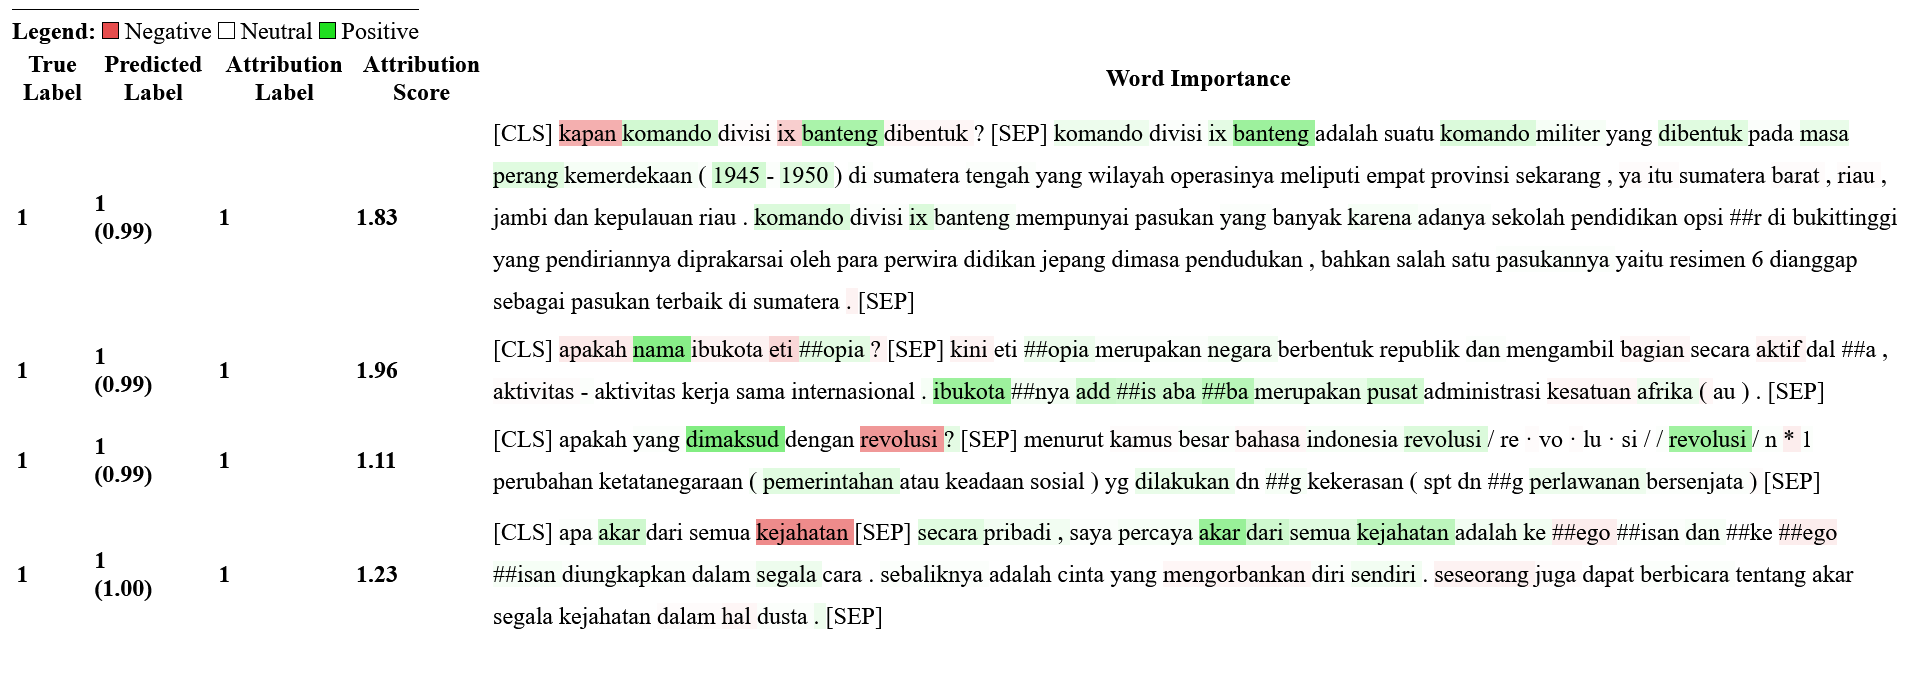
\includegraphics[width=1\textwidth]{assets/pics/IGBERTCAT.png}
    \caption{Interpretasi dari model $\text{BERT}_{CAT}$ dengan \f{integrated gradients}. Kata dengan warna hijau berarti kata tersebut berkontribusi positif terhadap hasil prediksi. Di lain sisi, kata yang berwarna merah berarti kata tersebut berkontribusi negatif terhadap hasil prediksi.}
    \label{fig:InterpretasiBERTCAT}
\end{figure}

Model berasitekturkan $\text{BERT}_{\text{DOT}}$ jauh lebih sulit untuk menginterpretasikannya. Hal yang dapat dilakukan adalah dengan menghitung nilai \f{importance} kata dengan menghitung hasil kali titik representasi vektor dari teks dengan representasi vektor masing-masing kata pada teks tersebut. Dengan hal ini, dapat nilai \f{importance} dari kata dapat diurutkan. \tab~\ref{tab:interpretasibertdot} menunjukkan kueri, teks dan 5 kata penting dari kueri dan teks tersebut.

\begin{table}
    \centering
    \caption{Interpretasi dari model $\text{BERT}_{\text{DOT}}$ dengan menghitung hasil kali titik antara vektor teks dengan vektor masing-masing kata pada teks tersebut. Hanya 5 kata dengan nilai \f{importance} tertinggi yang ditunjukkan.}
    \label{tab:interpretasibertdot}
    \begin{tabular}{|p{0.3\textwidth}|p{0.2\linewidth}| p{0.3\linewidth}| p{0.2\linewidth}|}
        \hline
        \textbf{Kueri} & \textbf{ 5 Kata Penting} & \textbf{Teks} & \textbf{ 5 Kata Penting} \\ \hline
        Kapan Petrus Lombardus lahir? & [lahir, petrus, kapan, lombardus, ?] & Petrus Lombardus mungkin dilahirkan di Novara; atau kemungkinan lainnya adalah di Lumellogno[7] (saat itu sebuah komune pedesaan, sekarang menjadi bagian dari Provinsi Novara, Piemonte), di barat laut Italia, dari suatu keluarga miskin.[8] Kelahirannya diperkirakan antara tahun 1095-1100. & [petrus, dilahirkan, kelahirannya, lombardus, keluarga] \\ 
        \hline
        Dimana Jamie Richard Vardy lahir? & [lahir, richard, jamie, ?, dimana] & Jamie Richard Vardy (lahir dengan nama Gill; 11 January 1987) adalah pemain sepak bola Inggris yang bermain di klub Premiere League Leicester City dan tim nasional Inggris. Ia bermain sebagai striker, namun juga bisa bermain di sayap & [gill, lahir, richard, tim, sepak] \\
        \hline
    \end{tabular}
\end{table}





\clearchapter
%---------------------------------------------------------------
\chapter{\kesimpulan}
\label{bab:6}
%---------------------------------------------------------------
Pada bab ini, penulis akan memaparkan kesimpulan penelitian dan saran untuk penelitian berikutnya.


%---------------------------------------------------------------
\section{Kesimpulan}
\label{sec:kesimpulan}
%---------------------------------------------------------------
Implementasi model \f{Bidirectional Encoder Representations from Transformers} (BERT) untuk pemeringkatan teks berbahasa Indonesia telah dilakukan pada \sect~\ref{bab:4}. Berikut ini adalah kesimpulan terkait pekerjaan yang dilakukan dalam penelitian ini:

\begin{enumerate}
	\item  Berdasarkan penjelasan pada \sect~\ref{bab:3} dan implementasi pada \sect~\ref{bab:4} telah ditunjukkan dua cara penggunaan BERT untuk pemeringakatan teks, yaitu BERT sebagai \f{soft classifier} dari nilai relevansi (kueri, teks) dan BERT sebagai pemetaan teks ke dalam ruang vektor dengan nilai skor relevansi dihitung dengan fungsi \f{similarity} seperti jarak kosinus dan \f{dot product}.
	\item \tab~\ref{tab:indobertcat-hasil} hingga \tab~\ref{tab:indobertkd-hasil} menunjukkan bahwa model BERT yang dilatih kembali (\f{fine tuning}) pada \f{dataset} Mmarco \f{train set} menghasilkan skor yang lebih baik dibandingkan dengan model \f{baseline} BM25 pada dua \f{dataset} uji Mmarco \f{dev set} dan MrTyDi \f{dev set}. Pada \f{dataset} Miracl \f{dev set}, hanya $\text{IndoBERT}_{\text{DOThardnegs}}$ yang menghasilkan skor yang lebih baik dibandingkan dengan model \f{baseline} BM25 pada metrik NDCG@10. dan $\text{IndoBERT}_{\text{CATs}}$ yang menghasilkan skor yang lebih baik pada metrik R@100.
\end{enumerate}

%---------------------------------------------------------------
\section{Saran}
\label{sec:saran}
%---------------------------------------------------------------
Berdasarkan hasil penelitian ini, berikut ini adalah saran untuk pengembangan penelitian berikutnya:
\begin{enumerate}
	\item Pelatihan model BERT dapat dilakukan dengan \f{dataset} yang lebih beragam. 
	\item Memperbanyak \f{dataset} uji untuk pemeringkatan teks, sehingga dapat dilakukan analisis yang lebih mendalam terhadap setiap model yang dihasilkan.
	\item Menambah jumlah model \f{baseline} untuk pemeringkatan teks. Beberapa model yang dapat ditambahkan adalah TF-IDF, Word2Vec, ELMo, dan arsitektur \f{non-transformer} seperti LSTM dan CNN.
\end{enumerate}

\clearchapter

%
% Daftar Pustaka
\CAPinToC % All entries in ToC will be CAPITALIZED from here on
\include{_internals/pustaka}
\clearchapter
\noCAPinToC % Revert to original \addcontentsline formatting

%
% Lampiran
%
\begin{appendix}
	\newcounter{pagetemp}
	\setcounter{pagetemp}{\thepage}
	\include{_internals/markLampiran}
	\clearchapter
	\setcounter{page}{\thepagetemp}
	\stepcounter{page}
	%-----------------------------------------------------------------------------%
\addappendix{Kode Simulasi}
\chapter*{Lampiran 1: Kode Simulasi}
\begin{enumerate}
    \item Repositori kode: \url{https://github.com/carlesoctav/beir-skripsi} 
    \item Repositori model dan data: \url{https://huggingface.co/carles-undergrad-thesis}
    \item Repositori data (\f{raw}): \url{https://drive.google.com/drive/folders/1l_fbqJSn2AR8f-g1QnANl5czm2aLO0rO}
\end{enumerate}

\lstinputlisting[language=Python, caption=Kode untuk mengevaluasi $\text{BERT}_{\text{DOT}}$, label=code:python]{assets/codes/beir-skripsi/experiments/hardnegs_bm25/eval_miracl_hardnegs.py}

\newpage

\lstinputlisting[language=Python, caption=Kode untuk mengevaluasi $\text{BERT}_{\text{CAT}}$, label=code:python]{assets/codes/beir-skripsi/experiments/bertcat_trained/eval_mrtydi_bertcat.py}

\newpage

\lstinputlisting[language=Python, caption=Kode untuk mengevaluasi BM25, label=code:python]{assets/codes/beir-skripsi/experiments/bm25/eval_miracl_bm25.py}

\newpage

\lstinputlisting[language=Python, caption=Kode untuk melatih  $\text{IndoBERT}_{\text{CAT}}$, label=code:python]{assets/codes/beir-skripsi/experiments/bertcat_trained/train.py}

\newpage

\lstinputlisting[language=Python, caption=Kode untuk melatih $\text{IndoBERT}_{\text{DOT}}$, label=code:python]{assets/codes/beir-skripsi/experiments/in_batch/train.py} 

\newpage

\lstinputlisting[language=Python, caption=Kode untuk melatih $\text{IndoBERT}_{\text{DOTKD}}$, label=code:python]{assets/codes/beir-skripsi/experiments/knowledge-distill-train/train.py}

\newpage

\lstinputlisting[language=Python, caption=Kode untuk melatih $\text{IndoBERT}_{\text{DOThardnegs}}$ dengan \f{hard negatives}, label=code:python]{assets/codes/beir-skripsi/experiments/hardnegs_bm25/train.py}



%-----------------------------------------------------------------------------%

%-----------------------------------------------------------------------------%
\addappendix{Tabel Metrik}
\chapter*{Lampiran 2: Tabel Metrik}
\label{appendix:metrik}

\begin{table}
    \centering
    \caption{Hasil evaluasi model pada Metrik \f{Reciprocal Rank} pada tiga \f{dataset} yang digunakan.}
    \label{tab:evalrr}
    \begin{tabular}{lccccc}
        \hline
        Model & RR@1 & RR@3 & RR@5 & RR@10 & RR@100 \\ 
        \hline
        \multicolumn{6}{c}{\textbf{mMARCO}} \\
        BM25 & 0.0662 & 0.0968 & 0.1061 & 0.1143 & 0.1226 \\
        BM25+$\text{IndoBERT}_{\text{CAT}}$  & 0.1053 & 0.1519 & 0.1660 & 0.1776 & 0.1865 \\ 
        $\text{IndoBERT}_{\text{DOT}}$ & 0.1033 & 0.1543 & 0.1696 & 0.1818 & 0.1924 \\
        $\text{IndoBERT}_{\text{DOThardnegs}} $ & 0.1483 & 0.2057 & 0.2208 & 0.2328 & 0.2430 \\
        $\text{IndoBERT}_{\text{DOTKD}}$ & 0.1476 & 0.2065 & 0.2222 & 0.2355 & 0.2461 \\
        \hline
        \multicolumn{6}{c}{\textbf{MrTyDI}} \\
        BM25 & 0.1858 & 0.2481 & 0.2659 & 0.2792 & 0.2898 \\
        BM25+$\text{IndoBERT}_{\text{CAT}}$  & 0.2459 & 0.3288 & 0.3479 & 0.3631 & 0.3720 \\
        $\text{IndoBERT}_{\text{DOT}}$ & 0.1918 & 0.2788 & 0.3068 & 0.3249 & 0.3349 \\
        $\text{IndoBERT}_{\text{DOThardnegs}} $ &  0.3764 & 0.4473 & 0.4608 & 0.4711 & 0.4779 \\
        $\text{IndoBERT}_{\text{DOTKD}}$ & 0.2955 & 0.3693 & 0.3849 & 0.3936 & 0.4013 \\
        \hline
        \multicolumn{6}{c}{\textbf{Miracl}} \\
        BM25 & 0.3510 & 0.4385 & 0.4596 & 0.4723 & 0.4815 \\
        BM25+$\text{IndoBERT}_{\text{CAT}}$  & 0.2938 & 0.3951 & 0.4210 & 0.4373 & 0.4467 \\
        $\text{IndoBERT}_{\text{DOT}}$ & 0.2385 & 0.3450 & 0.3658 & 0.3808 & 0.3920 \\
        $\text{IndoBERT}_{\text{DOThardnegs}} $ & 0.4146 & 0.4901 & 0.5070 & 0.5170 & 0.5238 \\
        $\text{IndoBERT}_{\text{DOTKD}}$ & 0.3719 & 0.4509 & 0.4697 & 0.4788 & 0.4855 \\
        \hline
        
        \end{tabular}
        
\end{table}


\newpage

\begin{table}
    \centering
    \caption{Hasil evaluasi model pada Metrik \f{Recall} pada tiga \f{dataset} yang digunakan.}
    \label{tab:evalrecall}
    \begin{tabular}{lccccc}
        \hline
        Model & R@1 & R@3 & R@5 & R@10 & R@100 \\ 
        \hline
        \multicolumn{6}{c}{\textbf{mMARCO}} \\
        BM25 & 0.0641 & 0.1334 & 0.1735 & 0.2350 & 0.4475 \\
        BM25+$\text{IndoBERT}_{\text{CAT}}$  & 0.1026 & 0.2074 & 0.2691 & 0.3551 & 0.5685 \\ 
        $\text{IndoBERT}_{\text{DOT}}$ & 0.1010 & 0.2168 & 0.2824 & 0.3724 & 0.6506 \\
        $\text{IndoBERT}_{\text{DOThardnegs}} $ & 0.1444 & 0.2738 & 0.3383 & 0.4273 & 0.6807 \\
        $\text{IndoBERT}_{\text{DOTKD}}$ & 0.1436 & 0.2768 & 0.3446 & 0.4427 & 0.7052 \\
        \hline
        \multicolumn{6}{c}{\textbf{MrTyDI}} \\
        BM25 & 0.1705 & 0.3040 & 0.3828 & 0.4755 & 0.7230 \\
        BM25+$\text{IndoBERT}_{\text{CAT}}$  & 0.2459& 0.4363 & 0.5196 & 0.6332 & 0.8301 \\
        $\text{IndoBERT}_{\text{DOT}}$ & 0.1707 & 0.3639 & 0.4811 & 0.6118 & 0.8520 \\
        $\text{IndoBERT}_{\text{DOThardnegs}} $ & 0.3428 & 0.5018 & 0.5657 & 0.6496 & 0.8247 \\
        $\text{IndoBERT}_{\text{DOTKD}}$ & 0.2680 & 0.4323 & 0.5022 & 0.5700 & 0.7513 \\
        \hline
        \multicolumn{6}{c}{\textbf{Miracl}} \\
        BM25 & 0.1652 & 0.2899 & 0.3636 & 0.4734 & 0.8116 \\
        BM25+$\text{IndoBERT}_{\text{CAT}}$  & 0.1302 & 0.2701 & 0.3564 & 0.4802 & 0.8535 \\
        $\text{IndoBERT}_{\text{DOT}}$ & 0.1089 & 0.2475 & 0.3145 & 0.4146 & 0.7415 \\
        $\text{IndoBERT}_{\text{DOThardnegs}} $ & 0.1787 & 0.3043 & 0.3678 & 0.4552 & 0.7266 \\
        $\text{IndoBERT}_{\text{DOTKD}}$ & 0.1635 & 0.2883 & 0.3552 & 0.4322 & 0.7025 \\
        \hline
        
        \end{tabular}
        
\end{table}


\newpage


\begin{table}
    \centering
    \caption{Hasil evaluasi model pada Metrik \f{ndcg} pada tiga \f{dataset} yang digunakan.}
    \label{tab:evalndcg}
    \begin{tabular}{lccccc}
        \hline
        Model & NDCG@1 & NDCG@3 & NDCG@5 & NDCG@10 & NDCG@100 \\
        \hline
        \multicolumn{6}{c}{\textbf{mMARCO}} \\
        BM25 & 0.0660 & 0.1048 & 0.1215 & 0.1415 & 0.1857 \\
        BM25+$\text{IndoBERT}_{\text{CAT}}$  & 0.1055 & 0.1644 & 0.1900 & 0.2182 & 0.2638 \\
        $\text{IndoBERT}_{\text{DOT}}$ & 0.1034 & 0.1687 & 0.1960 & 0.2254 & 0.2830 \\
        $\text{IndoBERT}_{\text{DOThardnegs}} $ & 0.1483 & 0.2212 & 0.2480 & 0.2771 & 0.3305 \\
        $\text{IndoBERT}_{\text{DOTKD}}$ & 0.1476 & 0.2223 & 0.2505 & 0.2826 & 0.3379 \\
        \hline
        \multicolumn{6}{c}{\textbf{MrTyDI}} \\
        BM25 & 0.1846 & 0.2527 & 0.2860 & 0.3170 & 0.3727 \\
        BM25+$\text{IndoBERT}_{\text{CAT}}$  & 0.2459 & 0.3563 & 0.3905 & 0.4274 & 0.4700 \\
        $\text{IndoBERT}_{\text{DOT}}$  & 0.1918 & 0.2916 & 0.3413 & 0.3858 & 0.4391 \\
        $\text{IndoBERT}_{\text{DOThardnegs}} $ & 0.3764 & 0.4467 & 0.4743 & 0.5026 & 0.5404 \\
        $\text{IndoBERT}_{\text{DOTKD}}$ & 0.2955 & 0.3734 & 0.4030 & 0.4255 & 0.4657 \\
        \hline
        \multicolumn{6}{c}{\textbf{Miracl}} \\
        BM25 & 0.3510 & 0.3373 & 0.3531 & 0.3915 & 0.4935 \\
        BM25+$\text{IndoBERT}_{\text{CAT}}$  & 0.2938 & 0.2984 & 0.3226 & 0.3673 & 0.4802 \\
        $\text{IndoBERT}_{\text{DOT}}$ & 0.2385 & 0.2655 & 0.2834 & 0.3196 & 0.4188 \\
        $\text{IndoBERT}_{\text{DOThardnegs}} $ & 0.4146 & 0.3688 & 0.3700 & 0.3977 & 0.4776 \\
        $\text{IndoBERT}_{\text{DOTKD}}$ & 0.3719 & 0.3419 & 0.3503 & 0.3741 & 0.4542 \\
        \hline
        \end{tabular}
        
\end{table}

\newpage

\begin{table}
    \centering
    \caption{Hasil evaluasi model pada Metrik \f{Precision} pada tiga \f{dataset} yang digunakan.}
    \label{tab:evalprecision}
    \begin{tabular}{lccccc}
        \hline
        Model & P@1 & P@3 & P@5 & P@10 & P@100 \\
        \hline
        \multicolumn{6}{c}{\textbf{mMARCO}} \\
        BM25 & 0.0660 & 0.0459 & 0.0360 & 0.0245 & 0.0047 \\
        BM25+$\text{IndoBERT}_{\text{CAT}}$  & 0.1055 & 0.0717 & 0.0560 & 0.0371 & 0.0060 \\
        $\text{IndoBERT}_{\text{DOT}}$ & 0.01034 & 0.0744 & 0.0583 & 0.0387 & 0.0068 \\
        $\text{IndoBERT}_{\text{DOThardnegs}} $ & 0.1483 & 0.0942 & 0.0701 & 0.0444 & 0.0072 \\
        $\text{IndoBERT}_{\text{DOTKD}}$ &  0.1476 & 0.0956 & 0.0716 & 0.0461 & 0.0074 \\
        \hline
        \multicolumn{6}{c}{\textbf{MrTyDI}} \\
        BM25 & 0.1846 & 0.1122 & 0.0849 & 0.0532 & 0.0083 \\
        BM25+$\text{IndoBERT}_{\text{CAT}}$  & 0.2459 & 0.1454 & 0.1039 & 0.0633 & 0.0083 \\
        $\text{IndoBERT}_{\text{DOT}}$ & 0.1918 & 0.1367 & 0.1086 & 0.0698 & 0.0098 \\
        $\text{IndoBERT}_{\text{DOThardnegs}} $ & 0.3764 & 0.1870 & 0.1279 & 0.0742 & 0.0095 \\
        $\text{IndoBERT}_{\text{DOTKD}}$ & 0.2955 & 0.1616 & 0.1129 & 0.0640 & 0.0086 \\
        \hline
        \multicolumn{6}{c}{\textbf{Miracl}} \\
        BM25 & 0.3510 & 0.2427 & 0.1975 & 0.1352 & 0.0256 \\
        BM25+$\text{IndoBERT}_{\text{CAT}}$  & 0.2938 & 0.2212 & 0.1829 & 0.1288 & 0.0267 \\
        $\text{IndoBERT}_{\text{DOT}}$ & 0.2385 & 0.2004 & 0.1631 & 0.1144 & 0.0232 \\
        $\text{IndoBERT}_{\text{DOThardnegs}} $ & 0.4146 & 0.2611 & 0.1963 & 0.1290 & 0.0225 \\
        $\text{IndoBERT}_{\text{DOTKD}}$ & 0.3719 & 0.2465 & 0.1933 & 0.1247 & 0.0221 \\
        \hline
        
        \end{tabular}
        
\end{table}

\newpage

\begin{table}
    \centering
    \caption{Hasil evaluasi model pada Metrik \f{Mean Average Precision} pada tiga \f{dataset} yang digunakan.}
    \label{tab:evalmap}
    \begin{tabular}{lccccc}
        \hline
        Model & MAP@1 & MAP@3 & MAP@5 & MAP@10 & MAP@100 \\
        \hline
        \multicolumn{6}{c}{\textbf{mMARCO}} \\
        BM25 & 0.0641 & 0.0940 & 0.1033 & 0.1116 & 0.1199 \\
        BM25+$\text{IndoBERT}_{\text{CAT}}$  & 0.1026 & 0.1482 & 0.1625 & 0.1742 & 0.1833 \\
        $\text{IndoBERT}_{\text{DOT}}$ & 0.010 & 0.1510 & 0.1661 & 0.1783 & 0.1892 \\
        $\text{IndoBERT}_{\text{DOThardnegs}} $ & 0.1444 & 0.2016 & 0.2165 & 0.2285 & 0.2390 \\
        $\text{IndoBERT}_{\text{DOTKD}}$ & 0.1436 & 0.2019 & 0.2176 & 0.2310 & 0.2418 \\
        \hline
        \multicolumn{6}{c}{\textbf{MrTyDI}} \\
        BM25 & 0.1705 & 0.2284 & 0.2475 & 0.2605 & 0.2731 \\
        BM25+$\text{IndoBERT}_{\text{CAT}}$  & 0.2459 & 0.3287 & 0.3476 & 0.3630 & 0.3719 \\
        $\text{IndoBERT}_{\text{DOT}}$ & 0.1707 & 0.2603 & 0.2883 & 0.3077 & 0.3194 \\
        $\text{IndoBERT}_{\text{DOThardnegs}} $ & 0.3428 & 0.4181 & 0.4349 & 0.4475 & 0.4553 \\
        $\text{IndoBERT}_{\text{DOTKD}}$ & 0.2680 & 0.3450 & 0.3622 & 0.3719 & 0.3806 \\
        \hline
        \multicolumn{6}{c}{\textbf{Miracl}} \\
        BM25 & 0.1652 & 0.2395 & 0.2685 & 0.2987 & 0.3323 \\
        BM25+$\text{IndoBERT}_{\text{CAT}}$  & 0.1302 & 0.2059 & 0.2360 & 0.2657 & 0.3010 \\
        $\text{IndoBERT}_{\text{DOT}}$ & 0.1089 & 0.1827 & 0.2062 & 0.2302 & 0.2600 \\
        $\text{IndoBERT}_{\text{DOThardnegs}} $ & 0.1787 & 0.2573 & 0.2820 & 0.3054 & 0.3297 \\
        $\text{IndoBERT}_{\text{DOTKD}}$ & 0.1635 & 0.2388 & 0.2655 & 0.2864 & 0.3114 \\
        \hline        
        \end{tabular}        
\end{table}

\end{appendix}

\end{document}
